\input{"preamble.tex"}

\addbibresource{UGA\_Topology\_Qual\_Solutions.bib}

\let\Begin\begin
\let\End\end
\newcommand\wrapenv[1]{#1}

\makeatletter
\def\ScaleWidthIfNeeded{%
 \ifdim\Gin@nat@width>\linewidth
    \linewidth
  \else
    \Gin@nat@width
  \fi
}
\def\ScaleHeightIfNeeded{%
  \ifdim\Gin@nat@height>0.9\textheight
    0.9\textheight
  \else
    \Gin@nat@width
  \fi
}
\makeatother

\setkeys{Gin}{width=\ScaleWidthIfNeeded,height=\ScaleHeightIfNeeded,keepaspectratio}%

\title{
\textbf{
    Topology Qualifying Exam Solutions
  }
  }







\begin{document}

\date{}
\author{D. Zack Garza}
\maketitle


\newpage

% Note: addsec only in KomaScript
\addsec{Table of Contents}
\tableofcontents
\newpage

\hypertarget{preface}{%
\section{Preface}\label{preface}}

A great deal of credit for this document goes to Mike Usher, who created
an initial PDF of past UGA qual questions organized by topic. Here is a
list of problems that Mike recommended reviewing during our problem
sessions in Spring 2020:

\begin{itemize}
\tightlist
\item
  Section 1, Point-Set: 8, 10, 11, 14, 16, 19, 22, 23, 27 (Bolzano
  Weierstrass), 30 (Standard, see counterexamples), 31, 32, 38, 42, 44
\item
  Section 2, Fundamental Group: 1
\item
  Section 3, Covering Spaces: 1b and c, 2, 3, 6, 7, 8, 10 (not really
  about surfaces per se), 11, 12, 13, 14, 16
\item
  Section 4, Homology/Degree Theory: 2, 4, 5, 8, 13, 19, 21, 22
\item
  Section 5, Cell Complexes/Attaching: 1, 5, 10, 16
\item
  Section 6, Surfaces: 3, 6, 7, 11, 14
\item
  Section 7, Fixed Points: 4, 6, 12, 13, 14
\item
  Section 8, Misc Algebraic Topology: 1, 3, 6, 8
\end{itemize}

\begin{warnings}

Usually 30\% of the problems on any given qual are related to
point-set/general Topology. Note that this material is not covered in
the course!

\end{warnings}

\hypertarget{general-topology}{%
\section{General Topology}\label{general-topology}}

\hypertarget{topologies-subspaces-closures-and-maps}{%
\subsection{Topologies, Subspaces, Closures, and
Maps}\label{topologies-subspaces-closures-and-maps}}

\hypertarget{fall-11-done}{%
\subsubsection{\texorpdfstring{Fall '11
\(\done\)}{Fall '11 \textbackslash done}}\label{fall-11-done}}

\begin{problem}[Fall 2011]

Let \(X\) be a topological space, and \(B \subset A \subset X\). Equip
\(A\) with the subspace topology, and write
\({ \operatorname{cl}} _X (B)\) or \({ \operatorname{cl}} _A (B)\) for
the closure of \(B\) as a subset of, respectively, \(X\) or \(A\).

Determine, with proof, the general relationship between
\({ \operatorname{cl}} _X (B) \cap A\) and
\({ \operatorname{cl}} _A (B)\)

\begin{quote}
I.e., are they always equal? Is one always contained in the other but
not conversely? Neither?
\end{quote}

\end{problem}

\begin{concept}

\envlist

\begin{itemize}
\tightlist
\item
  Definition of closure: for \(A\subseteq X\),
  \({ \operatorname{cl}} _X(A)\) is the intersection of all
  \(B\supseteq A\) which are closed in \(X\).
\item
  Definition of ``relative'' closure: for \(A\subseteq Y \subseteq X\),
  \({ \operatorname{Cl}} _Y(A)\) is the intersection of all \(B\) such
  that \(Y\supseteq B \supseteq A\) which are closed in \(Y\).
\item
  Closed sets in a subspace: \(B' \subseteq Y\subseteq X\) is closed in
  \(Y\) if \(B' = B\cap Y\) for some \(B'\) closed in \(X\).
\end{itemize}

\end{concept}

\begin{strategy}

What's the picture? Just need to remember what the closure with respect
to a subspace looks like:

\begin{figure}
\centering
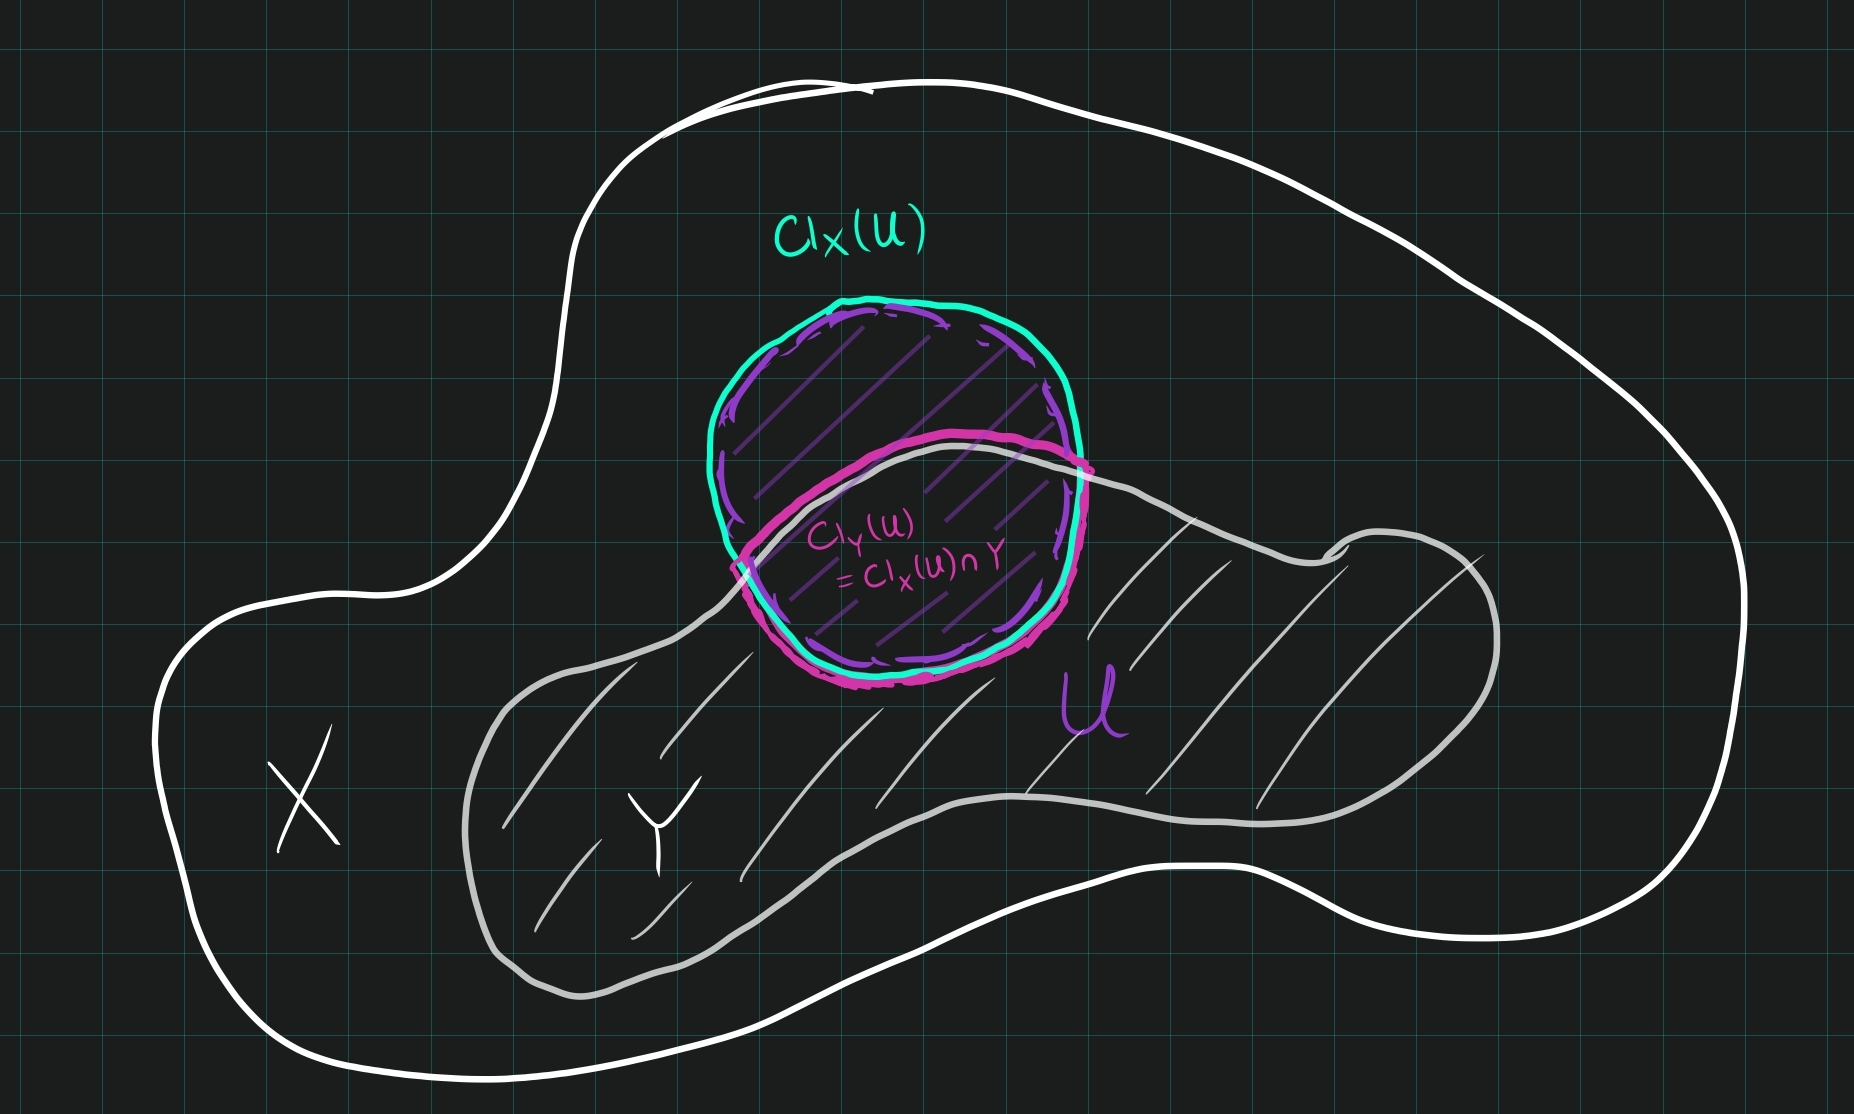
\includegraphics{figures/image_2021-05-20-23-58-56.png}
\caption{image\_2021-05-20-23-58-56}
\end{figure}

\end{strategy}

\begin{solution}

\envlist

\begin{itemize}
\tightlist
\item
  Claim:
  \({ \operatorname{Cl}} _X(A) \cap Y = { \operatorname{Cl}} _Y(A)\).
\item
  Write \({ \operatorname{Cl}} _Y(A)\) as the intersection of \(B'\)
  where \(Y\supseteq B' \supseteq A\) with \(B'\) closed in \(Y\).
\item
  Every such \(B'\) is of the form \(B' = B \cap Y\) for some \(B\)
  closed in \(X\).
\item
  Just identify the two sides directly by reindexing the intersection:
  \begin{align*}
  { \operatorname{Cl}} _Y(A) 
  &\coloneqq\displaystyle\bigcap_{\substack{ Y\supseteq B' \supseteq A \\ B' \text{ closed in } Y}} B' \\
  &= \displaystyle\bigcap_{\substack{ X \supseteq B \cap Y \supseteq A \\ B \text{ closed in } X}} \qty{ B \cap Y } \\
  &= \qty{ \displaystyle\bigcap_{\substack{ X \supseteq B \cap Y \supseteq A \\ B \text{ closed in } X}} B} \cap Y \\ \\
  &\coloneqq{ \operatorname{Cl}} _X(A) \cap Y
  .\end{align*}
\end{itemize}

\end{solution}

\hypertarget{fall-05-done}{%
\subsubsection{\texorpdfstring{6 (Fall '05)
\(\done\)}{6 (Fall '05) \textbackslash done}}\label{fall-05-done}}

\begin{problem}[Fall 2005]

Prove that the unit interval \(I\) is compact. Be sure to explicitly
state any properties of \({\mathbb{R}}\) that you use.

\end{problem}

\begin{concept}

\envlist

\begin{itemize}
\tightlist
\item
  Cantor's intersection theorem: for a topological space, any nested
  sequence of compact nonempty sets has nonempty intersection.
\item
  Bases for standard topology on \({\mathbb{R}}\).
\item
  Definition of compactness
\end{itemize}

\end{concept}

\begin{strategy}

What's the picture? Similar to covering
\(\left\{{1\over n}\right\}\cup\left\{{0}\right\}\): cover \(x=0\) with
one set, which nets all but finitely many points.

\begin{figure}
\centering
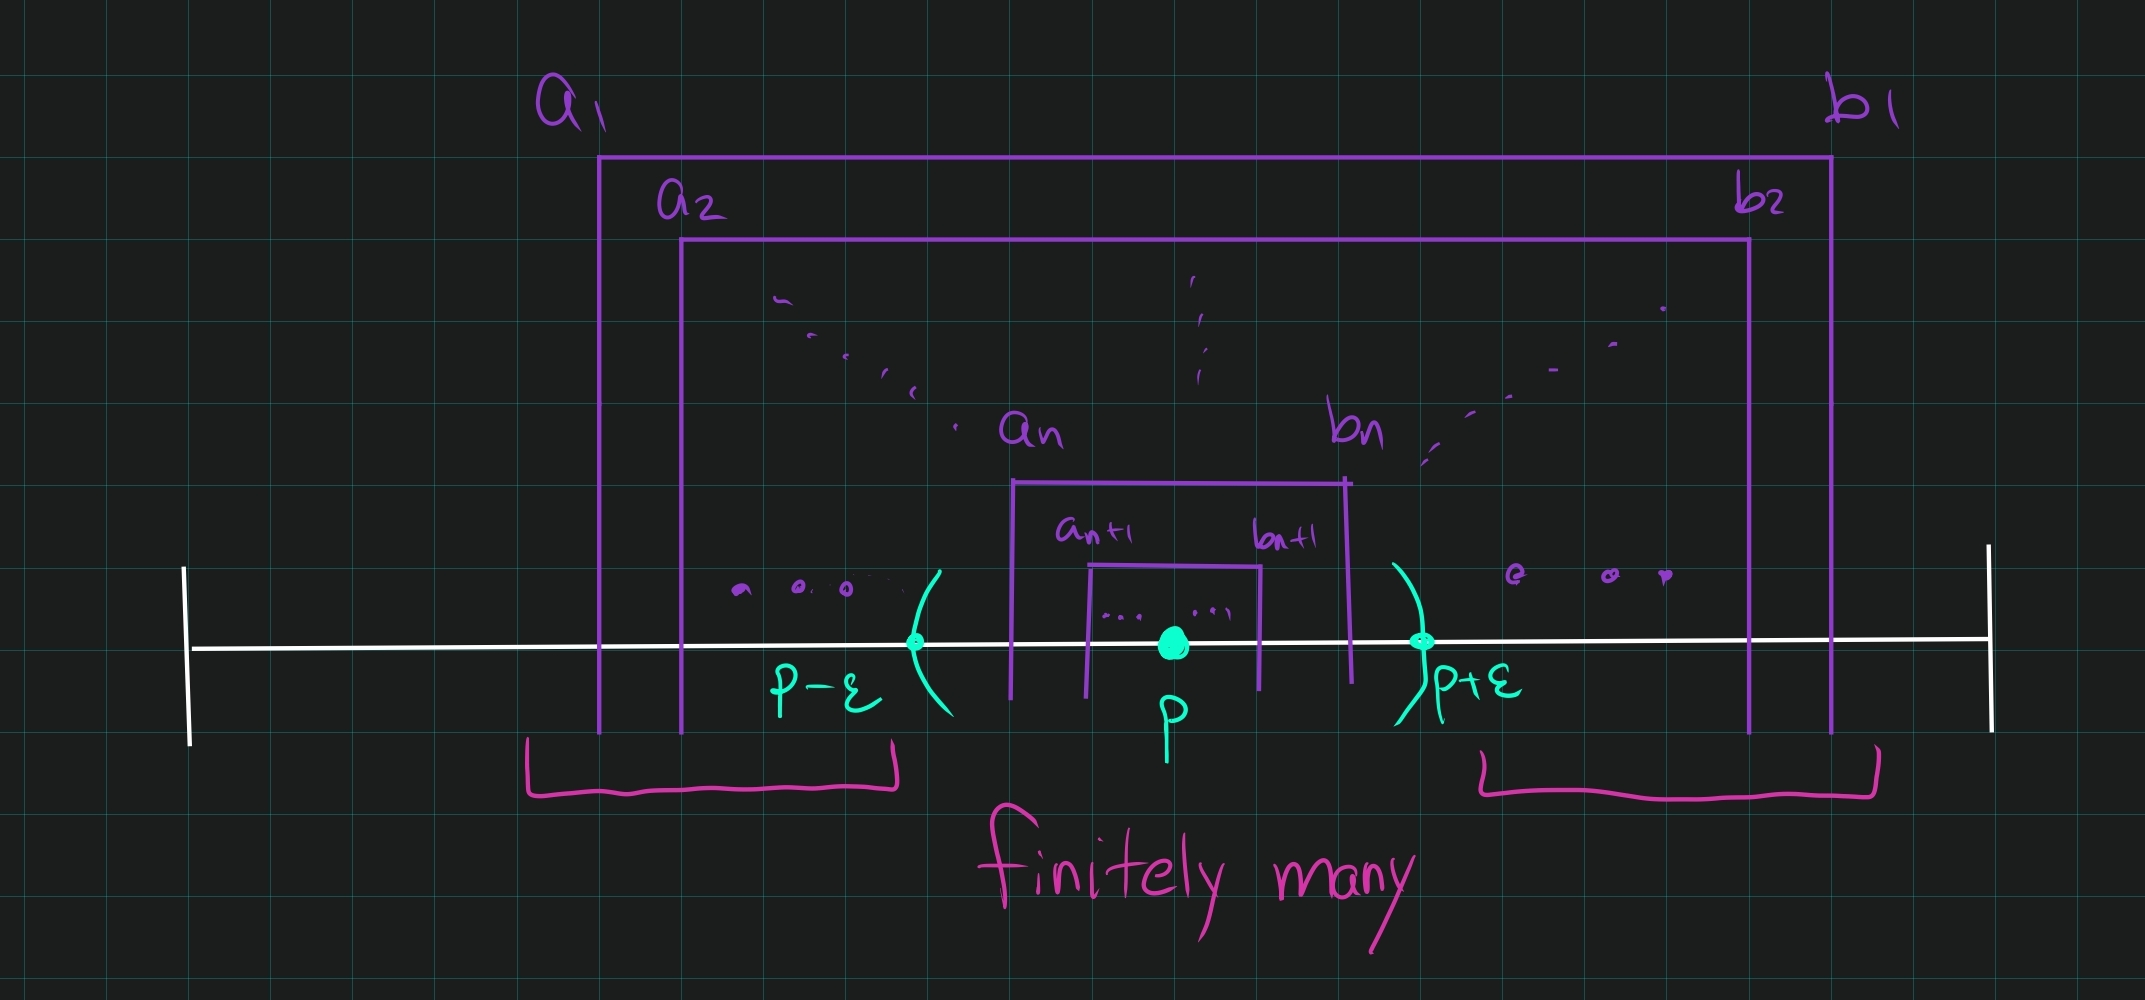
\includegraphics{figures/image_2021-05-20-22-46-54.png}
\caption{image\_2021-05-20-22-46-54}
\end{figure}

Proceed by contradiction. Binary search down into nested intervals, none
of which have finite covers. Get a single point, a single set which
eventually contains all small enough nested intervals. Only need
finitely many more opens to cover the rest.

\end{strategy}

\begin{solution}

\envlist

\begin{itemize}
\tightlist
\item
  Toward a contradiction, let
  \(\left\{{U_\alpha}\right\} \rightrightarrows[0, 1]\) be an open cover
  with no finite subcover.
\item
  Then either \([0, {1\over 2}]\) or \([{1\over 2}, 1]\) has no finite
  subcover; WLOG assume it is \([0, {1\over 2}]\).
\item
  Then either \([0, {1\over 4}]\) or \([{1\over 4}, {1\over 2}]\) has no
  finite subcover
\item
  Inductively defining \([a_n, b_n]\) this way yields a sequence of
  compact nested intervals (each with no finite subcover) so Cantor's
  Nested Interval theorem applies.
\item
  Since \({\mathbb{R}}\) is a complete metric space and the diameters
  \({\operatorname{diam}}([a_n, b_n]) \leq {1 \over 2^n} \to 0\), the
  intersection contains exactly one point.
\item
  Since \(p\in [0, 1]\) and the \(U_\alpha\) form an open cover,
  \(p\in U_\alpha\) for some \(\alpha\).
\item
  Since a basis for \(\tau({\mathbb{R}})\) is given by open intervals,
  we can find an \(\varepsilon>0\) such that
  \((p-\varepsilon, p+\varepsilon) \subseteq U_\alpha\)
\item
  Then if \({1\over 2^N} < \varepsilon\), for \(n\geq N\) we have
  \begin{align*}[a_n, b_n] \subseteq (p-\varepsilon, p+\varepsilon) \subseteq U_\alpha.\end{align*}
\item
  But then \(U_\alpha \rightrightarrows[a_n, b_n]\), yielding a finite
  subcover of \([a_n, b_n]\), a contradiction.
\end{itemize}

\end{solution}

\hypertarget{fall-06.-work}{%
\subsubsection{\texorpdfstring{7 (Fall '06).
\(\work\)}{7 (Fall '06). \textbackslash work}}\label{fall-06.-work}}

\begin{problem}[Fall 2006, 7]

A topological space is \textbf{sequentially compact} if every infinite
sequence in \(X\) has a convergent subsequence.

Prove that every compact metric space is sequentially compact.

\end{problem}

\hypertarget{fall-10.-done}{%
\subsubsection{\texorpdfstring{8 (Fall '10).
\(\done\)}{8 (Fall '10). \textbackslash done}}\label{fall-10.-done}}

\begin{problem}[Fall 2010, 8]

Show that for any two topological spaces \(X\) and \(Y\) ,
\(X \times Y\) is compact if and only if both \(X\) and \(Y\) are
compact.

\end{problem}

\begin{concept}

\envlist

\begin{itemize}
\tightlist
\item
  Proof of the tube lemma:
\item
  Continuous image of compact is compact.
\end{itemize}

\end{concept}

\begin{strategy}

What's the picture?

\begin{figure}
\centering
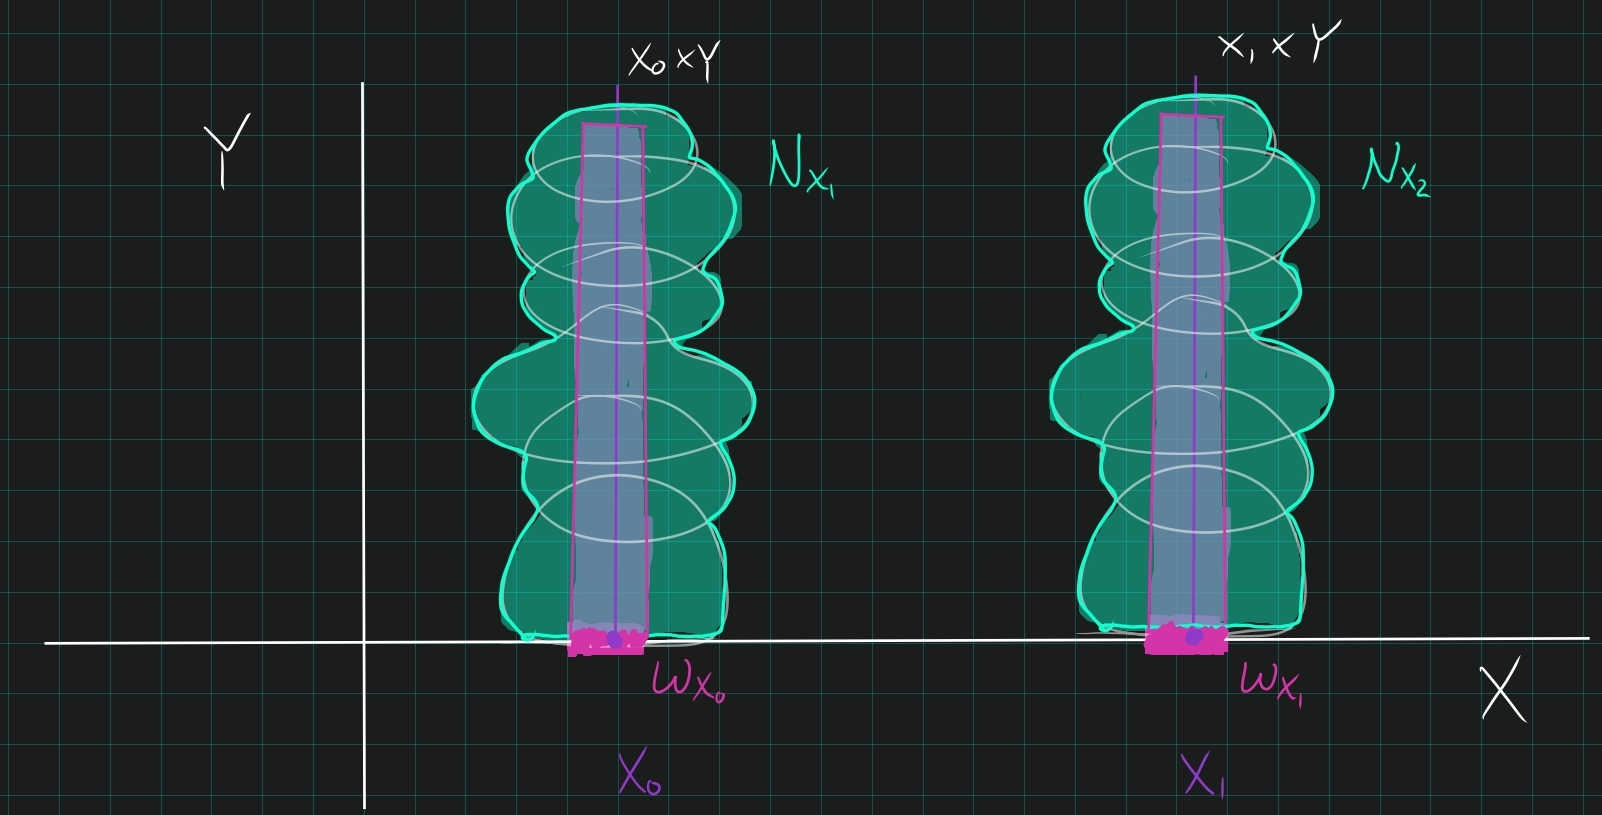
\includegraphics{figures/image_2021-05-21-01-16-52.png}
\caption{image\_2021-05-21-01-16-52}
\end{figure}

Take an open cover of the product, use that vertical fibers are compact
to get a finite cover for each fiber. Use tube lemma to get opens in the
base space, run over all \(x\) so the tube bases cover \(X\). Use that
\(X\) is compact to get a finite subcover.

\end{strategy}

\begin{solution}

\envlist

\begin{proof}[Using the tube lemma without proof]

\(\impliedby\):

\begin{itemize}
\tightlist
\item
  By the universal property, the product \(X\times Y\) is equipped with
  continuous projections \(\pi_X: X\times Y\to X\) and
  \(\pi_Y: X\times Y\to X\).
\item
  The continuous image of a compact space is compact, and the images are
  all of \(X\) and \(Y\) respectively:
  \begin{align*}
  \pi_1(X\times Y) &= X \\
  \pi_2(X\times Y) &= Y
  .\end{align*}
\end{itemize}

\(\implies\):

\begin{itemize}
\item
  Let \(\left\{{U_j}\right\} \rightrightarrows X\times Y\) be an open
  cover.
\item
  \textbf{Cover a fiber}: fix \(x\in X\), the slice \(x \times Y\) is
  homeomorphic to \(Y\) and thus compact
\item
  Cover it by finitely many elements
  \(\left\{{U_j}\right\}_{j\leq m} \rightrightarrows{x} \times Y\).

  \begin{quote}
  Really, cover \(Y\), and then cross with \(x\) to cover
  \(x \times Y\).
  \end{quote}

  \begin{itemize}
  \tightlist
  \item
    Set
    \begin{align*}
    N_x \coloneqq\displaystyle\bigcup_{j\leq m} U_j \supseteq x \times Y
    .\end{align*}
  \item
    Apply the tube lemma to \(N_x\):

    \begin{itemize}
    \tightlist
    \item
      Produce a neighborhood \(W_x\) of \(x\) in \(X\) where
      \(W_x \subset N_x\)
    \item
      This yields a finite cover:
      \begin{align*}
      \left\{{U_j}\right\}_{j\leq m}\rightrightarrows N_x \times Y \supset W_x \times Y \implies \left\{{U_j}\right\}_{j\leq m} \rightrightarrows W_x\times Y
      .\end{align*}
    \end{itemize}
  \end{itemize}
\item
  \textbf{Cover the base}: let \(x\in X\) vary: for each \(x\in X\),
  produce \(W_x \times Y\) as above, then
  \(\left\{{W_x}\right\}_{x\in X} \rightrightarrows X\) where each tube
  \(W_x \times Y\) is covered by \emph{finitely} many \(U_j\).
\item
  Use that \(X\) is compact to produce a finite subcover
  \(\left\{{W_k}\right\}_{k \leq M} \rightrightarrows X\).
\item
  Then
  \(\left\{{W_k\times Y}\right\}_{k\leq M} \rightrightarrows X\times Y\),
  this is a finite set since each fiber was covered by finitely many
  opens

  \begin{itemize}
  \tightlist
  \item
    Finitely many \(k\)
  \item
    For each \(k\), the tube \(W_k \times Y\) is covered by finitely by
    \(U_j\)
  \item
    And finite \(\times\) finite = finite.
  \end{itemize}
\end{itemize}

\end{proof}

\end{solution}

\hypertarget{spring-06.-work}{%
\subsubsection{\texorpdfstring{12 (Spring '06).
\(\work\)}{12 (Spring '06). \textbackslash work}}\label{spring-06.-work}}

\begin{problem}[Spring 2006, 12]

Write \(Y\) for the interval \([0, \infty)\), equipped with the usual
topology.

Find, with proof, all subspaces \(Z\) of \(Y\) which are retracts of
\(Y\).

\end{problem}

\todo[inline]{Not finished. Add concepts}

\begin{solution}

\envlist

\begin{itemize}
\tightlist
\item
  Using the fact that \([0, \infty) \subset {\mathbb{R}}\) is Hausdorff,
  any retract must be closed, so any closed interval
  \([\varepsilon, N]\) for \(0\leq \varepsilon\leq N \leq \infty\).

  \begin{itemize}
  \tightlist
  \item
    Note that \(\varepsilon= N\) yields all one point sets
    \(\left\{{x_0}\right\}\) for \(x_0 \geq 0\).
  \end{itemize}
\item
  No finite discrete sets occur, since the retract of a connected set is
  connected.
\end{itemize}

\end{solution}

\hypertarget{fall-06.-work-1}{%
\subsubsection{\texorpdfstring{13 (Fall '06).
\(\work\)}{13 (Fall '06). \textbackslash work}}\label{fall-06.-work-1}}

\begin{problem}[Fall 2006, 13]

\envlist

\begin{enumerate}
\def\labelenumi{\alph{enumi}.}
\item
  Prove that if the space \(X\) is connected and locally path connected
  then \(X\) is path connected.
\item
  Is the converse true? Prove or give a counterexample.
\end{enumerate}

\end{problem}

\hypertarget{fall-07-work}{%
\subsubsection{\texorpdfstring{14 (Fall '07)
\(\work\)}{14 (Fall '07) \textbackslash work}}\label{fall-07-work}}

\begin{problem}[?]

Let \(\left\{{X_\alpha \mathrel{\Big|}\alpha \in A}\right\}\) be a
family of connected subspaces of a space \(X\) such that there is a
point \(p \in X\) which is in each of the \(X_\alpha\).

Show that the union of the \(X_\alpha\) is connected.

\end{problem}

\todo[inline]{Proof 2 not complete?}

\begin{solution}

\envlist

\begin{proof}[Variant 1]

\begin{itemize}
\tightlist
\item
  Take two connected sets \(X, Y\); then there exists \(p\in X\cap Y\).
\item
  Toward a contradiction: write \(X\cup Y = A {\textstyle\coprod}B\)
  with both \(A, B \subset A{\textstyle\coprod}B\) open.
\item
  Since \(p\in X \cup Y = A{\textstyle\coprod}B\), WLOG \(p\in A\). We
  will show \(B\) must be empty.
\item
  Claim: \(A\cap X\) is clopen in \(X\).

  \begin{itemize}
  \tightlist
  \item
    \(A\cap X\) is open in \(X\): ?
  \item
    \(A\cap X\) is closed in \(X\): ?
  \end{itemize}
\item
  The only clopen sets of a connected set are empty or the entire thing,
  and since \(p\in A\), we must have \(A\cap X = X\).
\item
  By the same argument, \(A\cap Y = Y\).
\item
  So \(A\cap\qty{X\cup Y} = \qty{A\cap X} \cup\qty{A\cap Y} = X\cup Y\)
\item
  Since \(A\subset X\cup Y\), \(A\cap\qty{X\cup Y} = A\)
\item
  Thus \(A = X\cup Y\), forcing \(B = \emptyset\).
\end{itemize}

\end{proof}

\begin{proof}[Variant 2]

Let \(X \coloneqq\cup_\alpha X_\alpha\), and let \(p\in \cap X_\alpha\).
Suppose toward a contradiction that \(X = A {\textstyle\coprod}B\) with
\(A,B\) nonempty, disjoint, and relatively open as subspaces of \(X\).
Wlog, suppose \(p\in A\), so let \(q\in B\) be arbitrary.

Then \(q\in X_\alpha\) for some \(\alpha\), so \(q\in B \cap X_\alpha\).
We also have \(p\in A \cap X_\alpha\).

But then these two sets disconnect \(X_\alpha\), which was assumed to be
connected -- a contradiction.

\end{proof}

\end{solution}

\hypertarget{fall-04.-work}{%
\subsubsection{\texorpdfstring{5 (Fall '04).
\(\work\)}{5 (Fall '04). \textbackslash work}}\label{fall-04.-work}}

\begin{problem}[?]

Let \(X\) be a topological space.

\begin{enumerate}
\def\labelenumi{\alph{enumi}.}
\item
  Prove that \(X\) is connected if and only if there is no continuous
  nonconstant map to the discrete two-point space
  \(\left\{{0, 1}\right\}\).
\item
  Suppose in addition that \(X\) is compact and \(Y\) is a connected
  Hausdorff space. Suppose further that there is a continuous map
  \(f : X \to Y\) such that every preimage \(f^{-1}(y)\) for
  \(y \in Y\), is a connected subset of \(X\).
\end{enumerate}

Show that \(X\) is connected.

\begin{enumerate}
\def\labelenumi{\alph{enumi}.}
\setcounter{enumi}{2}
\tightlist
\item
  Give an example showing that the conclusion of (b) may be false if
  \(X\) is not compact.
\end{enumerate}

\end{problem}

\hypertarget{spring-10-done}{%
\subsubsection{\texorpdfstring{? (Spring '10)
\(\done\)}{? (Spring '10) \textbackslash done}}\label{spring-10-done}}

\begin{problem}[?]

If \(X\) is a topological space and \(S \subset X\), define in terms of
open subsets of \(X\) what it means for \(S\) \textbf{not} to be
connected.

Show that if \(S\) is not connected there are nonempty subsets
\(A, B \subset X\) such that
\begin{align*}
A \cup B = S {\quad \operatorname{and} \quad} A \cap \mkern 1.5mu\overline{\mkern-1.5muB\mkern-1.5mu}\mkern 1.5mu = \mkern 1.5mu\overline{\mkern-1.5muA\mkern-1.5mu}\mkern 1.5mu \cap B = \emptyset
\end{align*}

\begin{quote}
Here \(\mkern 1.5mu\overline{\mkern-1.5muA\mkern-1.5mu}\mkern 1.5mu\)
and \(\mkern 1.5mu\overline{\mkern-1.5muB\mkern-1.5mu}\mkern 1.5mu\)
denote closure with respect to the topology on the ambient space \(X\).
\end{quote}

\end{problem}

\begin{concept}

\envlist

\begin{itemize}
\tightlist
\item
  Topic: closure and connectedness in the subspace topology.

  \begin{itemize}
  \tightlist
  \item
    See Munkres p.148
  \end{itemize}
\end{itemize}

\end{concept}

\begin{concept}

\envlist

\begin{itemize}
\tightlist
\item
  Lemma: \(X\) is connected iff the only subsets of \(X\) that are
  closed and open are \(\emptyset, X\).
\end{itemize}

\end{concept}

\begin{solution}

\envlist

\begin{proof}[Variant 1]

\envlist

\begin{itemize}
\tightlist
\item
  \(S\subset X\) is \textbf{not } connected if \(S\) with the subspace
  topology is not connected.

  \begin{itemize}
  \tightlist
  \item
    I.e. there exist \(A, B \subset S\) such that

    \begin{itemize}
    \tightlist
    \item
      \(A, B \neq \emptyset\),
    \item
      \(A\cap B = \emptyset\),
    \item
      \(A {\textstyle\coprod}B = S\).
    \end{itemize}
  \end{itemize}
\item
  Or equivalently, there exists a nontrivial \(A\subset S\) that is
  clopen in \(S\).
\end{itemize}

Show stronger statement: this is an iff.

\(\implies\):

\begin{itemize}
\tightlist
\item
  Suppose \(S\) is not connected; we then have sets \(A \cup B = S\)
  from above and it suffices to show
  \({ \operatorname{cl}} _Y(A) \cap B = A \cap{ \operatorname{cl}} _X(B) = \emptyset\).
\item
  \(A\) is open by assumption and \(Y\setminus A = B\) is closed in
  \(Y\), so \(A\) is clopen.
\item
  Write
  \({ \operatorname{cl}} _Y(A) \coloneqq{ \operatorname{cl}} _X(A) \cap Y\).
\item
  Since \(A\) is closed in \(Y\), \(A = { \operatorname{cl}} _Y(A)\) by
  definition, so
  \(A = { \operatorname{cl}} _Y(A) = { \operatorname{cl}} _X(A) \cap Y\).
\item
  Since \(A\cap B = \emptyset\), we then have
  \({ \operatorname{cl}} _Y(A) \cap B = \emptyset\).
\item
  The same argument applies to \(B\), so
  \({ \operatorname{cl}} _Y(B) \cap A = \emptyset\).
\end{itemize}

\(\impliedby\):

\begin{itemize}
\tightlist
\item
  Suppose displayed condition holds; given such \(A, B\) we will show
  they are clopen in \(Y\).
\item
  Since \({ \operatorname{cl}} _Y(A) \cap B = \emptyset\), (claim) we
  have \({ \operatorname{cl}} _Y(A) = A\) and thus \(A\) is closed in
  \(Y\).

  \begin{itemize}
  \tightlist
  \item
    Why?
    \begin{align*}     { \operatorname{cl}} _Y(A) &\coloneqq{ \operatorname{cl}} _X(A) \cap Y \\      &= { \operatorname{cl}} _X(A) \cap\qty{A{\textstyle\coprod}B} \\      &= \qty{{ \operatorname{cl}} _X(A) \cap A} {\textstyle\coprod}\qty{{ \operatorname{cl}} _X(A) \cap B} \\     &= A  {\textstyle\coprod}\qty{{ \operatorname{cl}} _X(A) \cap B}      \quad\text{since } A \subset { \operatorname{cl}} _Y(A) \\     &= A {\textstyle\coprod}\qty{{ \operatorname{cl}} _Y(A) \cap B}      \quad \text{since } B \subset Y \\     &= A {\textstyle\coprod}\emptyset \quad\text{using the assumption} \\     &= A     .\end{align*}
  \end{itemize}
\item
  But \(A = Y\setminus B\) where \(B\) is closed, so \(A\) is open and
  thus a nontrivial clopen subset.
\end{itemize}

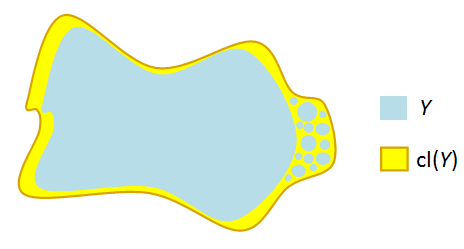
\includegraphics{figures/image_2020-05-26-20-08-04.png}

\end{proof}

\begin{proof}[Variant 2]

\envlist

If \(S\subset X\) is not connected, then there exists a subset
\(A\subset S\) that is both open and closed in the subspace topology,
where \(A\neq \emptyset, S\).

Suppose \(S\) is not connected, then choose \(A\) as above. Then
\(B = S\setminus A\) yields a pair \(A, B\) that disconnects \(S\).
Since \(A\) is closed in \(S\),
\(\mkern 1.5mu\overline{\mkern-1.5muA\mkern-1.5mu}\mkern 1.5mu = A\) and
thus
\(\mkern 1.5mu\overline{\mkern-1.5muA\mkern-1.5mu}\mkern 1.5mu \cap B = A \cap B = \emptyset\).
Similarly, since \(A\) is open, \(B\) is closed, and
\(\mkern 1.5mu\overline{\mkern-1.5muB\mkern-1.5mu}\mkern 1.5mu = B \implies \mkern 1.5mu\overline{\mkern-1.5muB\mkern-1.5mu}\mkern 1.5mu \cap A = B \cap A = \emptyset\).

\end{proof}

\end{solution}

\hypertarget{spring-11-work}{%
\subsubsection{\texorpdfstring{? (Spring '11)
\(\work\)}{? (Spring '11) \textbackslash work}}\label{spring-11-work}}

\begin{problem}[?]

A topological space is \textbf{totally disconnected} if its only
connected subsets are one-point sets.

Is it true that if \(X\) has the discrete topology, it is totally
disconnected?

Is the converse true? Justify your answers.

\end{problem}

\hypertarget{fall-14-work}{%
\subsubsection{\texorpdfstring{21 (Fall '14)
\(\work\)}{21 (Fall '14) \textbackslash work}}\label{fall-14-work}}

\begin{problem}[?]

Let \(X\) and \(Y\) be topological spaces and let \(f : X \to Y\) be a
function.

Suppose that \(X = A \cup B\) where \(A\) and \(B\) are closed subsets,
and that the restrictions \(f \mathrel{\Big|}_A\) and
\(f \mathrel{\Big|}_B\) are continuous (where \(A\) and \(B\) have the
subspace topology).

Prove that \(f\) is continuous.

\end{problem}

\hypertarget{spring-15-done}{%
\subsubsection{\texorpdfstring{23 (Spring '15)
\(\done\)}{23 (Spring '15) \textbackslash done}}\label{spring-15-done}}

\begin{problem}[?]

Define a family \({\mathcal{T}}\) of subsets of \({\mathbb{R}}\) by
saying that \(A \in T\) is \(\iff A = \emptyset\) or
\({\mathbb{R}}\setminus A\) is a finite set.

Prove that \({\mathcal{T}}\) is a topology on \({\mathbb{R}}\), and that
\({\mathbb{R}}\) is compact with respect to this topology.

\end{problem}

\begin{concept}

\envlist

\begin{itemize}
\tightlist
\item
  This is precisely the cofinite topology.
\end{itemize}

\end{concept}

\begin{solution}

\envlist

\begin{enumerate}
\def\labelenumi{\arabic{enumi}.}
\tightlist
\item
  \({\mathbb{R}}\in \tau\) since
  \({\mathbb{R}}\setminus {\mathbb{R}}= \emptyset\) is trivially a
  finite set, and \(\emptyset \in \tau\) by definition.
\item
  If \(U_i \in \tau\) then \((\cup_i U_i)^c = \cap U_i^c\) is an
  intersection of finite sets and thus finite, so
  \(\cup_i U_i \in \tau\).
\item
  If \(U_i \in \tau\), then
  \((\cap_{i=1}^n U_i)^c = \cup_{i=1}^n U_i^c\) is a finite union of
  finite sets and thus finite, so \(\cap U_i \in \tau\).
\end{enumerate}

So \(\tau\) forms a topology.

To see that \(({\mathbb{R}}, \tau)\) is compact, let
\(\left\{{U_i}\right\} \rightrightarrows {\mathbb{R}}\) be an open cover
by elements in \(\tau\).

Fix any \(U_\alpha\), then
\(U_\alpha^c = \left\{{p_1, \cdots, p_n}\right\}\) is finite, say of
size \(n\). So pick \(U_1 \ni p_1, \cdots, U_n \ni p_n\); then
\({\mathbb{R}}\subset U_\alpha \cup_{i=1}^n U_i\) is a finite cover.

\end{solution}

\hypertarget{fall-16-work}{%
\subsubsection{\texorpdfstring{25 (Fall '16)
\(\work\)}{25 (Fall '16) \textbackslash work}}\label{fall-16-work}}

\begin{problem}[?]

Let \({\mathcal{S}}, {\mathcal{T}}\) be topologies on a set \(X\). Show
that \({\mathcal{S}}\cap {\mathcal{T}}\) is a topology on \(X\).

Give an example to show that \({\mathcal{S}}\cup {\mathcal{T}}\) need
not be a topology.

\end{problem}

\hypertarget{spring-10-done-1}{%
\subsubsection{\texorpdfstring{42 (Spring '10)
\(\done\)}{42 (Spring '10) \textbackslash done}}\label{spring-10-done-1}}

\begin{problem}[?]

Define an equivalence relation \(\sim\) on \({\mathbb{R}}\) by
\(x \sim y\) if and only if \(x - y \in {\mathbb{Q}}\). Let \(X\) be the
set of equivalence classes, endowed with the quotient topology induced
by the canonical projection \(\pi : {\mathbb{R}}\to X\).

Describe, with proof, all open subsets of \(X\) with respect to this
topology.

\end{problem}

\hypertarget{fall-12-work}{%
\subsubsection{\texorpdfstring{43 (Fall '12)
\(\work\)}{43 (Fall '12) \textbackslash work}}\label{fall-12-work}}

\begin{problem}[?]

Let \(A\) denote a subset of points of \(S^2\) that looks exactly like
the capital letter A. Let \(Q\) be the quotient of \(S^2\) given by
identifying all points of \(A\) to a single point.

Show that \(Q\) is homeomorphic to a familiar topological space and
identify that space.

\end{problem}

\hypertarget{compactness-and-metric-spaces}{%
\subsection{Compactness and Metric
Spaces}\label{compactness-and-metric-spaces}}

\hypertarget{spring-06-work}{%
\subsubsection{\texorpdfstring{1 (Spring '06)
\(\work\)}{1 (Spring '06) \textbackslash work}}\label{spring-06-work}}

\begin{problem}[?]

Suppose \((X, d)\) is a metric space. State criteria for continuity of a
function \(f : X \to X\) in terms of:

\begin{enumerate}
\def\labelenumi{\roman{enumi}.}
\item
  open sets;
\item
  \(\varepsilon\)'s and \(\delta\)'s; and
\item
  convergent sequences.
\end{enumerate}

Then prove that (iii) implies (i).

\end{problem}

\hypertarget{fall-17-work}{%
\subsubsection{\texorpdfstring{26 (Fall '17)
\(\work\)}{26 (Fall '17) \textbackslash work}}\label{fall-17-work}}

\begin{problem}[?]

Let \(f : X \to Y\) be a continuous function between topological spaces.

Let \(A\) be a subset of \(X\) and let \(f (A)\) be its image in \(Y\) .

One of the following statements is true and one is false. Decide which
is which, prove the true statement, and provide a counterexample to the
false statement:

\begin{enumerate}
\def\labelenumi{\arabic{enumi}.}
\item
  If \(A\) is closed then \(f (A)\) is closed.
\item
  If \(A\) is compact then \(f (A)\) is compact.
\end{enumerate}

\end{problem}

\hypertarget{spring-12-work}{%
\subsubsection{\texorpdfstring{2 (Spring '12)
\(\work\)}{2 (Spring '12) \textbackslash work}}\label{spring-12-work}}

\begin{problem}[?]

Let \(X\) be a topological space.

\begin{enumerate}
\def\labelenumi{\alph{enumi}.}
\item
  State what it means for \(X\) to be compact.
\item
  Let
  \(X = \left\{{0}\right\} \cup \left\{{{1\over n} \mathrel{\Big|}n \in {\mathbb{Z}}^+ }\right\}\).
  Is \(X\) compact?
\item
  Let \(X = (0, 1]\). Is \(X\) compact?
\end{enumerate}

\end{problem}

\todo[inline]{Incomplete proof for part 3.}

\begin{concept}

See Munkres p.164, especially for (ii).

\end{concept}

\begin{solution}

\envlist

\begin{enumerate}
\def\labelenumi{\alph{enumi}.}
\item
  See definitions in review doc.
\item
  Direct proof:
\end{enumerate}

\begin{itemize}
\tightlist
\item
  Let
  \(\left\{{U_i {~\mathrel{\Big|}~}j\in J}\right\}\rightrightarrows X\);
  then \(0\in U_j\) for some \(j\in J\).
\item
  In the subspace topology, \(U_i\) is given by some
  \(V\in \tau({\mathbb{R}})\) such that \(V\cap X = U_i\)

  \begin{itemize}
  \tightlist
  \item
    A basis for the subspace topology on \({\mathbb{R}}\) is open
    intervals, so write \(V\) as a union of open intervals
    \(V = \cup_{k\in K} I_k\).
  \item
    Since \(0\in U_j\), \(0\in I_k\) for some \(k\).
  \end{itemize}
\item
  Since \(I_k\) is an interval, it contains infinitely many points of
  the form \(x_n = {1 \over n} \in X\)
\item
  Then \(I_k \cap X \subset U_j\) contains infinitely many such points.
\item
  So there are only \emph{finitely} many points in \(X\setminus U_j\),
  each of which is in \(U_{j(n)}\) for some \(j(n) \in J\) depending on
  \(n\).
\end{itemize}

\begin{enumerate}
\def\labelenumi{\alph{enumi}.}
\setcounter{enumi}{2}
\tightlist
\item
  Todo
\end{enumerate}

\todo[inline]{Need direct proof}

\end{solution}

\hypertarget{spring-09-work}{%
\subsubsection{\texorpdfstring{3 (Spring '09)
\(\work\)}{3 (Spring '09) \textbackslash work}}\label{spring-09-work}}

\begin{problem}[?]

Let \((X, d)\) be a compact metric space, and let \(f : X \to X\) be an
isometry:
\begin{align*}
\forall~ x, y \in X, \qquad d(f (x), f (y)) = d(x, y)
.\end{align*}
Prove that \(f\) is a bijection.

\end{problem}

\hypertarget{spring-05-done}{%
\subsubsection{\texorpdfstring{4 (Spring '05)
\(\done\)}{4 (Spring '05) \textbackslash done}}\label{spring-05-done}}

\begin{problem}[?]

Suppose \((X, d)\) is a compact metric space and \(U\) is an open
covering of \(X\).

Prove that there is a number \(\delta > 0\) such that for every
\(x \in X\), the ball of radius \(\delta\) centered at \(x\) is
contained in some element of \(U\).

\end{problem}

\begin{solution}

\envlist

Statement: show that the \emph{Lebesgue number} is well-defined for
compact metric spaces.

\begin{quote}
Note: this is a question about the \emph{Lebesgue Number}. See Wikipedia
for detailed proof.
\end{quote}

\begin{itemize}
\tightlist
\item
  Write \(U = \left\{{U_i {~\mathrel{\Big|}~}i\in I}\right\}\), then
  \(X \subseteq \cup_{i\in I} U_i\). Need to construct a \(\delta > 0\).
\item
  By compactness of \(X\), choose a finite subcover
  \(U_1, \cdots, U_n\).
\item
  Define the distance between a point \(x\) and a set \(Y\subset X\):
  \(d(x, Y) = \inf_{y\in Y} d(x, y)\).

  \begin{itemize}
  \tightlist
  \item
    \textbf{Claim}: the function \(d({-}, Y): X\to {\mathbb{R}}\) is
    continuous for a fixed set.
  \item
    Proof: Todo, not obvious.
  \end{itemize}
\end{itemize}

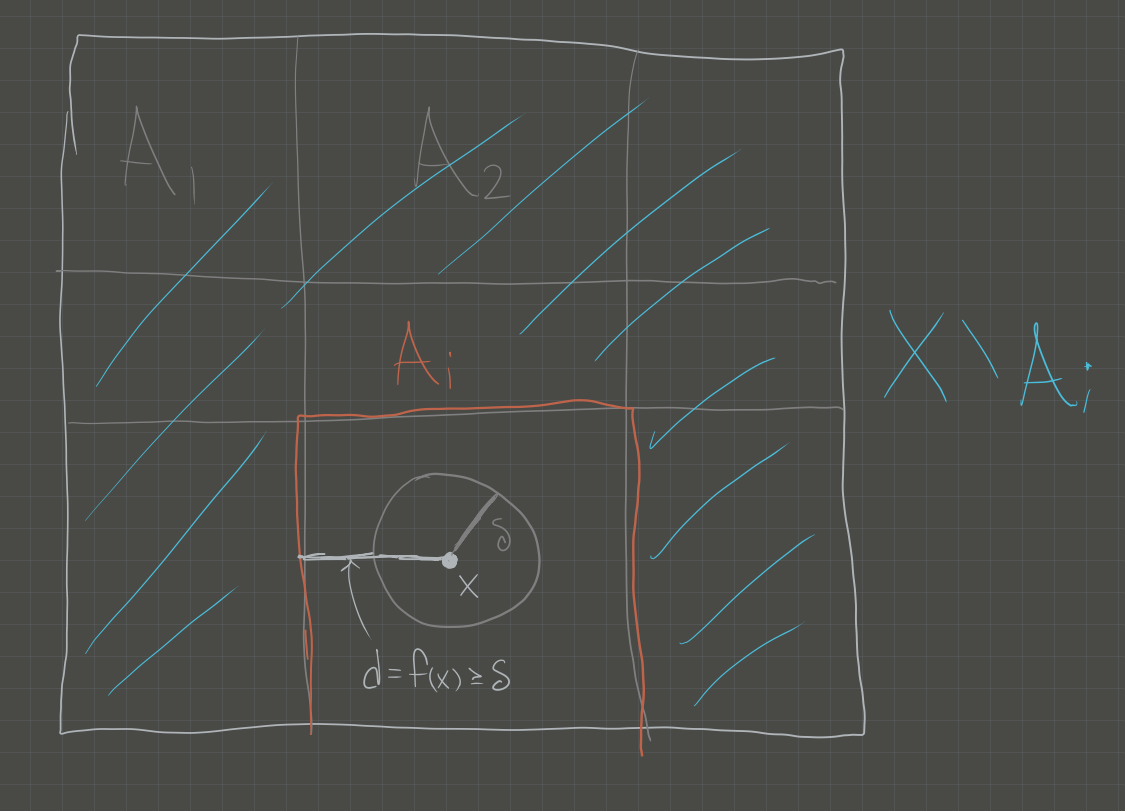
\includegraphics{figures/image_2020-05-22-00-24-45.png}

\begin{itemize}
\tightlist
\item
  Define a function
  \begin{align*}     f: X &\to {\mathbb{R}}\\     x &\mapsto {1\over n} \sum_{i=1}^n d(x, X\setminus U_i)      .\end{align*}

  \begin{itemize}
  \tightlist
  \item
    Note this is a sum of continuous functions and thus continuous.
  \end{itemize}
\item
  \textbf{Claim}:
  \begin{align*}\delta \coloneqq\inf_{x\in X}f(x) = \min_{x\in X}f(x) = f(x_{\text{min}}) > 0\end{align*}
  suffices.

  \begin{itemize}
  \tightlist
  \item
    That the infimum is a minimum: \(f\) is a continuous function on a
    compact set, apply the extreme value theorem: it attains its
    minimum.
  \item
    That \(\delta > 0\): otherwise, \(\delta = 0 \implies \exists x_0\)
    such that \(d(x_0, X\setminus U_i) = 0\) for all \(i\).

    \begin{itemize}
    \tightlist
    \item
      Forces \(x_0 \in X\setminus U_i\) for all \(i\), but
      \(X\setminus \cup U_i = \emptyset\) since the \(U_i\) cover \(X\).
    \end{itemize}
  \item
    That it satisfies the Lebesgue condition:
    \begin{align*}\forall x\in X, \exists i {\quad \operatorname{such that} \quad} B_\delta(x) \subset U_i\end{align*}

    \begin{itemize}
    \tightlist
    \item
      Let \(B_\delta(x) \ni x\); then by minimality
      \(f(x) \geq \delta\).
    \item
      Thus it can \emph{not} be the case that
      \(d(x, X\setminus U_i) < \delta\) for \emph{every} \(i\),
      otherwise
      \begin{align*}f(x) \leq {1\over n}\qty{ \delta + \cdots + \delta} = {n\delta \over n} = \delta\end{align*}
    \item
      So there is some particular \(i\) such that
      \(d(x, X\setminus U_i) \geq \delta\).
    \item
      But then \(B_\delta \subseteq U_i\) as desired.
    \end{itemize}
  \end{itemize}
\end{itemize}

\end{solution}

\hypertarget{spring-15-work}{%
\subsubsection{\texorpdfstring{44 (Spring '15)
\(\work\)}{44 (Spring '15) \textbackslash work}}\label{spring-15-work}}

\begin{problem}[?]

\begin{enumerate}
\def\labelenumi{\alph{enumi}.}
\item
  Prove that a topological space that has a countable base for its
  topology also contains a countable dense subset.
\item
  Prove that the converse to (a) holds if the space is a metric space.
\end{enumerate}

\end{problem}

\hypertarget{fall-07-done}{%
\subsubsection{\texorpdfstring{18 (Fall '07)
\(\done\)}{18 (Fall '07) \textbackslash done}}\label{fall-07-done}}

\begin{problem}[?]

Prove that if \((X, d)\) is a compact metric space, \(f : X \to X\) is a
continuous map, and \(C\) is a constant with \(0 < C < 1\) such that
\begin{align*}
d(f (x), f (y)) \leq C \cdot d(x, y) \quad \forall x, y
,\end{align*}
then \(f\) has a fixed point.

\end{problem}

\begin{solution}

\envlist

\begin{itemize}
\item
  Define a new function
  \begin{align*}     g: X \to {\mathbb{R}}\\     x &\mapsto d_X(x, f(x))     .\end{align*}
\item
  Attempt to minimize. Claim: \(g\) is a continuous function.
\item
  Given claim, a continuous function on a compact space attains its
  infimum, so set
  \begin{align*}       m \coloneqq\inf_{x\in X} g(x)        \end{align*}
  and produce \(x_0\in X\) such that \(g(x) = m\).
\item
  Then
  \begin{align*}     m> 0 \iff d(x_0, f(x_0)) > 0 \iff x_0 \neq f(x_0)     .\end{align*}
\item
  Now apply \(f\) and use the assumption that \(f\) is a contraction to
  contradict minimality of \(m\):
  \begin{align*}     d(f(f(x_0)), f(x_0))      &\leq C\cdot d(f(x_0), x_0) \\      &< d(f(x_0), x_0) \quad\text{since } C<1\\     &\leq m     \end{align*}
\item
  Proof that \(g\) is continuous: use the definition of \(g\), the
  triangle inequality, and that \(f\) is a contraction:
  \begin{align*}     d(x, f(x)) &\leq d(x, y) + d(y, f(y)) + d(f(x), f(y)) \\     \implies d(x, f(x)) - d(y, f(y)) &\leq d(x, y) + d(f(x), f(y)) \\     \implies g(x) - g(y) &\leq d(x, y) + C\cdot d(x, y)  = (C+1) \cdot d(x, y)\\     \end{align*}

  \begin{itemize}
  \tightlist
  \item
    This shows that \(g\) is Lipschitz continuous with constant \(C+1\)
    (implies uniformly continuous, but not used).
  \end{itemize}
\end{itemize}

\end{solution}

\hypertarget{spring-15-done-1}{%
\subsubsection{\texorpdfstring{19 (Spring '15)
\(\done\)}{19 (Spring '15) \textbackslash done}}\label{spring-15-done-1}}

\begin{problem}[?]

Prove that the product of two connected topological spaces is connected.

\end{problem}

\begin{solution}

\envlist

\begin{itemize}
\item
  Use the fact that a union of spaces containing a common point is still
  connected.
\item
  Fix a point \((a, b) \in X \times Y\).
\item
  Since the horizontal slice \(X_b\coloneqq X \times\left\{{b}\right\}\)
  is homeomorphic to \(X\) which is connected, as are all of the
  vertical slices \(Y_x \coloneqq\left\{{x}\right\} \times Y \cong Y\)
  (for any \(x\)), the ``T-shaped'' space \(T_x \coloneqq X_b \cup Y_x\)
  is connected for each \(x\).
\item
  Note that \((a, b) \in T_x\) for every \(x\), so
  \(\cup_{x\in X} T_x = X \times Y\) is connected.
\end{itemize}

\begin{figure}
\centering
\includegraphics{figures/2020-01-21-20:53.png}
\caption{Image}
\end{figure}

\end{solution}

\hypertarget{fall-14-done}{%
\subsubsection{\texorpdfstring{20 (Fall '14)
\(\done\)}{20 (Fall '14) \textbackslash done}}\label{fall-14-done}}

\begin{problem}[?]

\begin{enumerate}
\def\labelenumi{\alph{enumi}.}
\tightlist
\item
\end{enumerate}

Define what it means for a topological space to be:

\begin{enumerate}
\def\labelenumi{\roman{enumi}.}
\item
  \textbf{Connected}
\item
  \textbf{Locally connected}
\end{enumerate}

\begin{enumerate}
\def\labelenumi{\alph{enumi}.}
\setcounter{enumi}{1}
\tightlist
\item
  Give, with proof, an example of a space that is connected but not
  locally connected.
\end{enumerate}

\end{problem}

\todo[inline]{What's the picture?}

\begin{concept}

\envlist

\begin{itemize}
\tightlist
\item
  Consider \({\mathbb{R}}\), unions of intervals, \({\mathbb{Q}}\), and
  the topologists sine curve.
\end{itemize}

\end{concept}

\begin{solution}

\envlist

\begin{proof}[of a]

See definitions in review doc.

\end{proof}

\begin{proof}[of b]

\begin{claim}

\(X\coloneqq\) the Topologist's sine curve suffices.

\end{claim}

\begin{itemize}
\tightlist
\item
  Claim 1: \(X\) is connected.

  \begin{itemize}
  \tightlist
  \item
    Intervals and graphs of cts functions are connected, so the only
    problem point is \(0\).
  \end{itemize}
\item
  Claim 2: \(X\) is \textbf{not} locally connected.

  \begin{itemize}
  \tightlist
  \item
    Take any \(B_\varepsilon(0) \in {\mathbb{R}}^2\); then projecting
    onto the subspace \(\pi_X(B_\varepsilon(0))\) yields infinitely many
    arcs, each intersecting the graph at two points on
    \({{\partial}}B_\varepsilon(0)\).
  \item
    These are homeomorphic to a collection of disjoint embedded open
    intervals, and any disjoint union of intervals is clearly not
    connected.
  \end{itemize}
\end{itemize}

\end{proof}

\end{solution}

\hypertarget{fall-18-work}{%
\subsubsection{\texorpdfstring{22 (Fall '18)
\(\work\)}{22 (Fall '18) \textbackslash work}}\label{fall-18-work}}

\begin{problem}[?]

Let \(X\) be a compact space and let \(f : X \times R \to R\) be a
continuous function such that \(f (x, 0) > 0\) for all \(x \in X\).

Prove that there is \(\varepsilon> 0\) such that \(f (x, t) > 0\)
whenever \({\left\lvert {t} \right\rvert} < \varepsilon\).

Moreover give an example showing that this conclusion may not hold if
\(X\) is not assumed compact.

\end{problem}

\hypertarget{spring-16-work}{%
\subsubsection{\texorpdfstring{24 (Spring '16)
\(\work\)}{24 (Spring '16) \textbackslash work}}\label{spring-16-work}}

\begin{problem}[?]

In each part of this problem \(X\) is a compact topological space. Give
a proof or a counterexample for each statement.

\begin{enumerate}
\def\labelenumi{\alph{enumi}.}
\item
  If \(\left\{{F_n }\right\}_{n=1}^\infty\) is a sequence of nonempty
  \emph{closed} subsets of \(X\) such that \(F_{n+1} \subset F_{n}\) for
  all \(n\) then
  \begin{align*}\cap^\infty_{n=1} F_n\neq \emptyset.\end{align*}
\item
  If \(\left\{{O_n}\right\}_{n=1}^\infty\) is a sequence of nonempty
  \emph{open} subsets of \(X\) such that \(O_{n+1} \subset O_n\) for all
  \(n\) then
  \begin{align*}\cap_{n=1}^\infty O_{n}\neq \emptyset.\end{align*}
\end{enumerate}

\end{problem}

\hypertarget{fall-17-work-1}{%
\subsubsection{\texorpdfstring{27 (Fall '17)
\(\work\)}{27 (Fall '17) \textbackslash work}}\label{fall-17-work-1}}

\begin{problem}[?]

A metric space is said to be \textbf{totally bounded} if for every
\(\varepsilon> 0\) there exists a finite cover of \(X\) by open balls of
radius \(\varepsilon\).

\begin{enumerate}
\def\labelenumi{\alph{enumi}.}
\item
  Show: a metric space \(X\) is totally bounded iff every sequence in
  \(X\) has a Cauchy subsequence.
\item
  Exhibit a complete metric space \(X\) and a closed subset \(A\) of
  \(X\) that is bounded but not totally bounded.
\end{enumerate}

\begin{quote}
You are not required to prove that your example has the stated
properties.
\end{quote}

\end{problem}

\begin{concept}

\envlist

\begin{itemize}
\tightlist
\item
  Use diagonal trick to construct the Cauchy sequence.
\end{itemize}

\end{concept}

\begin{solution}

\envlist

\begin{proof}[of a]

\(\implies\):

If \(X\) is totally bounded, let \(\varepsilon = \frac 1 n\) for each
\(n\), and let \(\left\{{x_i}\right\}\) be an arbitrary sequence. For
\(n=1\), pick a finite open cover \(\left\{{U_i}\right\}_n\) such that
\({\operatorname{diam}}{U_i} < \frac 1 n\) for every \(i\).

Choose \(V_1\) such that there are infinitely many \(x_i \in V_1\).
(Why?) Note that \({\operatorname{diam}}V_i < 1\). Now choose
\(x_i \in V_1\) arbitrarily and define it to be \(y_1\).

Then since \(V_1\) is totally bounded, repeat this process to obtain
\(V_2 \subseteq V_1\) with \({\operatorname{diam}}(V_2)< \frac 1 2\),
and choose \(x_i \in V_2\) arbitrarily and define it to be \(y_2\).

This yields a nested family of sets
\(V_1 \supseteq V_2 \supseteq \cdots\) and a sequence
\(\left\{{y_i}\right\}\) such that
\(d(y_i, y_j) < \max(\frac 1 i, \frac 1 j) \to 0\), so
\(\left\{{y_i}\right\}\) is a Cauchy subsequence.

\(\impliedby\):

Then fix \(\varepsilon > 0\) and pick \(x_1\) arbitrarily and define
\(S_1 = B(\varepsilon, x_1)\). Then pick \(x_2 \in S_1^c\) and define
\(S_2 = S_1 \cup B(\varepsilon, x_2)\), and so on. Continue by picking
\(x_{n+1} \in S_n^c\) (Since \(X\) is not totally bounded, this can
always be done) and defining
\(S_{n+1} = S_n \cup B(\varepsilon, x_{n+1})\).

Then \(\left\{{x_n}\right\}\) is not Cauchy, because
\(d(x_i, x_j) > \varepsilon\) for every \(i\neq j\).

\end{proof}

\begin{proof}[of b]

Take \(X = C^0([0, 1])\) with the sup-norm, then \(f_n(x) = x^n\) are
all bounded by 1, but \({\left\lVert {f_i - f_j} \right\rVert} = 1\) for
every \(i, j\), so no subsequence can be Cauchy, so \(X\) can not be
totally bounded.

Moreover, \(\left\{{f_n}\right\}\) is closed. (Why?)

\end{proof}

\end{solution}

\hypertarget{spring-19-1-done}{%
\subsubsection{\texorpdfstring{Spring '19 \#1
\(\done\)}{Spring '19 \#1 \textbackslash done}}\label{spring-19-1-done}}

\begin{problem}[?]

Is every complete bounded metric space compact? If so, give a proof; if
not, give a counterexample.

\end{problem}

\todo[inline]{Review, from last year.}

\begin{concept}

\envlist

\begin{itemize}
\item
  Complete and \textbf{totally} bounded \(\implies\) compact.
\item
  Definition: A space \(X\) is \emph{totally bounded} if for every
  \(\varepsilon >0\), there is a finite cover
  \(X \subseteq \cup_\alpha B_\alpha(\varepsilon)\) such that the radius
  of each ball is less than \(\varepsilon\).
\item
  Definition: A subset of a space \(S \subset X\) is \emph{bounded} if
  there exists a \(B(r)\) such that \(r<\infty\) and
  \(S \subseteq B(r)\)
\item
  Totally bounded \(\implies\) bounded

  \begin{itemize}
  \tightlist
  \item
    Counterexample to converse: \({\mathbb{N}}\) with the discrete
    metric.
  \item
    Equivalent for Euclidean metric
  \end{itemize}
\item
  Compact \(\implies\) totally bounded.
\item
  Counterexample for problem: the unit ball in any Hilbert (or Banach)
  space of infinite dimension is closed, bounded, and not compact.
\item
  Second counterexample:
  \(({\mathbb{R}}, (x,y) \mapsto \frac{{\left\lvert {x-y} \right\rvert}}{1 + {\left\lvert {x-y} \right\rvert}})\).
\item
  Best counterexample:
  \(X = \left({\mathbb{Z}}, ~\rho ( x , y ) = \left\{ \begin{array} { l l } { 1 } & { \text { if } x \neq y } \\ { 0 } & { \text { if } x = y } \end{array} \right.\right)\).
  This metric makes \(X\) complete for any \(X\), then take
  \({\mathbb{N}}\subset X\). All sets are closed, and bounded, so we
  have a complete, closed, bounded set that is not compact -- take that
  cover \(U_i = B(1, i)\).
\item
  Useful tool: \((X, d) \cong_{\text{Top}} (X, \min{(d(x,y), 1)}\) where
  the RHS is now a bounded space. This preserves all topological
  properties (e.g.~compactness).
\end{itemize}

\end{concept}

\begin{solution}

\envlist

\begin{proof}[?]

Inductively, let \(\mathbf{x}_1 \in B(1, \mathbf{0})\) and
\(A_1 = {\operatorname{span}}{(\mathbf{x}_1)}\), then choose
\(s = \mathbf{x} + A_1 \in B(1,0)/A_1\) such that
\({\left\lVert {s} \right\rVert} = \frac 1 2\) and then a representative
\(\mathbf{x}_2\) such that
\({\left\lVert {\mathbf{x}_2} \right\rVert} \leq 1\). Then
\({\left\lVert {\mathbf{x}_2 - \mathbf{x}_1} \right\rVert} \geq \frac 1 2\)

Then, let \(A_2 = \mathrm{span}(\mathbf{x}_1, \mathbf{x}_2)\), (which is
closed) and repeat this for
\(s = \mathbf{x} + A_2 \in B(1, \mathbf{0})/ A_2\) to get an
\(\mathbf{x}_3\) such that
\({\left\lVert {\mathbf{x}_3 - \mathbf{x}_{\leq 2}} \right\rVert} \geq \frac 1 2\).

This produces a non-convergent sequence in the closed ball, so it can
not be compact.

\end{proof}

\end{solution}

\hypertarget{spring-2019-2-done}{%
\subsubsection{\texorpdfstring{Spring 2019 \#2
\(\done\)}{Spring 2019 \#2 \textbackslash done}}\label{spring-2019-2-done}}

\begin{problem}[?]

Let \(X\) be Hausdorff, and recall that the \emph{one-point
compactification} \(\tilde X\) is given by the following:

\begin{itemize}
\item
  As a set,
  \(\tilde X \coloneqq X{\textstyle\coprod}\left\{{\infty}\right\}\).
\item
  A subset \(U\subseteq \tilde X\) is open iff either \(U\) is open in
  \(X\) or is of the form
  \(U = V{\textstyle\coprod}\left\{{\infty}\right\}\) where
  \(V\subset X\) is arbitrary and \(X\setminus V\) is compact.
\end{itemize}

Prove that this description defines a topology on \(\tilde X\) making
\(\tilde X\) compact.

\end{problem}

\begin{concept}

\envlist

Definition: \((X, \tau)\) where \(\tau \subseteq \mathcal P(X)\) is a
\emph{topological space} iff

\begin{itemize}
\tightlist
\item
  \(\emptyset, X \in \tau\)
\item
  \(\left\{{U_i}\right\}_{i\in I} \subseteq \tau \implies \cup_{i\in I} U_i \in \tau\)
\item
  \(\left\{{U_i}\right\}_{i\in {\mathbb{N}}} \subseteq \tau \implies \cap_{i\in {\mathbb{N}}} U_i \in \tau\)
\end{itemize}

\end{concept}

\begin{solution}

\envlist

We can write
\(\overline{(X, \tau)} = (X {\textstyle\coprod}{\operatorname{pt}}, \tau \cup\tau')\)
where
\(\tau' = \left\{{U{\textstyle\coprod}{\operatorname{pt}}{~\mathrel{\Big|}~}X-U ~\text{is compact}}\right\}\).
We need to show that \(T \coloneqq\tau \cup\tau'\) forms a topology.

\begin{itemize}
\tightlist
\item
  We have
  \(\emptyset,X \in \tau \implies \emptyset, X \in \tau \cup\tau'\).
\item
  We just need to check that \(\tau'\) is closed under arbitrary unions.
  Let \(\left\{{U_i}\right\} \subset \tau'\), so \(X-U_i = K_i\) a
  compact set for each \(i\). Then
  \(\cup_{i} U_i = \cup_i X- (X-U_i)= \cup_i X - K_i = X - \cup_i K_i\)
\end{itemize}

\end{solution}

\hypertarget{spring-2021-3-work}{%
\subsubsection{\texorpdfstring{Spring 2021 \#3
\(\work\)}{Spring 2021 \#3 \textbackslash work}}\label{spring-2021-3-work}}

\begin{problem}[Spring 2021, 3]

For nonempty subsets \(A, B\) of a metric space \((X, d)\), define the
\textbf{setwise distance} as
\begin{align*}
d(A, B) \coloneqq\inf \left\{{ d(a, b) {~\mathrel{\Big|}~}a\in A,\, b\in B }\right\} 
.\end{align*}

\begin{enumerate}
\def\labelenumi{\alph{enumi}.}
\item
  Suppose that \(A\) and \(B\) are compact. Show that there is an
  \(a\in A\) and \(b\in B\) such that \(d(A, B) = d(a, b)\).
\item
  Suppose that \(A\) is closed and \(B\) is compact. Show that if
  \(d(A, B) = 0\) then \(A \cap B = \emptyset\).
\item
  Give an example in which \(A\) is closed, \(B\) is compact, and
  \(d(a, b) > d(A, B)\) for all \(a\in A\) and \(b\in B\).
\end{enumerate}

\begin{quote}
Hint: take \(X = \left\{{ 0 }\right\} \cup(1, 2] \subset {\mathbb{R}}\).
Throughout this problem, you may use without proof that the map
\(d:X\times X\to {\mathbb{R}}\) is continuous.
\end{quote}

\end{problem}

\hypertarget{connectedness}{%
\subsection{Connectedness}\label{connectedness}}

\hypertarget{spring-13-work}{%
\subsubsection{\texorpdfstring{9 (Spring '13)
\(\work\)}{9 (Spring '13) \textbackslash work}}\label{spring-13-work}}

\begin{problem}[?]

Recall that a topological space is said to be \textbf{connected} if
there does not exist a pair \(U, V\) of disjoint nonempty subsets whose
union is \(X\).

\begin{enumerate}
\def\labelenumi{\alph{enumi}.}
\item
  Prove that \(X\) is connected if and only if the only subsets of \(X\)
  that are both open and closed are \(X\) and the empty set.
\item
  Suppose that \(X\) is connected and let \(f : X \to {\mathbb{R}}\) be
  a continuous map. If \(a\) and \(b\) are two points of \(X\) and \(r\)
  is a point of \({\mathbb{R}}\) lying between \(f (a)\) and \(f (b)\)
  show that there exists a point \(c\) of \(X\) such that \(f (c) = r\).
\end{enumerate}

\end{problem}

\hypertarget{fall-05-done-1}{%
\subsubsection{\texorpdfstring{10 (Fall '05)
\(\done\)}{10 (Fall '05) \textbackslash done}}\label{fall-05-done-1}}

\begin{problem}[?]

Let
\begin{align*}
X = \left\{{(0, y) \mathrel{\Big|}- 1 \leq y \leq 1}\right\} \cup \left\{{\qty{x, s = \sin\qty{1 \over x}} \mathrel{\Big|}0 < x \leq 1}\right\}
.\end{align*}

Prove that \(X\) is connected but not path connected.

\end{problem}

\begin{solution}

\envlist

\begin{proof}[Variant 1]

\(X\) is connected:

\begin{itemize}
\tightlist
\item
  Write \(X = L{\textstyle\coprod}G\) where
  \(L = \left\{{0}\right\} \times[-1, 1]\) and
  \(G = \left\{{\Gamma(\sin(x)) {~\mathrel{\Big|}~}x\in (0, 1]}\right\}\)
  is the graph of \(\sin(x)\).
\item
  \(L \cong [0, 1]\) which is connected

  \begin{itemize}
  \tightlist
  \item
    Claim: Every interval is connected (todo)
  \end{itemize}
\item
  Claim: \(G\) is connected (i.e.~as the graph of a continuous function
  on a connected set)

  \begin{itemize}
  \tightlist
  \item
    The function
    \begin{align*}     f: (0, 1] &\to [-1, 1] \\     x &\mapsto \sin(x)     \end{align*}
    is continuous (how to prove?)
  \item
    Products of continuous functions are continuous iff all of the
    components are continuous.
  \item
    Claim: The diagonal map \(\Delta: Y\to Y\times Y\) where
    \(\Delta(t) = (t, t)\) is continuous for any \(Y\) since
    \(\Delta = (\operatorname{id}, \operatorname{id})\)

    \begin{itemize}
    \tightlist
    \item
      Product of identity functions, which are continuous.
    \end{itemize}
  \item
    The composition of continuous function is continuous, therefore
    \begin{align*}     F : (0, 1] &\xrightarrow{\Delta} (0, 1]^2 \xrightarrow{(\operatorname{id}, f)} (0, 1] \times[-1, 1]  \\     t &\mapsto (t, t) \mapsto (t, f(t))     \end{align*}
  \item
    Then \(G = F((0, 1])\) is the continuous image of a connected set
    and thus connected.
  \end{itemize}
\item
  Claim: \(X\) is connected

  \begin{itemize}
  \tightlist
  \item
    Suppose there is a disconnecting cover \(X = A{\textstyle\coprod}B\)
    such that
    \(\mkern 1.5mu\overline{\mkern-1.5muA\mkern-1.5mu}\mkern 1.5mu \cap B = A\cap\mkern 1.5mu\overline{\mkern-1.5muB\mkern-1.5mu}\mkern 1.5mu = \emptyset\)
    and \(A, B \neq \emptyset\).
  \item
    WLOG let \((x, \sin(x))\in B\) for \(x>0\) (otherwise just
    relabeling \(A, B\))
  \item
    Claim: \(B = G\)

    \begin{itemize}
    \tightlist
    \item
      It can't be the case that \(A\) intersects \(G\): otherwise
      \begin{align*}X = A{\textstyle\coprod}B \implies G = (A\cap G) {\textstyle\coprod}(B \cap V)\end{align*}
      disconnects \(G\). So \(A\cap G = \emptyset\), forcing
      \(A \subseteq L\)
    \item
      Similarly \(L\) can not be disconnected, so
      \(B\cap L = \emptyset\) forcing \(B \subset G\)
    \item
      So \(A \subset L\) and \(B\subset G\), and since
      \(X = A{\textstyle\coprod}B\), this forces \(A = L\) and
      \(B = G\).
    \end{itemize}
  \item
    But any open set \(U\) in the subspace topology
    \(L\subset {\mathbb{R}}^2\) (generated by open balls) containing
    \((0, 0) \in L\) is the restriction of a ball
    \(V \subset {\mathbb{R}}^2\) of radius \(r>0\),
    i.e.~\(U = V \cap X\).

    \begin{itemize}
    \tightlist
    \item
      But any such ball contains points of \(G\):
      \begin{align*}n\gg 0 \implies {1 \over n\pi} < r \implies \exists g\in G \text{ s.t. } g\in U.\end{align*}
    \item
      So \(U \cap L \cap G \neq \emptyset\), contradicting
      \(L\cap G = \emptyset\).
    \end{itemize}
  \end{itemize}
\item
  Claim: \(X\) is \emph{not} path-connected.

  \begin{itemize}
  \item
    Todo: ``can't get from \(L\) to \(G\) in finite time''.
  \item
    Toward a contradiction, choose a continuous function \(f:I \to X\)
    with \(f(0) \in G\) and \(f(1) \in L\).

    \begin{itemize}
    \tightlist
    \item
      Since \(L \cong [0, 1]\), use path-connectedness to create a path
      \(f(1) \to (0, 1)\)
    \item
      Concatenate paths and reparameterize to obtain
      \(f(1) = (0, 1) \in L \subset {\mathbb{R}}^2\).
    \end{itemize}
  \item
    Let \(\varepsilon= {1\over 2}\); by continuity there exists a
    \(\delta\in I\) such that
    \begin{align*}
    t\in B_\delta(1) \subset I \implies f(t) \in B_\varepsilon(\mathbf{0}) \in X
    \end{align*}
  \item
    Using the fact that \([1-\delta, 1]\) is connected,
    \(f([1-\delta, 1]) \subset X\) is connected.
  \item
    Let
    \(f(1-\delta) = \mathbf{x}_0 = (x_0, y_0) \subset X\subset {\mathbb{R}}^2\).
  \item
    Define a composite map
    \begin{align*}     F: [0, 1] &\to {\mathbb{R}}     F &\coloneqq{\operatorname{pr}}_{x{\hbox{-}}\text{axis}} \circ f     .\end{align*}

    \begin{itemize}
    \tightlist
    \item
      \(F\) is continuous as a composition of continuous functions.
    \end{itemize}
  \item
    Then \(F([1-\delta, 1]) \subset {\mathbb{R}}\) is connected and thus
    must be an interval \((a, b)\)
  \item
    Since \(f(1) = \mathbf{0}\) which has \(x{\hbox{-}}\)component zero,
    \([0, b] \subset (a, b)\).
  \item
    Since \(f(1-\delta) = \mathbf{x}\), \(F(\mathbf{x}) = x_0\) and this
    \([0, x_0] \subset (a, b)\).
  \item
    Thus for all \(x \in (0, x_0]\) there exists a
    \(t\in [1-\delta, 1]\) such that \(f(t) = (x, \sin\qty{1\over x})\).
  \item
    Now toward the contradiction, choose
    \(x = {1 \over 2n\pi - \pi/2} \in {\mathbb{R}}\) with \(n\) large
    enough such that \(x\in (0, x_0)\).

    \begin{itemize}
    \tightlist
    \item
      Note that \(\sin\qty{1\over x} = -1\) by construction.
    \item
      Apply the previous statement: there exists a \(t\) such that
      \(f(t) = (x, \sin\qty{1\over x}) = (x, -1)\).
    \item
      But then
      \begin{align*}
      {\left\lVert {f(t) - f(x)} \right\rVert} = {\left\lVert {(x, -1) - (0, 1)} \right\rVert} = {\left\lVert {(x, 2)} \right\rVert} > {1\over 2}
      ,\end{align*}
      contradicting continuity of \(f\).
    \end{itemize}
  \end{itemize}
\end{itemize}

\end{proof}

\begin{proof}[Variant 2]

Let \(X = A \cup B\) with
\(A = \left\{{(0, y) {~\mathrel{\Big|}~}y\in [-1, 1] }\right\}\) and
\(B = \left\{{(x, \sin(1/x)) {~\mathrel{\Big|}~}x\in (0, 1]}\right\}\).
Since \(B\) is the graph of a continuous function, which is always
connected. Moreover,
\(X = \mkern 1.5mu\overline{\mkern-1.5muA\mkern-1.5mu}\mkern 1.5mu\),
and the closure of a connected set is still connected.

\begin{proof}[?]

Alternative direct argument: the subspace
\(X' = B \cup\left\{{\mathbf{0}}\right\}\) is not connected. If it were,
write \(X' = U {\textstyle\coprod}V\), where wlog \(\mathbf{0} \in U\).
Then there is an open such that
\(\mathbf{0} \in N_r(\mathbf{0}) \subset U\). But any neighborhood about
zero intersects \(B\), so we must have \(V \subset B\) as a strict
inclusion. But then \(U \cap B\) and \(V\) disconnects \(B\), a
connected set, which is a contradiction.

\end{proof}

To see that \(X\) is not path-connected, suppose toward a contradiction
that there is a continuous function
\(f: I \to X \subset {\mathbb{R}}^2\). In particular, \(f\) is
continuous at \(\mathbf{0}\), and so

\begin{align*} \forall \varepsilon \quad \exists \delta {~\mathrel{\Big|}~}{\left\lVert {\mathbf{x}} \right\rVert} < \delta \implies {\left\lVert {f(\mathbf{x})} \right\rVert} < \varepsilon .\end{align*}

where the norm is the standard Euclidean norm.

However, we can pick \(\varepsilon < 1\), say, and consider points of
the form \(\mathbf{x}_n = (\frac{1}{2n\pi}, 0)\). In particular, we can
pick \(n\) large enough such that
\({\left\lVert {\mathbf{x}_n} \right\rVert}\) is as small as we like,
whereas
\({\left\lVert {f(\mathbf{x}_n)} \right\rVert} = 1 > \varepsilon\) for
all \(n\), a contradiction.

\end{proof}

\end{solution}

\hypertarget{fall-18-work-1}{%
\subsubsection{\texorpdfstring{11 (Fall '18)
\(\work\)}{11 (Fall '18) \textbackslash work}}\label{fall-18-work-1}}

\begin{problem}[?]

Let
\begin{align*} X=\left\{(x, y) \in \mathbb{R}^{2} | x>0, y \geq 0, \text { and } \frac{y}{x} \text { is rational }\right\} \end{align*}
and equip \(X\) with the subspace topology induced by the usual topology
on \({\mathbb{R}}^2\).

Prove or disprove that \(X\) is connected.

\end{problem}

\todo[inline]{Not convincing..}

\begin{solution}

\envlist

\begin{itemize}
\item
  Consider the (continuous) projection
  \(\pi: {\mathbb{R}}^2 \to {\mathbb{RP}}^1\) given by
  \((x, y) \mapsto [y/x, 1]\) in homogeneous coordinates.

  \begin{itemize}
  \tightlist
  \item
    I.e. this sends points to lines through the origin with rational
    slope).
  \end{itemize}
\item
  Note that the image of \(\pi\) is
  \({\mathbb{RP}}^1\setminus\left\{{\infty}\right\}\), which is
  homeomorphic to \({\mathbb{R}}\).
\item
  If we now define \(f = {\left.{{\pi}} \right|_{{X}} }\), we have
  \(f(X) \twoheadrightarrow{\mathbb{Q}}\subset {\mathbb{R}}\).
\item
  If \(X\) were connected, then \(f(X)\) would also be connected, but
  \({\mathbb{Q}}\subset {\mathbb{R}}\) is disconnected, a contradiction.
\end{itemize}

\end{solution}

\hypertarget{spring-2021-2}{%
\subsubsection{Spring 2021 \#2}\label{spring-2021-2}}

\begin{problem}[Spring 2021, 2]

Let \(X \coloneqq\prod_{==1}^{\infty} \left\{{ 0, 1 }\right\}\) endowed
with the product topology.

\begin{enumerate}
\def\labelenumi{\alph{enumi}.}
\item
  Show that for all points \(x,y\in X\) with \(x\neq y\), there are open
  subsets \(U_x, U_y \subset X\) such that \(x\in U_x, y\in U_y\), with
  \(U_x \cup U_y = X\) and \(U_x \cap U_y = \emptyset\).
\item
  Show that \(X\) is totally disconnected, i.e.~the only nonempty
  connected subsets of \(X\) are singletons.
\end{enumerate}

\end{problem}

\hypertarget{hausdorff-spaces-and-separation}{%
\subsection{Hausdorff Spaces and
Separation}\label{hausdorff-spaces-and-separation}}

\hypertarget{fall-14-work-1}{%
\subsubsection{\texorpdfstring{29 (Fall '14)
\(\work\)}{29 (Fall '14) \textbackslash work}}\label{fall-14-work-1}}

\begin{problem}[?]

Is every product (finite or infinite) of Hausdorff spaces Hausdorff? If
yes, prove it. If no, give a counterexample.

\end{problem}

\hypertarget{spring-18-done}{%
\subsubsection{\texorpdfstring{30 (Spring '18)
\(\done\)}{30 (Spring '18) \textbackslash done}}\label{spring-18-done}}

\begin{problem}[?]

Suppose that \(X\) is a Hausdorff topological space and that
\(A \subset X\). Prove that if \(A\) is compact in the subspace topology
then \(A\) is closed as a subset of X.

\end{problem}

\begin{solution}

\envlist

\begin{itemize}
\item
  Let \(A \subset X\) be compact, and pick a fixed
  \(x\in X\setminus A\).
\item
  Since \(X\) is Hausdorff, for arbitrary \(a\in A\), there exists opens
  \(U_{a} \ni a\) and \(U_{x,a}\ni x\) such that
  \(V_{a} \cap U_{x,a} = \emptyset\).
\item
  Then
  \(\left\{{U_{a} {~\mathrel{\Big|}~}a\in A}\right\} \rightrightarrows A\),
  so by compactness there is a finite subcover
  \(\left\{{U_{a_i}}\right\} \rightrightarrows A\).
\item
  Now take \(U = \cup_i U_{a_i}\) and \(V_x = \cap_i V_{a_i, x}\), so
  \(U\cap V = \emptyset\).

  \begin{itemize}
  \tightlist
  \item
    Note that both \(U\) and \(V_x\) are open.
  \end{itemize}
\item
  But then defining \(V \coloneqq\cup_{x\in X\setminus A} V_x\), we have
  \(X\setminus A \subset V\) and \(V\cap A = \emptyset\), so
  \(V = X\setminus A\), which is open and thus \(A\) is closed.
\end{itemize}

\end{solution}

\hypertarget{spring-09-done}{%
\subsubsection{\texorpdfstring{31 (Spring '09)
\(\done\)}{31 (Spring '09) \textbackslash done}}\label{spring-09-done}}

\begin{problem}[Spring 2009, 31]

\envlist

\begin{enumerate}
\def\labelenumi{\alph{enumi}.}
\item
  Show that a continuous bijection from a compact space to a Hausdorff
  space is a homeomorphism.
\item
  Give an example that shows that the ``Hausdorff'' hypothesis in part
  (a) is necessary.
\end{enumerate}

\end{problem}

\begin{concept}

\envlist

\begin{itemize}
\tightlist
\item
  Continuous bijection + open map (or closed map) \(\implies\)
  homeomorphism.
\item
  \textbf{Closed} subsets of compact sets are compact.
\item
  The continuous image of a compact set is compact.
\item
  Compact subsets of Hausdorff spaces are closed.
\end{itemize}

\end{concept}

\begin{solution}

\envlist

\begin{proof}[of a]

We'll show that \(f\) is a closed map.

Let \(U \in X\) be closed.

\begin{itemize}
\tightlist
\item
  Since \(X\) is compact, \(U\) is compact
\item
  Since \(f\) is continuous, \(f(U)\) is compact
\item
  Since \(Y\) is Hausdorff, \(f(U)\) is closed.
\end{itemize}

\end{proof}

\begin{proof}[of b]

Note that any finite space is clearly compact.

Take \(f: ([2], \tau_1) \to ([2], \tau_2)\) to be the identity map,
where \(\tau_1\) is the discrete topology and \(\tau_2\) is the
indiscrete topology. Any map into an indiscrete topology is continuous,
and \(f\) is clearly a bijection.

Let \(g\) be the inverse map; then note that \(1 \in \tau_1\) but
\(g^{-1}(1) = 1\) is not in \(\tau_2\), so \(g\) is not continuous.

\end{proof}

\end{solution}

\hypertarget{fall-14-done-1}{%
\subsubsection{\texorpdfstring{32 (Fall '14)
\(\done\)}{32 (Fall '14) \textbackslash done}}\label{fall-14-done-1}}

\begin{problem}[?]

Let \(X\) be a topological space and let
\begin{align*}
\Delta = \left\{{(x, y) \in X \times X \mathrel{\Big|}x = y}\right\}
.\end{align*}

Show that \(X\) is a Hausdorff space if and only if \(\Delta\) is closed
in \(X \times X\).

\end{problem}

\begin{solution}

\envlist

\(\implies\):

\begin{itemize}
\tightlist
\item
  Let \(p\in X^2\setminus \Delta\).
\item
  Then \(p\) is of the form \((x, y)\) where \(x\neq y\) and
  \(x,y\in X\).
\item
  Since \(X\) is Hausdorff, pick \(N_x, N_y\) in \(X\) such that
  \(N_x \cap N_y = \emptyset\).
\item
  Then \(N_p\coloneqq N_x \times N_y\) is an open set in \(X^2\)
  containing \(p\).
\item
  Claim: \(N_p \cap\Delta = \emptyset\).

  \begin{itemize}
  \tightlist
  \item
    If \(q \in N_p \cap\Delta\), then \(q = (z, z)\) where \(z\in X\),
    and \(q\in N_p \implies q\in N_x \cap N_y = \emptyset\).
  \end{itemize}
\item
  Then \(X^2\setminus \Delta = \cup_p N_p\) is open.
\end{itemize}

\(\impliedby\):

\begin{itemize}
\tightlist
\item
  Let \(x\neq y\in X\).
\item
  Consider \((x, y) \in \Delta^c \subset X^2\), which is open.
\item
  Thus \((x, y) \in B\) for some box in the product topology.
\item
  \(B = U \times V\) where \(U\ni x, V\ni y\) are open in \(X\), and
  \(B \subset X^2\setminus \Delta\).
\item
  Claim: \(U\cap V = \emptyset\).

  \begin{itemize}
  \tightlist
  \item
    Otherwise, \(z\in U\cap V \implies (z, z) \in B\cap\Delta\), but
    \(B \subset X^2\setminus \Delta \implies B \cap\Delta = \emptyset\).
  \end{itemize}
\end{itemize}

\end{solution}

\hypertarget{fall-06-work}{%
\subsubsection{\texorpdfstring{33 (Fall '06)
\(\work\)}{33 (Fall '06) \textbackslash work}}\label{fall-06-work}}

\begin{problem}[?]

If \(f\) is a function from \(X\) to \(Y\) , consider the graph
\begin{align*}
G = \left\{{(x, y) \in X \times Y \mathrel{\Big|}f (x) = y}\right\}
.\end{align*}

\begin{enumerate}
\def\labelenumi{\alph{enumi}.}
\item
  Prove that if \(f\) is continuous and \(Y\) is Hausdorff, then \(G\)
  is a closed subset of \(X \times Y\).
\item
  Prove that if \(G\) is closed and \(Y\) is compact, then \(f\) is
  continuous.
\end{enumerate}

\end{problem}

\hypertarget{fall-04-work}{%
\subsubsection{\texorpdfstring{34 (Fall '04)
\(\work\)}{34 (Fall '04) \textbackslash work}}\label{fall-04-work}}

\begin{problem}[?]

Let X be a noncompact locally compact Hausdorff space, with topology
\({\mathcal{T}}\). Let \(\tilde X = X \cup \left\{{\infty}\right\}\)
(\(X\) with one point adjoined), and consider the family
\({\mathcal{B}}\) of subsets of \(\tilde X\) defined by
\begin{align*}
{\mathcal{B}}= T \cup \left\{{S \cup \left\{{\infty}\right\}\mathrel{\Big|}S \subset X,~~ X \backslash S \text{ is compact}}\right\}
.\end{align*}

\begin{enumerate}
\def\labelenumi{\alph{enumi}.}
\item
  Prove that \({\mathcal{B}}\) is a topology on \(\tilde X\), that the
  resulting space is compact, and that \(X\) is dense in \(\tilde X\).
\item
  Prove that if \(Y \supset X\) is a compact space such that \(X\) is
  dense in \(Y\) and \(Y \backslash X\) is a singleton, then Y is
  homeomorphic to \(\tilde X\).
\end{enumerate}

\begin{quote}
The space \(\tilde X\) is called the \textbf{one-point compactification}
of \(X\).
\end{quote}

\begin{enumerate}
\def\labelenumi{\alph{enumi}.}
\setcounter{enumi}{2}
\item
  Find familiar spaces that are homeomorphic to the one point
  compactifications of
\item
  \(X = (0, 1)\) and
\end{enumerate}

\begin{enumerate}
\def\labelenumi{\roman{enumi}.}
\setcounter{enumi}{1}
\tightlist
\item
  \(X = {\mathbb{R}}^2\).
\end{enumerate}

\end{problem}

\hypertarget{fall-16-work-1}{%
\subsubsection{\texorpdfstring{35 (Fall '16)
\(\work\)}{35 (Fall '16) \textbackslash work}}\label{fall-16-work-1}}

\begin{problem}[?]

Prove that a metric space \(X\) is \textbf{normal}, i.e.~if
\(A, B \subset X\) are closed and disjoint then there exist open sets
\(A \subset U \subset X, ~B \subset V \subset X\) such that
\(U \cap V = \emptyset\).

\end{problem}

\hypertarget{spring-06-work-1}{%
\subsubsection{\texorpdfstring{36 (Spring '06)
\(\work\)}{36 (Spring '06) \textbackslash work}}\label{spring-06-work-1}}

\begin{problem}[?]

Prove that every compact, Hausdorff topological space is normal.

\end{problem}

\hypertarget{spring-09-work-1}{%
\subsubsection{\texorpdfstring{37 (Spring '09)
\(\work\)}{37 (Spring '09) \textbackslash work}}\label{spring-09-work-1}}

\begin{problem}[?]

Show that a connected, normal topological space with more than a single
point is uncountable.

\end{problem}

\hypertarget{spring-08-done}{%
\subsubsection{\texorpdfstring{38 (Spring '08)
\(\done\)}{38 (Spring '08) \textbackslash done}}\label{spring-08-done}}

\begin{problem}[?]

Give an example of a quotient map in which the domain is Hausdorff, but
the quotient is not.

\end{problem}

\begin{solution}

\envlist

\begin{itemize}
\tightlist
\item
  \({\mathbb{R}}\) is clearly Hausdorff, and
  \({\mathbb{R}}/{\mathbb{Q}}\) has the indiscrete topology, and is thus
  non-Hausdorff.
\item
  So take the quotient map
  \(\pi:{\mathbb{R}}\to {\mathbb{R}}/{\mathbb{Q}}\).
\end{itemize}

Direct proof that \({\mathbb{R}}/{\mathbb{Q}}\) isn't Hausdorff:

\begin{itemize}
\tightlist
\item
  Pick
  \([x] \subset U \neq [y] \subset V \in {\mathbb{R}}/{\mathbb{Q}}\) and
  suppose \(U\cap V = \emptyset\).
\item
  Pull back \(U\to A, V\to B\) open disjoint sets in \({\mathbb{R}}\)
\item
  Both \(A, B\) contain intervals, so they contain rationals
  \(p\in A, q\in B\)
\item
  Then \([p] = [q] \in U\cap V\).
\end{itemize}

\end{solution}

\hypertarget{fall-04-work-1}{%
\subsubsection{\texorpdfstring{39 (Fall '04)
\(\work\)}{39 (Fall '04) \textbackslash work}}\label{fall-04-work-1}}

\begin{problem}[?]

Let \(X\) be a compact Hausdorff space and suppose
\(R \subset X \times X\) is a closed equivalence relation. Show that the
quotient space \(X/R\) is Hausdorff.

\end{problem}

\hypertarget{spring-18-work}{%
\subsubsection{\texorpdfstring{40 (Spring '18)
\(\work\)}{40 (Spring '18) \textbackslash work}}\label{spring-18-work}}

\begin{problem}[?]

Let \(U \subset {\mathbb{R}}^n\) be an open set which is bounded in the
standard Euclidean metric. Prove that the quotient space
\({\mathbb{R}}^n / U\) is not Hausdorff.

\end{problem}

\hypertarget{fall-09-work}{%
\subsubsection{\texorpdfstring{41 (Fall '09)
\(\work\)}{41 (Fall '09) \textbackslash work}}\label{fall-09-work}}

\begin{problem}[?]

Let \(A\) be a closed subset of a normal topological space \(X\). Show
that both \(A\) and the quotient \(X/A\) are normal.

\end{problem}

\hypertarget{spring-11-work-1}{%
\subsubsection{\texorpdfstring{45 (Spring '11)
\(\work\)}{45 (Spring '11) \textbackslash work}}\label{spring-11-work-1}}

\begin{problem}[?]

Recall that a topological space is \textbf{regular} if for every point
\(p \in X\) and for every closed subset \(F \subset X\) not containing
\(p\), there exist disjoint open sets \(U, V \subset X\) with
\(p \in U\) and \(F \subset V\).

Let \(X\) be a regular space that has a countable basis for its
topology, and let \(U\) be an open subset of \(X\).

\begin{enumerate}
\def\labelenumi{\alph{enumi}.}
\item
  Show that \(U\) is a countable union of closed subsets of \(X\).
\item
  Show that there is a continuous function \(f : X \to [0,1]\) such that
  \(f (x) > 0\) for \(x \in U\) and \(f (x) = 0\) for \(x \in U\).
\end{enumerate}

\end{problem}

\hypertarget{exercises}{%
\subsection{Exercises}\label{exercises}}

\hypertarget{basics}{%
\subsubsection{Basics}\label{basics}}

\hypertarget{exercise-work}{%
\paragraph{\texorpdfstring{Exercise
\(\work\)}{Exercise \textbackslash work}}\label{exercise-work}}

Show that for \(A\subseteq X\), \({ \operatorname{cl}} _X(A)\) is the
smallest closed subset containing \(A\).

\hypertarget{exercise-done}{%
\paragraph{\texorpdfstring{Exercise
\(\done\)}{Exercise \textbackslash done}}\label{exercise-done}}

Give an example of spaces \(A\subseteq B \subseteq X\) such that \(A\)
is open in \(B\) but \(A\) is \emph{not} open in \(X\).

\begin{solution}

\hfill

\begin{concept}

\hfill

\end{concept}

No: Take \([0, 1] \subset [0, 1] \subset {\mathbb{R}}\). Then \([0, 1]\)
is tautologically open in \([0, 1]\) as it is the entire space, But
\([0, 1]\) is not open in \({\mathbb{R}}\): - E.g.
\(\left\{{1}\right\}\) is not an interior point (every neighborhood
intersects the complement \({\mathbb{R}}\setminus[0, 1]\)).

\end{solution}

\hypertarget{exercise-work-1}{%
\paragraph{\texorpdfstring{Exercise
\(\work\)}{Exercise \textbackslash work}}\label{exercise-work-1}}

Show that the diagonal map \(\Delta(x) = (x, x)\) is continuous.

\hypertarget{exercise-work-2}{%
\paragraph{\texorpdfstring{Exercise
\(\work\)}{Exercise \textbackslash work}}\label{exercise-work-2}}

Show that if \(A_i \subseteq X\), then
\({ \operatorname{cl}} _X(\cup_i A_i) = \cup_i { \operatorname{cl}} _X(A_i)\).

\hypertarget{exercise-work-3}{%
\paragraph{\texorpdfstring{Exercise
\(\work\)}{Exercise \textbackslash work}}\label{exercise-work-3}}

Show that \({\mathbb{R}}\) is not homeomorphic to \([0, \infty)\).

\hypertarget{exercise-work-4}{%
\paragraph{\texorpdfstring{Exercise
\(\work\)}{Exercise \textbackslash work}}\label{exercise-work-4}}

Show that the set \((x, y) \in {\mathbb{R}}^2\) such that at least one
of \(x, y\) is rational with the subspace topology is a connected space.

\hypertarget{exercise-mathbbrmathbbq-is-indiscrete}{%
\paragraph{\texorpdfstring{Exercise: \({\mathbb{R}}/{\mathbb{Q}}\) is
indiscrete}{Exercise: \{\textbackslash mathbb\{R\}\}/\{\textbackslash mathbb\{Q\}\} is indiscrete}}\label{exercise-mathbbrmathbbq-is-indiscrete}}

\begin{problem}[?]

Show that \({\mathbb{R}}/{\mathbb{Q}}\) has the indiscrete topology.

\end{problem}

\begin{solution}

\envlist

\begin{itemize}
\tightlist
\item
  Let \(U \subset {\mathbb{R}}/{\mathbb{Q}}\) be open and nonempty, show
  \(U = {\mathbb{R}}/{\mathbb{Q}}\).
\item
  Let \([x] \in U\), then
  \(x \in \pi^{-1}(U) \coloneqq V \subset{\mathbb{R}}\) is open.
\item
  Then \(V\) contains an interval \((a, b)\)
\item
  Every \(y\in V\) satisfies \(y+q \in V\) for all
  \(q\in {\mathbb{Q}}\), since
  \(y+q-y \in {\mathbb{Q}}\implies [y+q] = [y]\).
\item
  So \((a-q, b+q) \in V\) for all \(q\in {\mathbb{Q}}\).
\item
  So
  \(\cup_{q\in {\mathbb{Q}}}(a-q, b+q) \in V \implies {\mathbb{R}}\subset V\).
\item
  So \(\pi(V) = {\mathbb{R}}/{\mathbb{Q}}= U\), and thus the only open
  sets are the entire space and the empty set.
\end{itemize}

\end{solution}

\hypertarget{connectedness-1}{%
\subsubsection{Connectedness}\label{connectedness-1}}

\hypertarget{exercise-work-5}{%
\paragraph{\texorpdfstring{Exercise
\(\work\)}{Exercise \textbackslash work}}\label{exercise-work-5}}

Prove that \(X\) is connected iff the only clopen subsets are
\(\emptyset, X\).

\hypertarget{exercise-work-6}{%
\paragraph{\texorpdfstring{Exercise
\(\work\)}{Exercise \textbackslash work}}\label{exercise-work-6}}

Let \(A \subset X\) be a connected subspace.

Show that if \(B\subset X\) satisfies
\(A\subseteq B \subseteq \mkern 1.5mu\overline{\mkern-1.5muA\mkern-1.5mu}\mkern 1.5mu\),
then \(B\) is connected.

\hypertarget{exercise-work-7}{%
\paragraph{\texorpdfstring{Exercise
\(\work\)}{Exercise \textbackslash work}}\label{exercise-work-7}}

Show that: - Connected does not imply path connected - Connected and
locally path connected \emph{does} imply path connected - Path connected
implies connected

\hypertarget{exercise-work-8}{%
\paragraph{\texorpdfstring{Exercise
\(\work\)}{Exercise \textbackslash work}}\label{exercise-work-8}}

Use the fact that intervals are connected to prove the intermediate
value theorem.

\hypertarget{exercise-work-9}{%
\paragraph{\texorpdfstring{Exercise
\(\work\)}{Exercise \textbackslash work}}\label{exercise-work-9}}

Prove that the continuous image of a connected set is connected.

\hypertarget{exercise-work-10}{%
\paragraph{\texorpdfstring{Exercise
\(\work\)}{Exercise \textbackslash work}}\label{exercise-work-10}}

Show that if \(X\) is locally path connected, then

\begin{itemize}
\tightlist
\item
  Every open subset of \(X\) is again locally path-connected.
\item
  \(X\) is connected \(\iff X\) is path-connected.
\item
  Every path component of \(X\) is a connected component of \(X\).
\item
  Every connected component of \(X\) is open in \(X\).
\end{itemize}

\hypertarget{exercise-done-1}{%
\paragraph{\texorpdfstring{Exercise
\(\done\)}{Exercise \textbackslash done}}\label{exercise-done-1}}

Show that \([0, 1]\) is connected.

\begin{solution}

\hfill

\begin{concept}

\hfill [Reference](https://sites.math.washington.edu/\textasciitilde morrow/334\_16/connected.pdf)
\href{https://math.stackexchange.com/questions/934421/proof-of-that-every-interval-is-connected}{A
potentially shorter proof}

\end{concept}

Let \(I = [0, 1] = A\cup B\) be a disconnection, so -
\(A, B \neq \emptyset\) - \(A {\textstyle\coprod}B = I\) -
\({ \operatorname{cl}} _I(A) \cap B = A \cap{ \operatorname{cl}} _I(B) = \emptyset\).
Let \(a\in A\) and \(b\in B\) where WLOG \(a<b\) - (since either \(a<b\)
or \(b<a\), and \(a\neq b\) since \(A, B\) are disjoint) Let
\(K = [a, b]\) and define \(A_K \coloneqq A\cap K\) and
\(B_K \coloneqq B\cap K\). Now \(A_K, B_K\) is a disconnection of \(K\).
Let \(s = \sup(A_K)\), which exists since \({\mathbb{R}}\) is complete
and has the LUB property Claim: \(s \in { \operatorname{cl}} _I(A_K)\).
Proof: - If \(s\in A_K\) there's nothing to show since
\(A_K \subset { \operatorname{cl}} _I(A_K)\), so assume
\(s\in I\setminus A_K\). - Now let \(N_s\) be an arbitrary neighborhood
of \(s\), then using ??? we can find an \(\varepsilon>0\) such that
\(B_\varepsilon(s) \subset N_s\) - Since \(s\) is a supremum, there
exists an \(a\in A_K\) such that \(s-\varepsilon< a\). - But then
\(a \in B_\varepsilon(s)\) and \(a\in N_s\) with \(a\neq s\). - Since
\(N_s\) was arbitrary, every \(N_s\) contains a point of \(A_K\) not
equal to \(s\), so \(s\) is a limit point by definition. Since
\(s\in { \operatorname{cl}} _I(A_K)\) and
\({ \operatorname{cl}} _I(A_K)\cap B_K = \emptyset\), we have
\(s\not \in B_K\). Then the subinterval \((x, b] \cap A_K = \emptyset\)
for every \(x>c\) since \(c \coloneqq\sup A_K\). But since
\(A_K {\textstyle\coprod}B_K = K\), we must have \((x, b] \subset B_K\),
and thus \(s\in { \operatorname{cl}} _I(B_K)\). Since \(A_K, B_K\) were
assumed disconnecting, \(s\not \in A_K\) But then \(s\in K\) but
\(s\not\in A_K {\textstyle\coprod}B_K = K\), a contradiction.

\end{solution}

\hypertarget{compactness}{%
\subsubsection{Compactness}\label{compactness}}

\hypertarget{star-exercise-done}{%
\paragraph{\texorpdfstring{\(\star\) Exercise
\(\done\)}{\textbackslash star Exercise \textbackslash done}}\label{star-exercise-done}}

Let \(X\) be a compact space and let \(A\) be a closed subspace. Show
that \(A\) is compact.

\begin{solution}

\hfill

\begin{concept}

\hfill

\end{concept}

Let \(X\) be compact, \(A\subset X\) closed, and
\(\left\{{U_\alpha}\right\} \rightrightarrows A\) be an open cover. By
definition of the subspace topology, each \(U_\alpha = V_\alpha \cap A\)
for some open \(V_\alpha \subset X\), and
\(A\subset \cup_\alpha V_\alpha\). Since \(A\) is closed in \(X\),
\(X\setminus A\) is open. Then
\(\left\{{V_\alpha}\right\}\cup\left\{{X\setminus A}\right\}\rightrightarrows X\)
is an open cover, since every point is either in \(A\) or
\(X\setminus A\). By compactness of \(X\), there is a finite subcover
\(\left\{{U_j {~\mathrel{\Big|}~}j\leq N}\right\}\cup\left\{{X\setminus A}\right\}\)
Then
\(\qty{\left\{{U_j}\right\} \cup\left\{{X\setminus A}\right\}} \cap A \coloneqq\left\{{V_j}\right\}\)
is a finite cover of \(A\).

\end{solution}

\hypertarget{star-exercise-done-1}{%
\paragraph{\texorpdfstring{\(\star\) Exercise
\(\done\)}{\textbackslash star Exercise \textbackslash done}}\label{star-exercise-done-1}}

Let \(f : X \to Y\) be a continuous function, with \(X\) compact. Show
that \(f(X)\) is compact.

\begin{solution}

\hfill

\begin{concept}

\hfill

\end{concept}

Let \(f:X\to Y\) be continuous with \(X\) compact, and
\(\left\{{U_\alpha}\right\} \rightrightarrows f(X)\) be an open cover.
Then \(\left\{{f^{-1}(U_\alpha)}\right\} \rightrightarrows X\) is an
open cover of \(X\), since
\(x\in X \implies f(x) \in f(X) \implies f(x) \in U_\alpha\) for some
\(\alpha\), so \(x\in f^{-1}(U_\alpha)\) by definition. By compactness
of \(X\) there is a finite subcover
\(\left\{{f^{-1}(U_j) {~\mathrel{\Big|}~}j\leq N}\right\} \rightrightarrows X\).
Then the finite subcover
\(\left\{{U_j{~\mathrel{\Big|}~}j\leq N}\right\} \rightrightarrows f(X)\),
since if \(y\in f(X)\), \(y\in U_\alpha\) for some \(\alpha\) and thus
\(f^{-1}(y) \in f^{-1}(U_j)\) for some \(j\) since
\(\left\{{U_j}\right\}\) is a cover of \(X\).

\end{solution}

Let \(A\) be a compact subspace of a Hausdorff space \(X\). Show that
\(A\) is closed.

\hypertarget{exercise-work-11}{%
\paragraph{\texorpdfstring{Exercise
\(\work\)}{Exercise \textbackslash work}}\label{exercise-work-11}}

Show that any infinite set with the cofinite topology is compact.

\hypertarget{exercise-work-12}{%
\paragraph{\texorpdfstring{Exercise
\(\work\)}{Exercise \textbackslash work}}\label{exercise-work-12}}

Show that every compact metric space is complete.

\hypertarget{exercise-work-13}{%
\paragraph{\texorpdfstring{Exercise
\(\work\)}{Exercise \textbackslash work}}\label{exercise-work-13}}

Show that if \(X\) is second countable and Hausdorff, or a metric space,
then TFAE:

\begin{itemize}
\tightlist
\item
  \(X\) is compact
\item
  Every infinite subset \(A\subseteq X\) has a limit point in \(X\).
\item
  Every sequence in \(X\) has a convergent subsequence in \(X\).
\end{itemize}

\hypertarget{exercise-work-14}{%
\paragraph{\texorpdfstring{Exercise
\(\work\)}{Exercise \textbackslash work}}\label{exercise-work-14}}

Show that if \(f: A\to B\) is a continuous map between metric spaces and
\(K\subset A\) is compact, then \({\left.{{f}} \right|_{{K}} }\) is
uniformly continuous.

\hypertarget{exercise-work-15}{%
\paragraph{\texorpdfstring{Exercise
\(\work\)}{Exercise \textbackslash work}}\label{exercise-work-15}}

Show that if \(f:X\to Y\) is continuous and \(X\) is compact then
\(f(X)\) is compact.

\hypertarget{exercise-work-16}{%
\paragraph{\texorpdfstring{Exercise
\(\work\)}{Exercise \textbackslash work}}\label{exercise-work-16}}

Show that if \(f:X\to {\mathbb{R}}\) and \(X\) is compact then \(f\) is
bounded and attains its min/max.

\hypertarget{exercise-work-17}{%
\paragraph{\texorpdfstring{Exercise
\(\work\)}{Exercise \textbackslash work}}\label{exercise-work-17}}

Show that a finite product or union compact spaces is again compact.

\hypertarget{exercise-work-18}{%
\paragraph{\texorpdfstring{Exercise
\(\work\)}{Exercise \textbackslash work}}\label{exercise-work-18}}

Show that a quotient of a compact space is again compact.

\hypertarget{exercise-work-19}{%
\paragraph{\texorpdfstring{Exercise
\(\work\)}{Exercise \textbackslash work}}\label{exercise-work-19}}

Show that if \(X\) is compact and \(A\subseteq X\) is closed then \(A\)
is compact.

\hypertarget{exercise-work-20}{%
\paragraph{\texorpdfstring{Exercise
\(\work\)}{Exercise \textbackslash work}}\label{exercise-work-20}}

Show that if \(X\) is Hausdorff and \(A\subseteq X\) is compact then
\(A\) is closed.

\hypertarget{exercise-work-21}{%
\paragraph{\texorpdfstring{Exercise
\(\work\)}{Exercise \textbackslash work}}\label{exercise-work-21}}

Show that if \(X\) is a metric space and \(A\subseteq X\) is compact
then \(A\) is bounded.

\hypertarget{exercise-work-22}{%
\paragraph{\texorpdfstring{Exercise
\(\work\)}{Exercise \textbackslash work}}\label{exercise-work-22}}

Show that a continuous map from a compact space to a Hausdorff space is
closed.

\hypertarget{exercise-work-23}{%
\paragraph{\texorpdfstring{Exercise
\(\work\)}{Exercise \textbackslash work}}\label{exercise-work-23}}

Show that an injective continuous map from a compact space to a
Hausdorff space is an embedding (a homeomorphism onto its image).

\hypertarget{exercise-work-24}{%
\paragraph{\texorpdfstring{Exercise
\(\work\)}{Exercise \textbackslash work}}\label{exercise-work-24}}

Show that \([0, 1]\) is compact.

\hypertarget{exercise-work-25}{%
\paragraph{\texorpdfstring{Exercise
\(\work\)}{Exercise \textbackslash work}}\label{exercise-work-25}}

Show that a compact Hausdorff space is is metrizable iff it is
second-countable.

\hypertarget{exercise-work-26}{%
\paragraph{\texorpdfstring{Exercise
\(\work\)}{Exercise \textbackslash work}}\label{exercise-work-26}}

Show that if \(X\) is metrizable, then \(X\) is compact

\hypertarget{exercise-work-27}{%
\paragraph{\texorpdfstring{Exercise
\(\work\)}{Exercise \textbackslash work}}\label{exercise-work-27}}

Give an example of a space that is compact but not sequentially compact,
and vice versa.

\hypertarget{exercise-work-28}{%
\paragraph{\texorpdfstring{Exercise
\(\work\)}{Exercise \textbackslash work}}\label{exercise-work-28}}

Show that a sequentially compact space is totally bounded.

\hypertarget{exercise-work-29}{%
\paragraph{\texorpdfstring{Exercise
\(\work\)}{Exercise \textbackslash work}}\label{exercise-work-29}}

Show that \({\mathbb{R}}\) with the cofinite topology is compact.

\hypertarget{exercise-work-30}{%
\paragraph{\texorpdfstring{Exercise
\(\work\)}{Exercise \textbackslash work}}\label{exercise-work-30}}

Show that \([0, 1]\) is compact without using the Heine-Borel theorem.

\hypertarget{separation}{%
\subsubsection{Separation}\label{separation}}

\hypertarget{exercise-work-31}{%
\paragraph{\texorpdfstring{Exercise
\(\work\)}{Exercise \textbackslash work}}\label{exercise-work-31}}

Show that \(X\) is Hausdorff iff \(\Delta(X)\) is closed in
\(X\times X\).

\hypertarget{exercise-work-32}{%
\paragraph{\texorpdfstring{Exercise
\(\work\)}{Exercise \textbackslash work}}\label{exercise-work-32}}

Prove that \(X, Y\) are Hausdorff iff \(X\times Y\) is Hausdorff.

\hypertarget{exercise-work-33}{%
\paragraph{\texorpdfstring{Exercise
\(\work\)}{Exercise \textbackslash work}}\label{exercise-work-33}}

Show that \({\mathbb{R}}\) is separable.

\hypertarget{exercise-work-34}{%
\paragraph{\texorpdfstring{Exercise
\(\work\)}{Exercise \textbackslash work}}\label{exercise-work-34}}

Show that any space with the indiscrete topology is separable.

\hypertarget{exercise-work-35}{%
\paragraph{\texorpdfstring{Exercise
\(\work\)}{Exercise \textbackslash work}}\label{exercise-work-35}}

Show that any countable space with the discrete topology is separable.

\hypertarget{exercise-work-36}{%
\paragraph{\texorpdfstring{Exercise
\(\work\)}{Exercise \textbackslash work}}\label{exercise-work-36}}

Show that the minimal uncountable order with the order topology is not
separable.

\hypertarget{exercise-work-37}{%
\paragraph{\texorpdfstring{Exercise
\(\work\)}{Exercise \textbackslash work}}\label{exercise-work-37}}

Show that every first countable space is second countable.

\hypertarget{exercise-work-38}{%
\paragraph{\texorpdfstring{Exercise
\(\work\)}{Exercise \textbackslash work}}\label{exercise-work-38}}

Show that every metric space is Hausdorff in its metric topology.

\hypertarget{hausdorff-spaces}{%
\subsubsection{Hausdorff Spaces}\label{hausdorff-spaces}}

\hypertarget{exercise}{%
\paragraph{Exercise}\label{exercise}}

Show that a compact set in a Hausdorff space is closed.

\hypertarget{exercise-done-2}{%
\paragraph{\texorpdfstring{Exercise
\(\done\)}{Exercise \textbackslash done}}\label{exercise-done-2}}

Let \(A\subset X\) with \(A\) closed and \(X\) compact, and show that
\(A\) is compact.

\begin{concept}

Alternative definition of ``open'': todo.

\end{concept}

\begin{solution}

\envlist

\begin{itemize}
\tightlist
\item
  Let \(A\) be a compact subset of \(X\) a Hausdorff space, we will show
  \(X\setminus A\) is open
\item
  Fix \(x\in X\setminus A\).
\item
  Since \(X\) is Hausdorff, for every \(y\in A\) we can find
  \(U_y \ni y\) and \(V_x(y) \ni x\) depending on \(y\) such that
  \(U_x(y) \cap U_y = \emptyset\).
\item
  Then
  \(\left\{{U_y {~\mathrel{\Big|}~}y\in A}\right\} \rightrightarrows A\),
  and by compactness of \(A\) there is a finite subcover corresponding
  to a finite collection \(\left\{{y_1, \cdots, y_n}\right\}\).
\item
  \textbf{Magic Step}: set \(U = \cup U_{y_i}\) and
  \(V = \cap V_x(y_i)\);

  \begin{itemize}
  \tightlist
  \item
    Note \(A\subset U\) and \(x\in V\)
  \item
    Note \(U\cap V = \emptyset\).
  \end{itemize}
\item
  Done: for every \(x\in X\setminus A\), we have found an open set
  \(V\ni x\) such that \(V\cap A = \emptyset\), so \(x\) is an interior
  point and a set is open iff every point is an interior point.
\end{itemize}

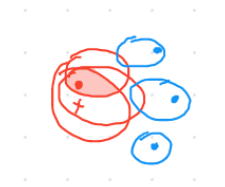
\includegraphics{figures/image_2020-06-11-20-14-26.png}

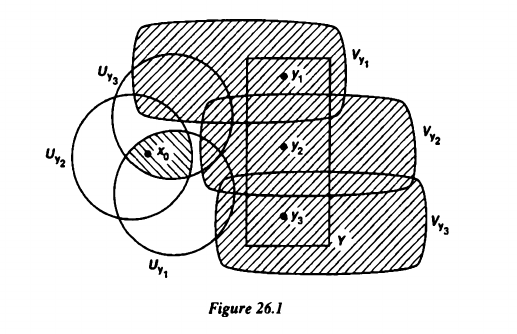
\includegraphics{figures/image_2020-06-11-20-35-11.png}

\end{solution}

\hypertarget{exercise-done-3}{%
\paragraph{\texorpdfstring{Exercise
\(\done\)}{Exercise \textbackslash done}}\label{exercise-done-3}}

Show that a continuous bijection from a compact space to a Hausdorff
space is a homeomorphism.

\begin{solution}

\envlist

\begin{itemize}
\tightlist
\item
  It suffices to show that \(f\) is a closed map, i.e.~if
  \(U\subseteq X\) is closed then \(f(U)\subseteq Y\) is again closed.
\item
  Let \(U\in X\) be closed; since \(X\) is closed, \(U\) is compact

  \begin{itemize}
  \tightlist
  \item
    Since closed subsets of compact spaces are compact.
  \end{itemize}
\item
  Since \(f\) is continuous, \(f(U)\) is compact

  \begin{itemize}
  \tightlist
  \item
    Since the continuous image of a compact set is compact.
  \end{itemize}
\item
  Since \(Y\) is Hausdorff and \(f(U)\) is compact, \(f(U)\) is closed

  \begin{itemize}
  \tightlist
  \item
    Since compact subsets of Hausdorff spaces are closed.
  \end{itemize}
\end{itemize}

\end{solution}

\hypertarget{exercise-work-39}{%
\paragraph{\texorpdfstring{Exercise
\(\work\)}{Exercise \textbackslash work}}\label{exercise-work-39}}

Show that a closed subset of a Hausdorff space need not be compact.

\hypertarget{exercise-work-40}{%
\paragraph{\texorpdfstring{Exercise
\(\work\)}{Exercise \textbackslash work}}\label{exercise-work-40}}

Show that in a \emph{compact} Hausdorff space, \(A\) is closed iff \(A\)
is compact.

\hypertarget{exercise-work-41}{%
\paragraph{\texorpdfstring{Exercise
\(\work\)}{Exercise \textbackslash work}}\label{exercise-work-41}}

Show that a local homeomorphism between compact Hausdorff spaces is a
covering space.

\hypertarget{the-fundamental-group}{%
\section{The Fundamental Group}\label{the-fundamental-group}}

\hypertarget{spring-15-done-2}{%
\subsection{\texorpdfstring{1 (Spring '15)
\(\done\)}{1 (Spring '15) \textbackslash done}}\label{spring-15-done-2}}

\begin{problem}[?]

Let \(S^1\) denote the unit circle in \(C\), \(X\) be any topological
space, \(x_0 \in X\), and
\begin{align*}\gamma_0, \gamma_1 : S^1 \to X\end{align*}
be two continuous maps such that \(\gamma_0 (1) = \gamma_1 (1) = x_0\).

Prove that \(\gamma_0\) is homotopic to \(\gamma_1\) if and only if the
elements represented by \(\gamma_0\) and \(\gamma_1\) in
\(\pi_1 (X, x_0 )\) are conjugate.

\end{problem}

\begin{concept}

\envlist

\begin{itemize}
\tightlist
\item
  Any two maps \(f_i: Y\to X\) are \textbf{homotopic} iff there exists a
  homotopy \(H: I\times Y \to X\) with \(H_0 = f_0\) and \(H_1 = f_1\).
\item
  \(\pi_1(X; x_0)\) is the set of maps \(f:S^1\to X\) such that
  \(f(0) = f(1) = x_0\), modulo being homotopic maps.
\item
  Loops can be homotopic (i.e.~\emph{freely} homotopic) without being
  homotopic rel a base point, so not equal in \(\pi_1(X; x_0)\).

  \begin{itemize}
  \tightlist
  \item
    Counterexample where homotopic loops are not equal in \(\pi_1\), but
    just conjugate. Need nonabelian \(\pi_1\) for conjugates to possibly
    not be equal, so take a torus:
  \end{itemize}

  \includegraphics{figures/2020-02-04-20:00.png}\\
\end{itemize}

\end{concept}

\begin{solution}

\hfill

\(\implies\):

\begin{itemize}
\tightlist
\item
  Suppose \(\gamma_1 \simeq\gamma_2\), then there exists a free homotopy
  \(H: I\times S^1 \to X\) with \(H_0 = \gamma_0, H_1 = \gamma_1\).
\item
  Since \(H(0, 1) \gamma_0(1) = x_0\) and
  \(H(1, 1) = \gamma_1(1) = x_0\), the map
  \begin{align*}
  T: [0, 1] &\to X \\
  t &\mapsto H(t, 1)
  \end{align*}
  descends to a loop \(T:S^1\to X\).
\item
  Claim: \(\gamma_1\) and \(T\ast \gamma_2 \ast T^{-1}\) are homotopic
  rel \(x_0\), making \(\gamma_1, \gamma_2\) conjugate in \(\pi_1\).

  \begin{itemize}
  \tightlist
  \item
    Idea: for each fixed \(s\), follow \(T\) for the first third,
    \(\gamma_2\) for the middle third, \(T^{-1}\) for the last third.
  \end{itemize}

  \includegraphics{figures/2020-02-04-20:23.png}
\end{itemize}

\(\impliedby\):

\begin{itemize}
\tightlist
\item
  Suppose \([\gamma_1] = [h] [\gamma_2] [h]^{-1}\) in \(\pi_1(X; x_0)\).
  The claim is that \(\gamma_1 \simeq h\gamma_2 h^{-1}\) are freely
  homotopic.
\item
  Since these are equal in \(\pi_1\), we get a square interpolating
  \(\gamma_1\) and \(h\gamma_2 h^{-1}\) with constant sides
  \(\operatorname{id}_{x_0}\).
\item
  For free homotopies, the sides don't have to be constant, to merge
  \(h\) and \(h^{-1}\) into the sides to get a free homotopy from \(f\)
  to \(g\):
\end{itemize}

\begin{figure}
\centering
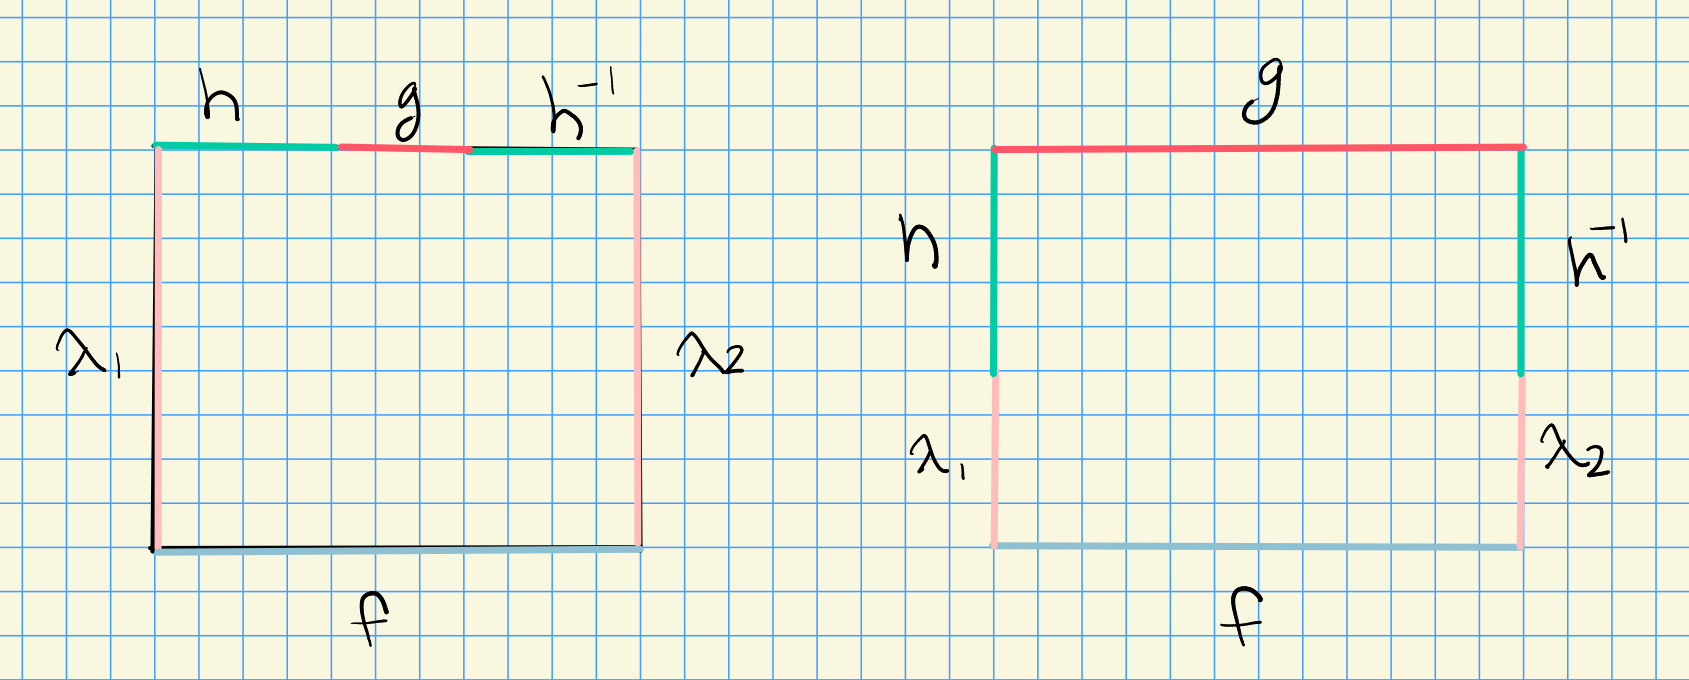
\includegraphics{figures/image_2021-06-04-00-44-45.png}
\caption{image\_2021-06-04-00-44-45}
\end{figure}

\end{solution}

\hypertarget{spring-09spring-07fall-07fall-06-work}{%
\subsection{\texorpdfstring{2 (Spring '09/Spring '07/Fall '07/Fall '06)
\(\work\)}{2 (Spring '09/Spring '07/Fall '07/Fall '06) \textbackslash work}}\label{spring-09spring-07fall-07fall-06-work}}

\begin{enumerate}
\def\labelenumi{\alph{enumi}.}
\item
  State van Kampen's theorem.
\item
  Calculate the fundamental group of the space obtained by taking two
  copies of the torus \(T = S^1 \times S^1\) and gluing them along a
  circle \(S^1 \times {p}\) where \(p\) is a point in \(S^1\).
\item
  Calculate the fundamental group of the Klein bottle.
\item
  Calculate the fundamental group of the one-point union of
  \(S^1 \times S^1\) and \(S^1\).
\item
  Calculate the fundamental group of the one-point union of
  \(S^1 \times S^1\) and \({\mathbb{RP}}^2\).
\end{enumerate}

\begin{quote}
\textbf{Note: multiple appearances!!}
\end{quote}

\hypertarget{fall-18-work-2}{%
\subsection{\texorpdfstring{3 (Fall '18)
\(\work\)}{3 (Fall '18) \textbackslash work}}\label{fall-18-work-2}}

Prove the following portion of van Kampen's theorem. If \(X = A\cup B\)
and \(A\), \(B\), and \(A \cap B\) are nonempty and path connected with
\({\operatorname{pt}}\in A \cap B\), then there is a surjection
\begin{align*}
\pi_1 (A, {\operatorname{pt}}) \ast \pi_1 (B, {\operatorname{pt}}) \to \pi_1 (X, {\operatorname{pt}})
.\end{align*}

\hypertarget{spring-15-work-1}{%
\subsection{\texorpdfstring{4 (Spring '15)
\(\work\)}{4 (Spring '15) \textbackslash work}}\label{spring-15-work-1}}

Let \(X\) denote the quotient space formed from the sphere \(S^2\) by
identifying two distinct points.

Compute the fundamental group and the homology groups of \(X\).

\hypertarget{spring-06-work-2}{%
\subsection{\texorpdfstring{5 (Spring '06)
\(\work\)}{5 (Spring '06) \textbackslash work}}\label{spring-06-work-2}}

Start with the unit disk \({\mathbb{D}}^2\) and identify points on the
boundary if their angles, thought of in polar coordinates, differ a
multiple of \(\pi/2\).

Let \(X\) be the resulting space. Use van Kampen's theorem to compute
\(\pi_1 (X, \ast)\).

\hypertarget{spring-08-work}{%
\subsection{\texorpdfstring{6 (Spring '08)
\(\work\)}{6 (Spring '08) \textbackslash work}}\label{spring-08-work}}

Let \(L\) be the union of the \(z\)-axis and the unit circle in the
\(xy{\hbox{-}}\)plane. Compute
\(\pi_1 ({\mathbb{R}}^3 \backslash L, \ast)\).

\hypertarget{fall-16-work-2}{%
\subsection{\texorpdfstring{7 (Fall '16)
\(\work\)}{7 (Fall '16) \textbackslash work}}\label{fall-16-work-2}}

Let \(A\) be the union of the unit sphere in \({\mathbb{R}}^3\) and the
interval
\(\left\{{(t, 0, 0) : -1 \leq t \leq 1}\right\} \subset {\mathbb{R}}^3\).

Compute \(\pi_1 (A)\) and give an explicit description of the universal
cover of \(X\).

\hypertarget{spring-13-work-1}{%
\subsection{\texorpdfstring{8 (Spring '13)
\(\work\)}{8 (Spring '13) \textbackslash work}}\label{spring-13-work-1}}

\begin{enumerate}
\def\labelenumi{\alph{enumi}.}
\item
  Let \(S_1\) and \(S_2\) be disjoint surfaces. Give the definition of
  their connected sum \(S^1 \#S^2\).
\item
  Compute the fundamental group of the connected sum of the projective
  plane and the two-torus.
\end{enumerate}

\hypertarget{fall-15-work}{%
\subsection{\texorpdfstring{9 (Fall '15)
\(\work\)}{9 (Fall '15) \textbackslash work}}\label{fall-15-work}}

Compute the fundamental group, using any technique you like, of
\({\mathbb{RP}}^2 \#{\mathbb{RP}}^2 \#{\mathbb{RP}}^2\).

\hypertarget{fall-11-work}{%
\subsection{\texorpdfstring{10 (Fall '11)
\(\work\)}{10 (Fall '11) \textbackslash work}}\label{fall-11-work}}

Let
\begin{align*}
V = {\mathbb{D}}^2 \times S^1 = \left\{{ (z, e^{it}) {~\mathrel{\Big|}~}{\left\lVert {z} \right\rVert} \leq 1,~~ 0 \leq t < 2\pi}\right\}
\end{align*}
be the ``solid torus'' with boundary given by the torus
\(T = S^1 \times S^1\) .

For \(n \in {\mathbb{Z}}\) define
\begin{align*} \phi_n : T &\to T \\ (e^{is} , e^{it} ) &\mapsto (e^{is} , e^{i(ns+t)}) .\end{align*}

Find the fundamental group of the identification space
\begin{align*}
V_n = {V{\textstyle\coprod}V \over \sim n}
\end{align*}
where the equivalence relation \(\sim_n\) identifies a point \(x\) on
the boundary \(T\) of the first copy of \(V\) with the point
\(\phi_n (x)\) on the boundary of the second copy of \(V\).

\hypertarget{fall-16-work-3}{%
\subsection{\texorpdfstring{11 (Fall '16)
\(\work\)}{11 (Fall '16) \textbackslash work}}\label{fall-16-work-3}}

Let \(S_k\) be the space obtained by removing \(k\) disjoint open disks
from the sphere \(S^2\). Form \(X_k\) by gluing \(k\) Möbius bands onto
\(S_k\) , one for each circle boundary component of \(S_k\) (by
identifying the boundary circle of a Möbius band homeomorphically with a
given boundary component circle).

Use van Kampen's theorem to calculate \(\pi_1 (X_k)\) for each \(k > 0\)
and identify \(X_k\) in terms of the classification of surfaces.

\hypertarget{spring-13-work-2}{%
\subsection{\texorpdfstring{12 (Spring '13)
\(\work\)}{12 (Spring '13) \textbackslash work}}\label{spring-13-work-2}}

\begin{enumerate}
\def\labelenumi{\alph{enumi}.}
\item
  Let \(A\) be a subspace of a topological space \(X\). Define what it
  means for \(A\) to be a \textbf{deformation retract} of \(X\).
\item
  Consider \(X_1\) the ``planar figure eight'' and
  \begin{align*}X_2 = S^1 \cup ({0} \times [-1, 1])\end{align*}
  (the ``theta space''). Show that \(X_1\) and \(X_2\) have isomorphic
  fundamental groups.
\item
  Prove that the fundamental group of \(X_2\) is a free group on two
  generators.
\end{enumerate}

\hypertarget{spring-2021-4}{%
\subsection{Spring 2021 \#4}\label{spring-2021-4}}

\begin{problem}[Spring 2021, 4]

Suppose that \(X\) is a topological space and \(x_0\in X\), and suppose
that every continuous map \(\gamma: S^1 \to X\) is freely homotopic to
the constant map to \(x_0\). Prove that
\(\pi_1(X, x_0) = \left\{{ e }\right\}\).

\begin{quote}
Note that ``freely'' means there are no conditions on basepoints.
\end{quote}

\end{problem}

\hypertarget{covering-spaces}{%
\section{Covering Spaces}\label{covering-spaces}}

\hypertarget{spring-11spring-14-done}{%
\subsection{\texorpdfstring{1 (Spring 11/Spring '14)
\(\done\)}{1 (Spring 11/Spring '14) \textbackslash done}}\label{spring-11spring-14-done}}

\begin{enumerate}
\def\labelenumi{\alph{enumi}.}
\item
  Give the definition of a \textbf{covering space} \(\widehat{X}\) (and
  \textbf{covering map} \(p : \widehat{X} \to X\)) for a topological
  space \(X\).
\item
  State the homotopy lifting property of covering spaces. Use it to show
  that a covering map \(p : \widehat{X} \to X\) induces an injection
  \begin{align*}
  p^\ast : \pi_1 (\widehat{X}, \widehat{x}) \to \pi_1 (X, p(\widehat{x}))
  \end{align*}
  on fundamental groups.
\item
  Let \(p : \widehat{X} \to X\) be a covering map with \(Y\) and \(X\)
  path-connected. Suppose that the induced map \(p^\ast\) on \(\pi_1\)
  is an isomorphism.
\end{enumerate}

Prove that \(p\) is a homeomorphism.

\todo[inline]{Not done?}

\begin{solution}

\hfill

\begin{concept}

\hfill

\end{concept}

\begin{enumerate}
\def\labelenumi{\alph{enumi}.}
\item
  \todo[inline]{Todo}.
\item
\end{enumerate}

Homotopy lifting property:

\begin{center}
\begin{tikzcd}
                                                                   &  & \tilde X \arrow[dd, "\pi"] \\
                                                                   &  &                            \\
Y\times I \arrow[rr, "H"] \arrow[rruu, "\exists \tilde H", dashed] &  & X                         
\end{tikzcd}
\end{center}

\(\pi\) clearly induces a map \(p_*\) on \(\pi_1\) by functoriality, so
we'll show that \(\ker p_*\) is trivial. Let
\(\gamma: S^1 \to \tilde X \in \pi_1(\tilde X)\) and suppose
\(\alpha \coloneqq p_*(\gamma) = [e] \in \pi_1(X)\). We'll show
\(\gamma \simeq[e]\) in \(\pi_1(\tilde X)\).

Since \(\alpha = [e]\), \(\alpha \simeq{\operatorname{const.}}\) and
thus there is a homotopy \(H: I\times S^1 \to X\) such that
\(H_0 = {\operatorname{const.}}(x_0)\) and \(H_1 = \gamma\). By the HLP,
this lifts to \(\tilde H: I\times S^1 \to \tilde X\). Noting that
\(\pi^{-1}({\operatorname{const.}}(x_0))\) is still a constant loop,
this says that \(\gamma\) is homotopic to a constant loop and thus
nullhomotopic.

\begin{enumerate}
\def\labelenumi{\alph{enumi}.}
\setcounter{enumi}{2}
\tightlist
\item
\end{enumerate}

Since both spaces are path-connected, the degree o the covering map
\(\pi\) is precisely the index of the included fundamental group. This
forces \(\pi\) to be a degree 1 covering and hence a homeomorphism.

\end{solution}

\hypertarget{fall-06fall-09fall-15-work}{%
\subsection{\texorpdfstring{2 (Fall '06/Fall '09/Fall '15)
\(\work\)}{2 (Fall '06/Fall '09/Fall '15) \textbackslash work}}\label{fall-06fall-09fall-15-work}}

\begin{enumerate}
\def\labelenumi{\alph{enumi}.}
\item
  Give the definitions of \textbf{covering space} and \textbf{deck
  transformation} (or covering transformation).
\item
  Describe the universal cover of the Klein bottle and its group of deck
  transformations.
\item
  Explicitly give a collection of deck transformations on
  \begin{align*}\left\{{(x, y) \mathrel{\Big|}-1 \leq x \leq 1, -\infty < y < \infty}\right\}\end{align*}
  such that the quotient is a Möbius band.
\item
  Find the universal cover of \({\mathbb{RP}}^2 \times S^1\) and
  explicitly describe its group of deck transformations.
\end{enumerate}

\hypertarget{spring-2021-5}{%
\subsection{Spring 2021 \#5}\label{spring-2021-5}}

\begin{problem}[Spring 2021, 5]

Identify five mutually non-homeomorphic connected spaces \(X\) for which
there is a covering map \(p:X\to K\) where \(K\) is the Klein bottle.
Give an example of the covering in each case.

\end{problem}

\hypertarget{spring-06spring-07spring-12-work}{%
\subsection{\texorpdfstring{3 (Spring '06/Spring '07/Spring '12)
\(\work\)}{3 (Spring '06/Spring '07/Spring '12) \textbackslash work}}\label{spring-06spring-07spring-12-work}}

\begin{enumerate}
\def\labelenumi{\alph{enumi}.}
\item
  What is the definition of a \textbf{regular} (or Galois) covering
  space?
\item
  State, without proof, a criterion in terms of the fundamental group
  for a covering map \(p : \tilde X \to X\) to be regular.
\item
  Let \(\Theta\) be the topological space formed as the union of a
  circle and its diameter (so this space looks exactly like the letter
  \(\Theta\)). Give an example of a covering space of \(\Theta\) that is
  not regular.
\end{enumerate}

\hypertarget{spring-08-work-1}{%
\subsection{\texorpdfstring{4 (Spring '08)
\(\work\)}{4 (Spring '08) \textbackslash work}}\label{spring-08-work-1}}

Let \(S\) be the closed orientable surface of genus 2 and let \(C\) be
the commutator subgroup of \(\pi_1 (S, \ast)\). Let \(\tilde S\) be the
cover corresponding to \(C\). Is the covering map \(\tilde S \to S\)
regular?

\begin{quote}
The term ``normal'' is sometimes used as a synonym for regular in this
context.
\end{quote}

What is the group of deck transformations?

Give an example of a nontrivial element of \(\pi_1 (S, \ast)\) which
lifts to a trivial deck transformation.

\hypertarget{fall-04-work-2}{%
\subsection{\texorpdfstring{5 (Fall '04)
\(\work\)}{5 (Fall '04) \textbackslash work}}\label{fall-04-work-2}}

Describe the 3-fold connected covering spaces of \(S^1 \lor S^1\).

\hypertarget{spring-17-done}{%
\subsection{\texorpdfstring{6 (Spring '17)
\(\done\)}{6 (Spring '17) \textbackslash done}}\label{spring-17-done}}

Find all three-fold covers of the wedge of two copies of
\({\mathbb{RP}}^2\) . Justify your answer.

\begin{solution}

\hfill

\begin{concept}

\hfill

\end{concept}

Note \(\pi_1 {\mathbb{RP}}^2 = {\mathbb{Z}}/2{\mathbb{Z}}\), so
\(\pi_1 X = ({\mathbb{Z}}/2{\mathbb{Z}})^2\).

The pullback of any neighborhood of the basepoint needs to be locally
homeomorphic to one of

\begin{itemize}
\tightlist
\item
  \(S^2 \vee S^2\)
\item
  \({\mathbb{RP}}^2 \vee S^2\)
\end{itemize}

And so \emph{all} possibilities for regular covering spaces are given by

\begin{itemize}
\tightlist
\item
  \(\bigvee^{2k} S^2\) ``beads'' wrapped into a necklace for any
  \(k \geq 1\)
\item
  \({\mathbb{RP}}^2 \vee (\bigvee^k S^2) \vee {\mathbb{RP}}^2\)
\item
  \(\vee^\infty S^2\), the universal cover
\end{itemize}

To get a threefold cover, we want the basepoint to lift to three
preimages, so we can take

\begin{itemize}
\tightlist
\item
  \(S^2 \vee S^2 \vee S^2\) wrapped
\item
  \({\mathbb{RP}}^2 \vee S^2 \vee {\mathbb{RP}}^2\).
\end{itemize}

\end{solution}

\hypertarget{fall-17-done}{%
\subsection{\texorpdfstring{7 (Fall '17)
\(\done\)}{7 (Fall '17) \textbackslash done}}\label{fall-17-done}}

Describe, as explicitly as you can, two different (non-homeomorphic)
connected two-sheeted covering spaces of
\({\mathbb{RP}}^2 \lor {\mathbb{RP}}^3\), and prove that they are not
homeomorphic.

\todo[inline]{Expand solution.}

\begin{solution}

\hfill

\begin{concept}

\hfill

\end{concept}

\begin{itemize}
\tightlist
\item
  \({\mathbb{RP}}_3 \vee S^2 \vee {\mathbb{RP}}^3\), which has
  \(\pi_2 = 0 \ast {\mathbb{Z}}\ast 0 = {\mathbb{Z}}\) since
  \(\pi_{i\geq 1} X = \pi_{i\geq 1}\tilde X\) and
  \(\tilde {\mathbb{RP}}^3 = S^3\).
\item
  \({\mathbb{RP}}^2 \vee S^3 \vee {\mathbb{RP}}^2\), which has
  \(\pi_2 = {\mathbb{Z}}\ast 0 \ast {\mathbb{Z}}= {\mathbb{Z}}\ast {\mathbb{Z}}\neq {\mathbb{Z}}\)
\end{itemize}

\end{solution}

\hypertarget{spring-19-done}{%
\subsection{\texorpdfstring{8 (Spring '19)
\(\done\)}{8 (Spring '19) \textbackslash done}}\label{spring-19-done}}

Is there a covering map from
\begin{align*}
X_3 = \left\{{x^2 + y^2 = 1}\right\} \cup \left\{{(x - 2)^2 + y^2 = 1}\right\} \cup \left\{{(x + 2)^2 + y^2 = 1}\right\} \subset {\mathbb{R}}^2
\end{align*}
to \(S^1 \vee S^1\)? If there is, give an example; if not, give a proof.

\begin{solution}

\hfill

\begin{concept}

\hfill

\end{concept}

Yes,

\begin{figure}
\centering
\includegraphics{figures/2020-02-04-21:50.png}
\caption{Image}
\end{figure}

\end{solution}

\hypertarget{spring-05-work}{%
\subsection{\texorpdfstring{9 (Spring '05)
\(\work\)}{9 (Spring '05) \textbackslash work}}\label{spring-05-work}}

\begin{enumerate}
\def\labelenumi{\alph{enumi}.}
\item
  Suppose \(Y\) is an \(n\)-fold connected covering space of the torus
  \(S^1 \times S^1\). Up to homeomorphism, what is \(Y\)? Justify your
  answer.
\item
  Let \(X\) be the topological space obtained by deleting a disk from a
  torus. Suppose \(Y\) is a 3-fold covering space of \(X\).

  What surfaces could \(Y\) be? Justify your answer, but you need not
  exhibit the covering maps explicitly.
\end{enumerate}

\hypertarget{spring-07-work}{%
\subsection{\texorpdfstring{10 (Spring '07)
\(\work\)}{10 (Spring '07) \textbackslash work}}\label{spring-07-work}}

Let \(S\) be a connected surface, and let \(U\) be a connected open
subset of \(S\). Let \(p : \tilde S \to S\) be the universal cover of
\(S\). Show that \(p^{-1}(U )\) is connected if and only if the
homeomorphism \(i_\ast : \pi_1 (U ) \to \pi_1 (S)\) induced by the
inclusion \(i : U \to S\) is onto.

\hypertarget{fall-10-work}{%
\subsection{\texorpdfstring{11 (Fall '10)
\(\work\)}{11 (Fall '10) \textbackslash work}}\label{fall-10-work}}

Suppose that X has universal cover \(p : \tilde X \to X\) and let
\(A \subset X\) be a subspace with \(p(\tilde a) = a \in A\). Show that
there is a group isomorphism
\begin{align*}
\ker(\pi_1 (A, a) \to \pi_1 (X, a)) \cong \pi_1 (p^{-1}A, \mkern 1.5mu\overline{\mkern-1.5mua\mkern-1.5mu}\mkern 1.5mu)
.\end{align*}

\hypertarget{fall-14-work-2}{%
\subsection{\texorpdfstring{12 (Fall '14)
\(\work\)}{12 (Fall '14) \textbackslash work}}\label{fall-14-work-2}}

Prove that every continuous map \(f : {\mathbb{RP}}^2 \to S^1\) is
homotopic to a constant.

\begin{quote}
Hint: think about covering spaces.
\end{quote}

\hypertarget{spring-16-work-1}{%
\subsection{\texorpdfstring{13 (Spring '16)
\(\work\)}{13 (Spring '16) \textbackslash work}}\label{spring-16-work-1}}

Prove that the free group on two generators contains a subgroup
isomorphic to the free group on five generators by constructing an
appropriate covering space of \(S^1 \lor S^1\).

\hypertarget{fall-12-work-1}{%
\subsection{\texorpdfstring{14 (Fall '12)
\(\work\)}{14 (Fall '12) \textbackslash work}}\label{fall-12-work-1}}

Use covering space theory to show that
\({\mathbb{Z}}_2 \ast {\mathbb{Z}}\) (that is, the free product of
\({\mathbb{Z}}_2\) and \({\mathbb{Z}}\)) has two subgroups of index 2
which are not isomorphic to each other.

\hypertarget{spring-17-work}{%
\subsection{\texorpdfstring{15 (Spring '17)
\(\work\)}{15 (Spring '17) \textbackslash work}}\label{spring-17-work}}

\begin{enumerate}
\def\labelenumi{\alph{enumi}.}
\item
  Show that any finite index subgroup of a finitely generated free group
  is free. State clearly any facts you use about the fundamental groups
  of graphs.
\item
  Prove that if \(N\) is a nontrivial normal subgroup of infinite index
  in a finitely generated free group \(F\) , then \(N\) is not finitely
  generated.
\end{enumerate}

\hypertarget{spring-19-work}{%
\subsection{\texorpdfstring{16 (Spring '19)
\(\work\)}{16 (Spring '19) \textbackslash work}}\label{spring-19-work}}

Let \(p : X \to Y\) be a covering space, where \(X\) is compact,
path-connected, and locally path-connected.

Prove that for each \(x \in X\) the set
\(p^{-1}(\left\{{p(x)}\right\})\) is finite, and has cardinality equal
to the index of \(p_* (\pi_1 (X, x))\) in \(\pi_1 (Y, p(x))\).

\hypertarget{cell-complexes-and-adjunction-spaces}{%
\section{Cell Complexes and Adjunction
Spaces}\label{cell-complexes-and-adjunction-spaces}}

\hypertarget{fall-07-work-1}{%
\subsection{\texorpdfstring{1 (Fall '07)
\(\work\)}{1 (Fall '07) \textbackslash work}}\label{fall-07-work-1}}

Describe a cell complex structure on the torus \(T = S^1 \times S^1\)
and use this to compute the homology groups of \(T\).

\begin{quote}
To justify your answer you will need to consider the attaching maps in
detail.
\end{quote}

\hypertarget{fall-04-work-3}{%
\subsection{\texorpdfstring{2 (Fall '04)
\(\work\)}{2 (Fall '04) \textbackslash work}}\label{fall-04-work-3}}

Let \(X\) be the space formed by identifying the boundary of a Möbius
band with a meridian of the torus \(T^2\).

Compute \(\pi_1 (X)\) and \(H_* (X)\).

\hypertarget{spring-06-work-3}{%
\subsection{\texorpdfstring{3 (Spring '06)
\(\work\)}{3 (Spring '06) \textbackslash work}}\label{spring-06-work-3}}

Compute the homology of the space \(X\) obtained by attaching a Möbius
band to \({\mathbb{RP}}^2\) via a homeomorphism of its boundary circle
to the standard \({\mathbb{RP}}^1\) in \({\mathbb{RP}}^2\).

\hypertarget{spring-14-work}{%
\subsection{\texorpdfstring{4 (Spring '14)
\(\work\)}{4 (Spring '14) \textbackslash work}}\label{spring-14-work}}

Let \(X\) be a space obtained by attaching two 2-cells to the torus
\(S^1 \times S^1\), one along a simple closed curve
\(\left\{{x}\right\} \times S^1\) and the other along
\(\left\{{y}\right\} \times S^1\) for two points \(x \neq y\) in \(S^1\)
.

\hypertarget{a}{%
\subsubsection{a}\label{a}}

Draw an embedding of \(X\) in \({\mathbb{R}}^3\) and calculate its
fundamental group.

\hypertarget{b}{%
\subsubsection{b}\label{b}}

Calculate the homology groups of \(X\).

\hypertarget{fall-07-work-2}{%
\subsection{\texorpdfstring{5 (Fall '07)
\(\work\)}{5 (Fall '07) \textbackslash work}}\label{fall-07-work-2}}

Let \(X\) be the space obtained as the quotient of a disjoint union of a
2-sphere \(S^2\) and a torus \(T = S^1 \times S^1\) by identifying the
equator in \(S^2\) with a circle \(S^1 \times \left\{{p}\right\}\) in
\(T\).

Compute the homology groups of \(X\).

\hypertarget{spring-06-work-4}{%
\subsection{\texorpdfstring{6 (Spring '06)
\(\work\)}{6 (Spring '06) \textbackslash work}}\label{spring-06-work-4}}

Let \(X = S^2 / \left\{{p_1 = \cdots = p_k }\right\}\) be the
topological space obtained from the 2-sphere by identifying \(k\)
distinct points on it (\(k \geq 2\)).

Find:

\begin{enumerate}
\def\labelenumi{\alph{enumi}.}
\item
  The fundamental group of \(X\).
\item
  The Euler characteristic of \(X\).
\item
  The homology groups of \(X\).
\end{enumerate}

\hypertarget{fall-16-work-4}{%
\subsection{\texorpdfstring{7 (Fall '16)
\(\work\)}{7 (Fall '16) \textbackslash work}}\label{fall-16-work-4}}

Let \(X\) be the topological space obtained as the quotient of the
sphere
\(S^2 = \left\{{\mathbf{x} \in {\mathbb{R}}^3 {~\mathrel{\Big|}~}{\left\lVert {\mathbf{x}} \right\rVert} = 1}\right\}\)
under the equivalence relation \(\mathbf{x} \sim -\mathbf{x}\) for
\(\mathbf{x}\) in the equatorial circle, i.e.~for
\(\mathbf{x} = (x_1, x_2, 0)\).

Calculate \(H_* (X; {\mathbb{Z}})\) from a CW complex description of
\(X\).

\hypertarget{fall-17-work-2}{%
\subsection{\texorpdfstring{8 (Fall '17)
\(\work\)}{8 (Fall '17) \textbackslash work}}\label{fall-17-work-2}}

Compute, by any means available, the fundamental group and all the
homology groups of the space obtained by gluing one copy \(A\) of
\(S^2\) to another copy \(B\) of \(S^2\) via a two-sheeted covering
space map from the equator of \(A\) onto the equator of \(B\).

\hypertarget{spring-14-work-1}{%
\subsection{\texorpdfstring{9 (Spring '14)
\(\work\)}{9 (Spring '14) \textbackslash work}}\label{spring-14-work-1}}

Use cellular homology to calculate the homology groups of
\(S^n \times S^m\).

\hypertarget{fall-09fall-12-work}{%
\subsection{\texorpdfstring{10 (Fall '09/Fall '12)
\(\work\)}{10 (Fall '09/Fall '12) \textbackslash work}}\label{fall-09fall-12-work}}

Denote the points of \(S^1 \times I\) by \((z, t)\) where \(z\) is a
unit complex number and \(0 \leq t \leq 1\). Let \(X\) denote the
quotient of \(S^1 \times I\) given by identifying \((z, 1)\) and
\((z_2 , 0)\) for all \(z \in S^1\).

Give a cell structure, with attaching maps, for \(X\), and use it to
compute \(\pi_1 (X, \ast)\) and \(H_1 (X)\).

\hypertarget{spring-15-work-2}{%
\subsection{\texorpdfstring{11 (Spring '15)
\(\work\)}{11 (Spring '15) \textbackslash work}}\label{spring-15-work-2}}

Let \(X = S_1 \cup S_2 \subset {\mathbb{R}}^3\) be the union of two
spheres of radius 2, one about \((1, 0, 0)\) and the other about
\((-1, 0, 0)\), i.e.~
\begin{align*}  
S_1 &= \left\{{(x, y,z) \mathrel{\Big|}(x-1)^2 + y^2 +z^2 = 4}\right\} \\
S_2 &= \left\{{(x, y, z) \mathrel{\Big|}(x + 1)^2 + y^2 + z^2 = 4}\right\}
.\end{align*}

\begin{enumerate}
\def\labelenumi{\alph{enumi}.}
\item
  Give a description of \(X\) as a CW complex.
\item
  Write out the cellular chain complex of \(X\).
\item
  Calculate \(H_* (X; Z)\).
\end{enumerate}

\hypertarget{spring-06-work-5}{%
\subsection{\texorpdfstring{12 (Spring '06)
\(\work\)}{12 (Spring '06) \textbackslash work}}\label{spring-06-work-5}}

Let \(M\) and \(N\) be finite CW complexes.

\begin{enumerate}
\def\labelenumi{\alph{enumi}.}
\item
  Describe a cellular structure of \(M \times N\) in terms of the
  cellular structures of \(M\) and \(N\).
\item
  Show that the Euler characteristic of \(M \times N\) is the product of
  the Euler characteristics of \(M\) and \(N\).
\end{enumerate}

\hypertarget{spring-07-work-1}{%
\subsection{\texorpdfstring{13 (Spring '07)
\(\work\)}{13 (Spring '07) \textbackslash work}}\label{spring-07-work-1}}

Suppose the space \(X\) is obtained by attaching a 2-cell to the torus
\(S^1 \times S^1\).

In other words, \(X\) is the quotient space of the disjoint union of the
closed disc \({\mathbb{D}}^2\) and the torus \(S^1 \times S^1\) by the
identification \(x \sim f(x)\) where \(S^1\) is the boundary of the unit
disc and \(f : S^1 \to S^1 \times S^1\) is a continuous map.

What are the possible homology groups of \(X\)? Justify your answer.

\hypertarget{spring-15-work-3}{%
\subsection{\texorpdfstring{14 (Spring '15)
\(\work\)}{14 (Spring '15) \textbackslash work}}\label{spring-15-work-3}}

Let \(X\) be the topological space constructed by attaching a closed
2-disk \({\mathbb{D}}^2\) to the circle \(S^1\) by a continuous map
\(\partial{\mathbb{D}}^2 \to S^1\) of degree \(d > 0\) on the boundary
circle.

\begin{enumerate}
\def\labelenumi{\alph{enumi}.}
\item
  Show that every continuous map \(X \to X\) has a fixed point.
\item
  Explain how to obtain all the connected covering spaces of \(X\).
\end{enumerate}

\hypertarget{spring-11-work-2}{%
\subsection{\texorpdfstring{15 (Spring '11)
\(\work\)}{15 (Spring '11) \textbackslash work}}\label{spring-11-work-2}}

Let \(X\) be a topological space obtained by attaching a 2-cell to
\({\mathbb{RP}}^2\) via some map \(f: S^1 \to {\mathbb{RP}}^2\) .

What are the possibilities for the homology \(H_* (X; Z)\)?

\hypertarget{spring-12-work-1}{%
\subsection{\texorpdfstring{16 (Spring '12)
\(\work\)}{16 (Spring '12) \textbackslash work}}\label{spring-12-work-1}}

For any integer \(n \geq 2\) let \(X_n\) denote the space formed by
attaching a 2-cell to the circle \(S^1\) via the attaching map
\begin{align*}  
a_n: S^1 &\to S^1 \\
e^{i\theta} &\mapsto e^{in\theta}
.\end{align*}

\hypertarget{a-1}{%
\subsubsection{a}\label{a-1}}

Compute the fundamental group and the homology of \(X_n\).

\hypertarget{b-1}{%
\subsubsection{b}\label{b-1}}

Exactly one of the \(X_n\) (for \(n \geq 2\)) is homeomorphic to a
surface. Identify, with proof, both this value of \(n\) and the surface
that \(X_n\) is homeomorphic to (including a description of the
homeomorphism).

\hypertarget{spring-09-work-2}{%
\subsection{\texorpdfstring{17 (Spring '09)
\(\work\)}{17 (Spring '09) \textbackslash work}}\label{spring-09-work-2}}

Let \(X\) be a CW complex and let \(\pi : Y \to X\) be a covering space.

\hypertarget{a-2}{%
\subsubsection{a}\label{a-2}}

Show that \(Y\) is compact iff \(X\) is compact and \(\pi\) has finite
degree.

\hypertarget{b-2}{%
\subsubsection{b}\label{b-2}}

Assume that \(\pi\) has finite degree \(d\). Show show that
\(\chi (Y ) = d \chi (X)\).

\hypertarget{c}{%
\subsubsection{c}\label{c}}

Let \(\pi :{\mathbb{RP}}^N \to X\) be a covering map. Show that if \(N\)
is even, \(\pi\) is a homeomorphism.

\hypertarget{spring-18-work-1}{%
\subsection{\texorpdfstring{18 (Spring '18)
\(\work\)}{18 (Spring '18) \textbackslash work}}\label{spring-18-work-1}}

For topological spaces \(X, Y\) the \textbf{mapping cone} \(C(f )\) of a
map \(f : X \to Y\) is defined to be the quotient space
\begin{align*}  
(X \times [0, 1]){\textstyle\coprod}Y / \sim &{\quad \operatorname{where} \quad}  \\ 
(x, 0) &\sim (x', 0) {\quad \operatorname{for all} \quad} x, x' \in X \text{ and } \\ 
(x, 1) &\sim f (x) {\quad \operatorname{for all } \quad} x \in X
.\end{align*}

Let \(\phi_k : S^n \to S^n\) be a degree \(k\) map for some integer
\(k\).

Find \(H_i(C(\phi_k ))\) for all \(i\).

\hypertarget{spring-2019-7-done}{%
\subsection{\texorpdfstring{Spring 2019 \#7
\(\done\)}{Spring 2019 \#7 \textbackslash done}}\label{spring-2019-7-done}}

For \(f:X\to Y\), the \emph{mapping cone} of \(f\) is defined as
\begin{align*}  
C_f \coloneqq\qty{X\times I} {\textstyle\coprod}Y/\sim \\
(x, 0) \sim (x', 0) \quad \text{for all }x, x'\in X\\
(x, 1) \sim f(x)
.\end{align*}

Let \(\phi_k: S^1\to S^1\) be a \(k{\hbox{-}}\)fold covering and find
\(\pi_1\qty{C_f}\).

\todo[inline]{Revisit, old. Maybe redo.}

\begin{solution}

\hfill

\begin{concept}

\hfill

\end{concept}

Let \(f: S^1 \xrightarrow{\times k} S^1\).

\textbf{Claim:} The inclusion \(S^1 \to C_\phi\) induces an isomorphism
\(\pi_1(C_\phi) \cong \pi_1(S^1) / H\) where
\(H = N_{\pi_1(S^1)}(\left\langle{f^*}\right\rangle)\) is the normal
subgroup generated by the induced map \(f^* \pi_1(S^1) \to \pi_1(S^1)\).

\begin{itemize}
\item
  Since \(f\) is a \(k{\hbox{-}}\)fold cover, the induced map is
  multiplication by \(k\) on the generator \(\alpha \in \pi_1(S^1)\),
  i.e.~\(\alpha \mapsto \alpha^k\).
\item
  But then \(\pi_1(S^1) \cong {\mathbb{Z}}\) and
  \(H \cong k{\mathbb{Z}}\), so
  \(\pi_1(C_\phi) \cong {\mathbb{Z}}/m{\mathbb{Z}}\).
\end{itemize}

\end{solution}

\hypertarget{fall-18-work-3}{%
\subsection{\texorpdfstring{19 (Fall '18)
\(\work\)}{19 (Fall '18) \textbackslash work}}\label{fall-18-work-3}}

Prove that a finite CW complex must be Hausdorff.

\hypertarget{homology-and-degree-theory}{%
\section{Homology and Degree Theory}\label{homology-and-degree-theory}}

\hypertarget{spring-09-work-3}{%
\subsection{\texorpdfstring{1 (Spring '09)
\(\work\)}{1 (Spring '09) \textbackslash work}}\label{spring-09-work-3}}

Compute the homology of the one-point union of \(S^1 \times S^1\) and
\(S^1\).

\hypertarget{fall-06-work-1}{%
\subsection{\texorpdfstring{2 (Fall '06)
\(\work\)}{2 (Fall '06) \textbackslash work}}\label{fall-06-work-1}}

\begin{enumerate}
\def\labelenumi{\alph{enumi}.}
\item
  State the \textbf{Mayer-Vietoris theorem}.
\item
  Use it to compute the homology of the space \(X\) obtained by gluing
  two solid tori along their boundary as follows. Let \({\mathbb{D}}^2\)
  be the unit disk and let \(S^1\) be the unit circle in the complex
  plane \({\mathbb{C}}\). Let \(A = S^1 \times {\mathbb{D}}^2\) and
  \(B = {\mathbb{D}}^2 \times S^1\).
\end{enumerate}

Then \(X\) is the quotient space of the disjoint union
\(A {\textstyle\coprod}B\) obtained by identifying \((z, w) \in A\) with
\((zw^3 , w) \in B\) for all \((z, w) \in S^1 \times S^1\).

\hypertarget{fall-12-work-2}{%
\subsection{\texorpdfstring{3 (Fall '12)
\(\work\)}{3 (Fall '12) \textbackslash work}}\label{fall-12-work-2}}

Let \(A\) and \(B\) be circles bounding disjoint disks in the plane
\(z = 0\) in \({\mathbb{R}}^3\). Let \(X\) be the subset of the upper
half-space of \({\mathbb{R}}^3\) that is the union of the plane
\(z = 0\) and a (topological) cylinder that intersects the plane in
\(\partial C = A \cup B\).

Compute \(H_* (X)\) using the Mayer--Vietoris sequence.

\hypertarget{fall-14-work-3}{%
\subsection{\texorpdfstring{4 (Fall '14)
\(\work\)}{4 (Fall '14) \textbackslash work}}\label{fall-14-work-3}}

Compute the integral homology groups of the space \(X = Y \cup Z\) which
is the union of the sphere
\begin{align*}
Y = \left\{{x^2 + y^2 + z^2 = 1}\right\}
\end{align*}
and the ellipsoid
\begin{align*}
Z =  \left\{{x^2 + y^2 + {z^2 \over 4} = 1}\right\}
.\end{align*}

\hypertarget{spring-08-work-2}{%
\subsection{\texorpdfstring{5 (Spring '08)
\(\work\)}{5 (Spring '08) \textbackslash work}}\label{spring-08-work-2}}

Let \(X\) consist of two copies of the solid torus
\({\mathbb{D}}^2 \times S^1\), glued together by the identity map along
the boundary torus \(S^1 \times S^1\). Compute the homology groups of
\(X\).

\hypertarget{spring-17-work-1}{%
\subsection{\texorpdfstring{6 (Spring '17)
\(\work\)}{6 (Spring '17) \textbackslash work}}\label{spring-17-work-1}}

Use the circle along which the connected sum is performed and the
Mayer-Vietoris long exact sequence to compute the homology of
\({\mathbb{RP}}^2 \# {\mathbb{RP}}^2\).

\hypertarget{fall-15-work-1}{%
\subsection{\texorpdfstring{7 (Fall '15)
\(\work\)}{7 (Fall '15) \textbackslash work}}\label{fall-15-work-1}}

Express a Klein bottle as the union of two annuli.

Use the Mayer Vietoris sequence and this decomposition to compute its
homology.

\hypertarget{spring-09-work-4}{%
\subsection{\texorpdfstring{8 (Spring '09)
\(\work\)}{8 (Spring '09) \textbackslash work}}\label{spring-09-work-4}}

Let \(X\) be the topological space obtained by identifying three
distinct points on \(S^2\). Calculate \(H_* (X; Z)\).

\hypertarget{fall-05-work}{%
\subsection{\texorpdfstring{9 (Fall '05)
\(\work\)}{9 (Fall '05) \textbackslash work}}\label{fall-05-work}}

Compute \(H_0\) and \(H_1\) of the complete graph \(K_5\) formed by
taking five points and joining each pair with an edge.

\hypertarget{fall-18-work-4}{%
\subsection{\texorpdfstring{10 (Fall '18)
\(\work\)}{10 (Fall '18) \textbackslash work}}\label{fall-18-work-4}}

Compute the homology of the subset \(X \subset {\mathbb{R}}^3\) formed
as the union of the unit sphere, the \(z{\hbox{-}}\)axis, and the
\(xy{\hbox{-}}\)plane.

\hypertarget{spring-05fall-13-work}{%
\subsection{\texorpdfstring{11 (Spring '05/Fall '13)
\(\work\)}{11 (Spring '05/Fall '13) \textbackslash work}}\label{spring-05fall-13-work}}

Let \(X\) be the topological space formed by filling in two circles
\(S^1 \times \left\{{p_1 }\right\}\) and
\(S^1 \times \left\{{p_2 }\right\}\) in the torus \(S^1 \times S^1\)
with disks.

Calculate the fundamental group and the homology groups of \(X\).

\hypertarget{spring-19-work-1}{%
\subsection{\texorpdfstring{12 (Spring '19)
\(\work\)}{12 (Spring '19) \textbackslash work}}\label{spring-19-work-1}}

\begin{enumerate}
\def\labelenumi{\alph{enumi}.}
\tightlist
\item
  Consider the quotient space
  \begin{align*}
  T^2 = {\mathbb{R}}^2 / \sim {\quad \operatorname{where} \quad} (x, y) \sim (x + m, y + n) \text{ for } m, n \in {\mathbb{Z}}
  ,\end{align*}
  and let \(A\) be any \(2 \times 2\) matrix whose entries are integers
  such that \(\det A = 1\).
\end{enumerate}

Prove that the action of \(A\) on \({\mathbb{R}}^2\) descends via the
quotient \({\mathbb{R}}^2 \to T^2\) to induce a homeomorphism
\(T^2 \to T^2\).

\begin{enumerate}
\def\labelenumi{\alph{enumi}.}
\setcounter{enumi}{1}
\tightlist
\item
  Using this homeomorphism of \(T^2\), we define a new quotient space
  \begin{align*}
  T_A^3 \coloneqq{T^2\times{\mathbb{R}}\over \sim} {\quad \operatorname{where} \quad} ((x, y), t) \sim (A(x, y), t + 1)
  \end{align*}
\end{enumerate}

Compute \(H_1 (T_A^3 )\) if
\(A=\left(\begin{array}{ll} 1 & 1 \\ 0 & 1 \end{array}\right).\)

\hypertarget{spring-12-work-2}{%
\subsection{\texorpdfstring{13 (Spring '12)
\(\work\)}{13 (Spring '12) \textbackslash work}}\label{spring-12-work-2}}

Give a self-contained proof that the zeroth homology \(H_0 (X)\) is
isomorphic to \({\mathbb{Z}}\) for every path-connected space \(X\).

\hypertarget{fall-18-work-5}{%
\subsection{\texorpdfstring{14 (Fall '18)
\(\work\)}{14 (Fall '18) \textbackslash work}}\label{fall-18-work-5}}

It is a fact that if \(X\) is a single point then
\(H_1 (X) = \left\{{0}\right\}\).

One of the following is the correct justification of this fact in terms
of the singular chain complex.

Which one is correct and why is it correct?

\begin{enumerate}
\def\labelenumi{\alph{enumi}.}
\item
  \(C_1 (X) = \left\{{0}\right\}\).
\item
  \(C_1 (X) \neq \left\{{0}\right\}\) but \(\ker \partial_1 = 0\) with
  \(\partial_1 : C_1 (X) \to C_0 (X)\).
\item
  \(\ker \partial_1 \neq 0\) but
  \(\ker \partial_1 = \operatorname{im}\partial_2\) with
  \(\partial_2 : C_2 (X) \to C_1 (X)\).
\end{enumerate}

\hypertarget{fall-10-work-1}{%
\subsection{\texorpdfstring{15 (Fall '10)
\(\work\)}{15 (Fall '10) \textbackslash work}}\label{fall-10-work-1}}

Compute the homology groups of \(S^2 \times S^2\).

\hypertarget{fall-16-work-5}{%
\subsection{\texorpdfstring{16 (Fall '16)
\(\work\)}{16 (Fall '16) \textbackslash work}}\label{fall-16-work-5}}

Let \(\Sigma\) be a closed orientable surface of genus \(g\). Compute
\(H_i(S^1 \times \Sigma; Z)\) for \(i = 0, 1, 2, 3\).

\hypertarget{spring-07-work-2}{%
\subsection{\texorpdfstring{17 (Spring '07)
\(\work\)}{17 (Spring '07) \textbackslash work}}\label{spring-07-work-2}}

Prove that if \(A\) is a retract of the topological space \(X\), then
for all nonnegative integers \(n\) there is a group \(G_n\) such that
\(H_{n} (X) \cong H_{n} (A) \oplus G_n\).

\begin{quote}
Here \(H_{n}\) denotes the \(n\)th singular homology group with integer
coefficients.
\end{quote}

\hypertarget{spring-13-work-3}{%
\subsection{\texorpdfstring{18 (Spring '13)
\(\work\)}{18 (Spring '13) \textbackslash work}}\label{spring-13-work-3}}

Does there exist a map of degree 2013 from \(S^2 \to S^2\).

\hypertarget{fall-18-work-6}{%
\subsection{\texorpdfstring{19 (Fall '18)
\(\work\)}{19 (Fall '18) \textbackslash work}}\label{fall-18-work-6}}

For each \(n \in {\mathbb{Z}}\) give an example of a map
\(f_n : S^2 \to S^2\).

For which \(n\) must any such map have a fixed point?

\hypertarget{spring-09-work-5}{%
\subsection{\texorpdfstring{20 (Spring '09)
\(\work\)}{20 (Spring '09) \textbackslash work}}\label{spring-09-work-5}}

\begin{enumerate}
\def\labelenumi{\alph{enumi}.}
\tightlist
\item
  What is the degree of the antipodal map on the \(n\)-sphere?
\end{enumerate}

(No justification required)

\begin{enumerate}
\def\labelenumi{\alph{enumi}.}
\setcounter{enumi}{1}
\item
  Define a CW complex homeomorphic to the real projective
  \(n{\hbox{-}}\)space \({\mathbb{RP}}^n\).
\item
  Let \(\pi : {\mathbb{RP}}^n \to X\) be a covering map. Show that if
  \(n\) is even, \(\pi\) is a homeomorphism.
\end{enumerate}

\hypertarget{fall-17-work-3}{%
\subsection{\texorpdfstring{21 (Fall '17)
\(\work\)}{21 (Fall '17) \textbackslash work}}\label{fall-17-work-3}}

Let \(A \subset X\). Prove that the relative homology group
\(H_0 (X, A)\) is trivial if and only if \(A\) intersects every path
component of \(X\).

\hypertarget{fall-18-work-7}{%
\subsection{\texorpdfstring{22 (Fall '18)
\(\work\)}{22 (Fall '18) \textbackslash work}}\label{fall-18-work-7}}

Let \({\mathbb{D}}\) be a closed disk embedded in the torus
\(T = S^1 \times S^1\) and let \(X\) be the result of removing the
interior of \({\mathbb{D}}\) from \(T\) . Let \(B\) be the boundary of
\(X\), i.e.~the circle boundary of the original closed disk
\({\mathbb{D}}\).

Compute \(H_i (T, B)\) for all \(i\).

\hypertarget{fall-11-work-1}{%
\subsection{\texorpdfstring{23 (Fall '11)
\(\work\)}{23 (Fall '11) \textbackslash work}}\label{fall-11-work-1}}

For any \(n \geq 1\) let
\(S^n = \left\{{(x_0 , \cdots , x_n )\mathrel{\Big|}\sum x_i^2 =1}\right\}\)
denote the \(n\) dimensional unit sphere and let
\begin{align*}E = \left\{{(x_0 , . . . , x_n )\mathrel{\Big|}x_n = 0}\right\}\end{align*}
denote the ``equator''.

Find, for all \(k\), the relative homology \(H_k (S^n , E)\).

\hypertarget{spring-12spring-15-work}{%
\subsection{\texorpdfstring{24 (Spring '12/Spring '15)
\(\work\)}{24 (Spring '12/Spring '15) \textbackslash work}}\label{spring-12spring-15-work}}

Suppose that \(U\) and \(V\) are open subsets of a space \(X\), with
\(X = U \cup V\). Find, with proof, a general formula relating the Euler
characteristics of \(X, U, V\), and \(U \cap V\).

\begin{quote}
You may assume that the homologies of \(U, V, U \cap V, X\) are
finite-dimensional so that their Euler characteristics are well defined.
\end{quote}

\hypertarget{spring-2021-6}{%
\subsection{Spring 2021 \#6}\label{spring-2021-6}}

\begin{problem}[Spring 2021, 6]

For each of the following spaces, compute the fundamental group and the
homology groups.

\begin{enumerate}
\def\labelenumi{\alph{enumi}.}
\item
  The graph \(\Theta\) consisting of two edges and three vertices
  connecting them.
\item
  The 2-dimensional cell complex \(\Theta_2\) consisting of a closed
  circle and three 2-dimensional disks each having boundary running once
  around that circle.
\end{enumerate}

\end{problem}

\hypertarget{spring-2021-7}{%
\subsection{Spring 2021 \#7}\label{spring-2021-7}}

\begin{problem}[Spring 2021, 7]

Prove directly from the definition that the 0th singular homology of a
nonempty path-connected space is isomorphic to \({\mathbb{Z}}\).

\end{problem}

\hypertarget{spring-2021-9}{%
\subsection{Spring 2021 \#9}\label{spring-2021-9}}

\begin{problem}[Spring 2021, 9]

Prove that for every continuous map \(f: S^{2n} \to S^{2n}\) there is a
point \(x\in S^{2n}\) such that either \(f(x) = x\) or \(f(x) = -x\).

\begin{quote}
You may use standard facts about degrees of maps of spheres, including
that the antipodal map on \(S^{2n}\) has degree \(d=-1\).
\end{quote}

\end{problem}

\hypertarget{surfaces}{%
\section{Surfaces}\label{surfaces}}

\hypertarget{fall-05-work-1}{%
\subsection{\texorpdfstring{1 (Fall '05)
\(\work\)}{1 (Fall '05) \textbackslash work}}\label{fall-05-work-1}}

State the classification theorem for surfaces (compact, without
boundary, but not necessarily orientable). For each surface in the
classification, indicate the structure of the first homology group and
the value of the Euler characteristic.

Also, explain briefly how the 2-holed torus and the connected sum
\({\mathbb{RP}}^2 \# {\mathbb{RP}}^2\) fit into the classification.

\hypertarget{spring-16-work-2}{%
\subsection{\texorpdfstring{2 (Spring '16)
\(\work\)}{2 (Spring '16) \textbackslash work}}\label{spring-16-work-2}}

Give a list without repetitions of all compact surfaces (orientable or
non-orientable and with or without boundary) that have Euler
characteristic negative one.

Explain why there are no repetitions on your list.

\hypertarget{spring-07-work-3}{%
\subsection{\texorpdfstring{3 (Spring '07)
\(\work\)}{3 (Spring '07) \textbackslash work}}\label{spring-07-work-3}}

Describe the topological classification of all compact connected
surfaces \(M\) without boundary having Euler characteristic
\(\chi(M )\geq -2\).

No proof is required.

\hypertarget{spring-09-work-6}{%
\subsection{\texorpdfstring{4 (Spring '09)
\(\work\)}{4 (Spring '09) \textbackslash work}}\label{spring-09-work-6}}

How many surfaces are there, up to homeomorphism, which are:

\begin{itemize}
\tightlist
\item
  Connected,
\item
  Compact,
\item
  Possibly with boundary,
\item
  Possibly nonorientable, and
\item
  With Euler characteristic -3?
\end{itemize}

Describe one representative from each class.

\hypertarget{fall-13-work}{%
\subsection{\texorpdfstring{5 (Fall '13)
\(\work\)}{5 (Fall '13) \textbackslash work}}\label{fall-13-work}}

Prove that the Euler characteristic of a compact surface with boundary
which has \(k\) boundary components is less than or equal to \(2 - k\).

\hypertarget{spring-13-work-4}{%
\subsection{\texorpdfstring{6 (Spring '13)
\(\work\)}{6 (Spring '13) \textbackslash work}}\label{spring-13-work-4}}

What surface is represented by the \(6{\hbox{-}}\)gon with edges
identified according to the symbol \(xyzxy^{-1}z^{-1}\) ?

\hypertarget{spring-15-work-4}{%
\subsection{\texorpdfstring{7 (Spring '15)
\(\work\)}{7 (Spring '15) \textbackslash work}}\label{spring-15-work-4}}

Let \(X\) be the topological space obtained as the quotient space of a
regular \(2n{\hbox{-}}\)gon (\(n \geq 2\)) in \({\mathbb{R}}^2\) by
identifying opposite edges via translations in the plane.

First show that X is a compact, orientable surface without boundary, and
then identify its genus as a function of \(n\).

\hypertarget{fall-10-work-2}{%
\subsection{\texorpdfstring{8 (Fall '10)
\(\work\)}{8 (Fall '10) \textbackslash work}}\label{fall-10-work-2}}

\hypertarget{a-3}{%
\subsubsection{a}\label{a-3}}

Show that any compact connected surface with nonempty boundary is
homotopy equivalent to a wedge of circles

\begin{quote}
Hint: you may assume that any compact connected surface without boundary
is given by identifying edges of a polygon in pairs.
\end{quote}

\hypertarget{b-3}{%
\subsubsection{b}\label{b-3}}

For each surface appearing in the classification of compact surfaces
with nonempty boundary, say how many circles are needed in the wedge
from part (a).

\begin{quote}
Hint: you should be able to do this even if you have not done part (a).
\end{quote}

\hypertarget{fall-04-work-4}{%
\subsection{\texorpdfstring{9 (Fall '04)
\(\work\)}{9 (Fall '04) \textbackslash work}}\label{fall-04-work-4}}

Let \(M_g^2\) be the compact oriented surface of genus \(g\).

Show that there exists a continuous map \(f : M_g^2 \to S^2\) which is
not homotopic to a constant map.

\hypertarget{spring-11}{%
\subsection{10 (Spring '11)}\label{spring-11}}

Show that \({\mathbb{RP}}^2 \lor S^1\) is \emph{not} homotopy equivalent
to a compact surface (possibly with boundary).

\hypertarget{fall-14-work-4}{%
\subsection{\texorpdfstring{11 (Fall '14)
\(\work\)}{11 (Fall '14) \textbackslash work}}\label{fall-14-work-4}}

Identify (with proof, but of course you can appeal to the classification
of surfaces) all of the compact surfaces without boundary that have a
cell decomposition having exactly one 0-cell and exactly two 1-cells
(with no restriction on the number of cells of dimension larger than 1).

\hypertarget{fall-11-work-2}{%
\subsection{\texorpdfstring{12 (Fall '11)
\(\work\)}{12 (Fall '11) \textbackslash work}}\label{fall-11-work-2}}

For any natural number \(g\) let \(\Sigma_g\) denote the (compact,
orientable) surface of genus \(g\).

Determine, with proof, all valued of \(g\) with the property that there
exists a covering space \(\pi : \Sigma_5 \to \Sigma_g\) .

\begin{quote}
Hint: How does the Euler characteristic behave for covering spaces?
\end{quote}

\hypertarget{spring-14-work-2}{%
\subsection{\texorpdfstring{13 (Spring '14)
\(\work\)}{13 (Spring '14) \textbackslash work}}\label{spring-14-work-2}}

Find \emph{all} surfaces, orientable and non-orientable, which can be
covered by a closed surface (i.e.~compact with empty boundary) of genus
2. Prove that your answer is correct.

\hypertarget{spring-18-work-2}{%
\subsection{\texorpdfstring{14 (Spring '18)
\(\work\)}{14 (Spring '18) \textbackslash work}}\label{spring-18-work-2}}

\hypertarget{a-4}{%
\subsubsection{a}\label{a-4}}

Write down (without proof) a presentation for \(\pi_1 (\Sigma_2 , p)\)
where \(\Sigma_2\) is a closed, connected, orientable genus 2 surface
and \(p\) is any point on \(\Sigma_2\) .

\hypertarget{b-4}{%
\subsubsection{b}\label{b-4}}

Show that \(\pi_1 (\Sigma_2 , p)\) is not abelian by showing that it
surjects onto a free group of rank 2.

\hypertarget{c-1}{%
\subsubsection{c}\label{c-1}}

Show that there is no covering space map from \(\Sigma_2\) to
\(S^1 \times S^1\) . You may use the fact that
\(\pi_1 (S^1 \times S^1 ) \cong {\mathbb{Z}}^2\) together with the
result in part (b) above.

\hypertarget{fall-16-work-6}{%
\subsection{\texorpdfstring{15 (Fall '16)
\(\work\)}{15 (Fall '16) \textbackslash work}}\label{fall-16-work-6}}

Give an example, with explanation, of a closed curve in a surfaces which
is not nullhomotopic but is nullhomologous.

\hypertarget{fall-17-work-4}{%
\subsection{\texorpdfstring{16 (Fall '17)
\(\work\)}{16 (Fall '17) \textbackslash work}}\label{fall-17-work-4}}

Let \(M\) be a compact orientable surface of genus \(2\) without
boundary.

Give an example of a pair of loops
\begin{align*}\gamma_0 , \gamma_1 : S^1 \to M\end{align*}
with \(\gamma_0 (1) = \gamma_1 (1)\) such that there is a continuous map
\(\Gamma: [0, 1] \times S^1 \to M\) such that
\begin{align*}
\Gamma(0, t) = \gamma_0 (t), \quad \Gamma(1, t) = \gamma_1 (t) {\quad \operatorname{for all} \quad} t \in S^1
,\end{align*}
but such that there is no such map \(\Gamma\) with the additional
property that \(\Gamma_s (1) = \gamma_0 (1)\) for all \(s \in [0, 1]\).

(You are not required to prove that your example satisfies the stated
property.)

\hypertarget{fall-18-work-8}{%
\subsection{\texorpdfstring{17 (Fall '18)
\(\work\)}{17 (Fall '18) \textbackslash work}}\label{fall-18-work-8}}

Let \(C\) be cylinder. Let \(I\) and \(J\) be disjoint closed intervals
contained in \(\partial C\).

What is the Euler characteristic of the surface \(S\) obtained by
identifying \(I\) and \(J\)?

Can all surface with nonempty boundary and with this Euler
characteristic be obtained from this construction?

\hypertarget{spring-19-work-2}{%
\subsection{\texorpdfstring{18 (Spring '19)
\(\work\)}{18 (Spring '19) \textbackslash work}}\label{spring-19-work-2}}

Let \(\Sigma\) be a compact connected surface and let
\(p_1, \cdots , p_k \in \Sigma\).

Prove that \(H_2 \qty{\Sigma \setminus \cup_{i=1}^k {p_i} } = 0\).

\hypertarget{spring-2021-8}{%
\subsection{Spring 2021 \#8}\label{spring-2021-8}}

\begin{problem}[Spring 2021, 8]

Let \(\Sigma_{g, n}\) denote the compact oriented surface of genus \(g\)
with \(n\) boundary components.

\begin{enumerate}
\def\labelenumi{\alph{enumi}.}
\item
  Show that \(\Sigma_{0, 3}\) and \(\Sigma_{1, 1}\) are both homotopy
  equivalent to \(S_1 \vee S^1\).
\item
  Give a complete classification of pairs \((g, n)\) and \((g', n')\)
  for which \(\Sigma_{g, n}\) is homotopy equivalent to
  \(\Sigma_{g', n'}\).
\end{enumerate}

\end{problem}

\hypertarget{fixed-points}{%
\section{Fixed Points}\label{fixed-points}}

\hypertarget{fall-14-work-5}{%
\subsection{\texorpdfstring{1 (Fall '14)
\(\work\)}{1 (Fall '14) \textbackslash work}}\label{fall-14-work-5}}

Prove that, for every continuous map \(f : B^2 \to B^2\), there is a
point \(x\) such that \(f (x) = x\).

\begin{quote}
This is the \(n = 2\) case of the Brouwer fixed point theorem; your
proof shouldn't appeal to either of the Brouwer or the Lefschetz fixed
point theorems.
\end{quote}

\hypertarget{spring-18-work-3}{%
\subsection{\texorpdfstring{2 (Spring '18)
\(\work\)}{2 (Spring '18) \textbackslash work}}\label{spring-18-work-3}}

Prove or disprove:

Every continuous map from \(S^2\) to \(S^2\) has a fixed point.

\hypertarget{spring-11-work-3}{%
\subsection{\texorpdfstring{3 (Spring '11)
\(\work\)}{3 (Spring '11) \textbackslash work}}\label{spring-11-work-3}}

\begin{enumerate}
\def\labelenumi{\alph{enumi}.}
\item
  State the \textbf{Lefschetz Fixed Point Theorem} for a finite
  simplicial complex \(X\).
\item
  Use degree theory to prove this theorem in case \(X = S^n\).
\end{enumerate}

\hypertarget{spring-12-work-3}{%
\subsection{\texorpdfstring{4 (Spring '12)
\(\work\)}{4 (Spring '12) \textbackslash work}}\label{spring-12-work-3}}

\hypertarget{a-5}{%
\subsubsection{a}\label{a-5}}

Prove that for every continuous map \(f : S^2 \to S^2\) there is some
\(x\) such that either \(f (x) = x\) or \(f (x) = -x\).

\begin{quote}
Hint: Where \(A : S^2 \to S^2\) is the antipodal map, you are being
asked to prove that either \(f\) or \(A \circ f\) has a fixed point.
\end{quote}

\hypertarget{b-5}{%
\subsubsection{b}\label{b-5}}

Exhibit a continuous map \(f : S^3 \to S^3\) such that for every
\(x \in S^3\), \(f (x)\) is equal to neither \(x\) nor \(-x\).

\begin{quote}
Hint: It might help to first think about how you could do this for a map
from \(S^1\) to \(S^1\).
\end{quote}

\hypertarget{spring-14-work-3}{%
\subsection{\texorpdfstring{5 (Spring '14)
\(\work\)}{5 (Spring '14) \textbackslash work}}\label{spring-14-work-3}}

Show that a map \(S^n \to S^n\) has a fixed point unless its degree is
equal to the degree of the antipodal map \(a : x \to -x\).

\hypertarget{spring-08-work-3}{%
\subsection{\texorpdfstring{6 (Spring '08)
\(\work\)}{6 (Spring '08) \textbackslash work}}\label{spring-08-work-3}}

Give an example of a homotopy class of maps of \(S^1 \lor S^1\) each
member of which must have a fixed point, and also an example of a map of
\(S^1 \lor S^1\) which doesn't have a fixed point.

\hypertarget{spring-17-work-2}{%
\subsection{\texorpdfstring{7 (Spring '17)
\(\work\)}{7 (Spring '17) \textbackslash work}}\label{spring-17-work-2}}

Prove or disprove:

Every map from \({\mathbb{RP}}^2 \lor {\mathbb{RP}}^2\) to itself has a
fixed point.

\hypertarget{fall-09-work-1}{%
\subsection{\texorpdfstring{8 (Fall '09)
\(\work\)}{8 (Fall '09) \textbackslash work}}\label{fall-09-work-1}}

Find all homotopy classes of maps from \(S^1 \times {\mathbb{D}}^2\) to
itself such that every element of the homotopy class has a fixed point.

\hypertarget{spring-10-work}{%
\subsection{\texorpdfstring{9 (Spring '10)
\(\work\)}{9 (Spring '10) \textbackslash work}}\label{spring-10-work}}

Let \(X\) and \(Y\) be finite connected simplicial complexes and let
\(f : X \to Y\) and \(g : Y \to X\) be basepoint-preserving maps.

Show that no matter how you homotope
\(f \lor g : X \lor Y \to X \lor Y\), there will always be a fixed
point.

\hypertarget{fall-12-work-3}{%
\subsection{\texorpdfstring{10 (Fall '12)
\(\work\)}{10 (Fall '12) \textbackslash work}}\label{fall-12-work-3}}

Let \(f = \operatorname{id}_{{\mathbb{RP}}^2} \lor \ast\) and
\(g = \ast \lor id_{S^1}\) be two maps of \({\mathbb{RP}}^2 \lor S^1\)
to itself where \(\ast\) denotes the constant map of a space to its
basepoint.

Show that one map is homotopic to a map with no fixed points, while the
other is not.

\hypertarget{spring-09-work-7}{%
\subsection{\texorpdfstring{11 (Spring '09)
\(\work\)}{11 (Spring '09) \textbackslash work}}\label{spring-09-work-7}}

View the torus \(T\) as the quotient space
\({\mathbb{R}}^2 /{\mathbb{Z}}^2\).

Let \(A\) be a \(2 \times 2\) matrix with \({\mathbb{Z}}\) coefficients.

\hypertarget{a-6}{%
\subsubsection{a}\label{a-6}}

Show that the linear map \(A : {\mathbb{R}}^2 \to {\mathbb{R}}^2\)
descends to a continuous map \({\mathcal{A}}: T \to T\).

\hypertarget{b-6}{%
\subsubsection{b}\label{b-6}}

Show that, with respect to a suitable basis for
\(H_1 (T ; {\mathbb{Z}})\), the matrix \(A\) represents the map induced
on \(H_1\) by \({\mathcal{A}}\).

\hypertarget{c-2}{%
\subsubsection{c}\label{c-2}}

Find a necessary and sufficient condition on \(A\) for \({\mathcal{A}}\)
to be homotopic to the identity.

\hypertarget{d}{%
\subsubsection{d}\label{d}}

Find a necessary and sufficient condition on \(A\) for \({\mathcal{A}}\)
to be homotopic to a map with no fixed points.

\hypertarget{spring-19-work-3}{%
\subsection{\texorpdfstring{12 (Spring '19)
\(\work\)}{12 (Spring '19) \textbackslash work}}\label{spring-19-work-3}}

\hypertarget{a-7}{%
\subsubsection{a}\label{a-7}}

Use the Lefschetz fixed point theorem to show that any degree-one map
\(f : S^2 \to S^2\) has at least one fixed point.

\hypertarget{b-7}{%
\subsubsection{b}\label{b-7}}

Give an example of a map \(f : {\mathbb{R}}^2 \to {\mathbb{R}}^2\)
having no fixed points.

\hypertarget{c-3}{%
\subsubsection{c}\label{c-3}}

Give an example of a degree-one map \(f : S^2 \to S^2\) having exactly
one fixed point.

\hypertarget{fall-10-work-3}{%
\subsection{\texorpdfstring{13 (Fall '10)
\(\work\)}{13 (Fall '10) \textbackslash work}}\label{fall-10-work-3}}

For which compact connected surfaces \(\Sigma\) (with or without
boundary) does there exist a continuous map \(f : \Sigma \to \Sigma\)
that is homotopic to the identity and has no fixed point?

Explain your answer fully.

\hypertarget{spring-16-work-3}{%
\subsection{\texorpdfstring{14 (Spring '16)
\(\work\)}{14 (Spring '16) \textbackslash work}}\label{spring-16-work-3}}

Use the Brouwer fixed point theorem to show that an \(n \times n\)
matrix with nonnegative entries has a real eigenvalue.

\hypertarget{miscellaneous-algebraic-topology}{%
\section{Miscellaneous Algebraic
Topology}\label{miscellaneous-algebraic-topology}}

\hypertarget{fall-14-work-6}{%
\subsection{\texorpdfstring{1 (Fall '14)
\(\work\)}{1 (Fall '14) \textbackslash work}}\label{fall-14-work-6}}

Prove that \({\mathbb{R}}^2\) is not homeomorphic to \({\mathbb{R}}^n\)
for \(n > 2\).

\hypertarget{spring-12-work-4}{%
\subsection{\texorpdfstring{2 (Spring '12)
\(\work\)}{2 (Spring '12) \textbackslash work}}\label{spring-12-work-4}}

Prove that any finite tree is contractible, where a \textbf{tree} is a
connected graph that contains no closed edge paths.

\hypertarget{spring-13-done}{%
\subsection{\texorpdfstring{3 (Spring '13)
\(\done\)}{3 (Spring '13) \textbackslash done}}\label{spring-13-done}}

Show that any continuous map \(f : {\mathbb{RP}}^2 \to S^1 \times S^1\)
is necessarily null-homotopic.

\begin{solution}

\hfill

\begin{concept}

\hfill

\begin{itemize}
\tightlist
\item
  Two techniques:

  \begin{itemize}
  \tightlist
  \item
    Show \(f_* = 0\)
  \item
    Lift to a contractible universal cover.
  \end{itemize}
\end{itemize}

\end{concept}

\begin{itemize}
\item
  Any continuous map \({\mathbb{RP}}^2 \xrightarrow{f} S^1\times S^1\)
  induces a group morphism
  \(\pi_1 {\mathbb{RP}}^2 \xrightarrow{f_*} \pi_1(S^1\times S^1)\)
\item
  Identify \(\pi_1 {\mathbb{RP}}^2 = {\mathbb{Z}}/2{\mathbb{Z}}\) and
  \(\pi_1(S^1\times S^1) = \pi_1 S^1 \times\pi_1 S^1 = {\mathbb{Z}}^2\).
\item
  But as a \({\mathbb{Z}}{\hbox{-}}\)module morphism, \(f_*\) will
  preserve torsion submodules, and since \({\mathbb{Z}}^2\) is free we
  must have \(f_* = 0\).
\item
  Lemma: \(f_* = 0\) implies \(f\) is nullhomotopic.
  \todo[inline]{Why? What is the homotopy?}

  \begin{itemize}
  \tightlist
  \item
    Note that \(\widetilde{S^1\times S^1} = {\mathbb{R}}^2\).
  \end{itemize}
\end{itemize}

\end{solution}

\hypertarget{fall-11-done-1}{%
\subsection{\texorpdfstring{4 (Fall '11)
\(\done\)}{4 (Fall '11) \textbackslash done}}\label{fall-11-done-1}}

Prove that, for \(n \geq 2\), every continuous map
\(f: {\mathbb{RP}}^n \to S^1\) is null-homotopic.

\begin{solution}

\hfill

\begin{concept}

\hfill

\end{concept}

\begin{itemize}
\item
  Any continuous map \({\mathbb{RP}}^n \xrightarrow{f} S^1\) induces a
  group morphism \(\pi_1{\mathbb{RP}}^n \xrightarrow{f_*} \pi_1S^1\)
\item
  Identify \(\pi_1{\mathbb{RP}}^n = {\mathbb{Z}}/2{\mathbb{Z}}\) and
  \(\pi_1S^1 = {\mathbb{Z}}\) to obtain a group morphism
  \(f_*: {\mathbb{Z}}/2{\mathbb{Z}}\to {\mathbb{Z}}\).
\item
  Claim: \(f_* = 0\).

  \begin{itemize}
  \item
    Recognizing this as a map of \({\mathbb{Z}}{\hbox{-}}\)modules, we
    must have
    \begin{align*}  
    0 = [2]_2 = 2\cdot [1]_2  \implies 0 = f_*(0) = 2\cdot f_*([1]_2)
    .\end{align*}
    since \({\mathbb{Z}}{\hbox{-}}\)module maps send 0 to 0.
  \item
    But no element of the image \({\mathbb{Z}}\) is annihilated by
    \(2\), so \(f_*\) can only be the zero map.
  \end{itemize}
\item
  But then \(f\) is nullhomotopic.
\item
  Lemma: \(f_* = 0\) implies \(f\) is nullhomotopic. \todo[inline]{Why?}
\end{itemize}

\end{solution}

\hypertarget{spring-06-work-6}{%
\subsection{\texorpdfstring{5 (Spring '06)
\(\work\)}{5 (Spring '06) \textbackslash work}}\label{spring-06-work-6}}

Let \(S^2 \to {\mathbb{RP}}^2\) be the universal covering map.

Is this map null-homotopic? Give a proof of your answer.

\hypertarget{spring-17-done-1}{%
\subsection{\texorpdfstring{6 (Spring '17)
\(\done\)}{6 (Spring '17) \textbackslash done}}\label{spring-17-done-1}}

Suppose that a map \(f : S^3 \times S^3 \to {\mathbb{RP}}^3\) is not
surjective.

Prove that \(f\) is homotopic to a constant function.

\todo[inline]{Lost, redo.}

\hypertarget{fall-06-work-2}{%
\subsection{\texorpdfstring{7 (Fall '06)
\(\work\)}{7 (Fall '06) \textbackslash work}}\label{fall-06-work-2}}

Prove that there does not exist a continuous map \(f : S^2 \to S^2\)
from the unit sphere in \({\mathbb{R}}^3\) to itself such that
\(f (\mathbf{x}) \perp \mathbf{x}\) (as vectors in \({\mathbb{R}}^3\)
for all \(\mathbf{x} \in S^2\)).

\hypertarget{spring-08-work-4}{%
\subsection{\texorpdfstring{8 (Spring '08)
\(\work\)}{8 (Spring '08) \textbackslash work}}\label{spring-08-work-4}}

Let \(f\) be the map of \(S^1 \times [0, 1]\) to itself defined by
\begin{align*}
f (e^{i\theta} , s) = (e^{i(\theta+2\pi s)} , s)
,\end{align*}
so that \(f\) restricts to the identity on the two boundary circles of
\(S^1 \times [0, 1]\).

Show that \(f\) is homotopic to the identity by a homotopy \(f_t\) that
is stationary on one of the boundary circles, but not by any homotopy
that is stationary on both boundary circles.

\begin{quote}
Hint: Consider what \(f\) does to the path
\(s \mapsto (e^{i\theta_0} , s)\) for fixed \(e^{i\theta_0} \in S^1\).
\end{quote}

\hypertarget{spring-17-work-3}{%
\subsection{\texorpdfstring{9 (Spring '17)
\(\work\)}{9 (Spring '17) \textbackslash work}}\label{spring-17-work-3}}

Show that \(S^1 \times S^1\) is not the union of two disks (where there
is no assumption that the disks intersect along their boundaries).

\hypertarget{spring-14-work-4}{%
\subsection{\texorpdfstring{10 (Spring '14)
\(\work\)}{10 (Spring '14) \textbackslash work}}\label{spring-14-work-4}}

Suppose that \(X \subset Y\) and \(X\) is a deformation retract of
\(Y\).

Show that if \(X\) is a path connected space, then \(Y\) is path
connected.

\hypertarget{spring-05-work-1}{%
\subsection{\texorpdfstring{11 (Spring '05)
\(\work\)}{11 (Spring '05) \textbackslash work}}\label{spring-05-work-1}}

Do one of the following:

\begin{enumerate}
\def\labelenumi{\alph{enumi}.}
\item
  Give (with justification) a contractible subset
  \(X \subset {\mathbb{R}}^2\) which is not a retract of
  \({\mathbb{R}}^2\) .
\item
  Give (with justification) two topological spaces that have the same
  homology groups but that are not homotopy equivalent.
\end{enumerate}

\hypertarget{spring-16-work-4}{%
\subsection{\texorpdfstring{12 (Spring '16)
\(\work\)}{12 (Spring '16) \textbackslash work}}\label{spring-16-work-4}}

Recall that the \textbf{suspension} of a topological space, denoted
\(SX\), is the quotient space formed from \(X \times [-1, 1]\) by
identifying \((x, 1)\) with \((y, 1)\) for all \(x, y \in X\), and also
identifying \((x, -1)\) with \((y, -1)\) for all \(x, y \in X\).

\begin{enumerate}
\def\labelenumi{\alph{enumi}.}
\item
  Show that \(SX\) is the union of two contractible subspaces.
\item
  Prove that if \(X\) is path-connected then
  \(\pi_1 (SX) = \left\{{0}\right\}\).
\item
  For all \(n \geq 1\), prove that \(H_{n} (X) \cong H_{n+1} (SX)\).
\end{enumerate}

\hypertarget{extra-problems-algebraic-topology}{%
\section{Extra Problems: Algebraic
Topology}\label{extra-problems-algebraic-topology}}

\hypertarget{algebraic-topology}{%
\subsection{Algebraic Topology}\label{algebraic-topology}}

\hypertarget{fundamental-group}{%
\subsubsection{Fundamental Group}\label{fundamental-group}}

\begin{itemize}
\tightlist
\item
  Compute \(\pi_1(X)\) where \(X \coloneqq S^2/\sim\), where
  \(x\sim -x\) only for \(x\) on the equator
  \(S^1 \hookrightarrow S^2\).

  \begin{itemize}
  \tightlist
  \item
    Hint: try cellular homology. Should yield
    \([{\mathbb{Z}}, {\mathbb{Z}}/2{\mathbb{Z}}, {\mathbb{Z}}, 0, \cdots]\).
  \end{itemize}
\item
  Show that if \(X = S^2 {\textstyle\coprod}_{\operatorname{id}} S^2\)
  is a pushout along the equators, then
  \(H_n(X) = [{\mathbb{Z}}, 0, {\mathbb{Z}}^3, 0, \cdots]\).
\end{itemize}

\hypertarget{covering-spaces-1}{%
\subsubsection{Covering Spaces}\label{covering-spaces-1}}

\begin{itemize}
\tightlist
\item
  Describe all connected covering spaces of
  \({\mathbb{RP}}^2 \vee {\mathbb{RP}}^2\).
\end{itemize}

\hypertarget{homology}{%
\subsubsection{Homology}\label{homology}}

\begin{itemize}
\tightlist
\item
  Compute the homology of the Klein bottle using the Mayer-Vietoris
  sequence and a decomposition \(K = M {\textstyle\coprod}_f M\)
\item
  Use the Kunneth formula to compute
  \(H^*(S^2\times S^2; {\mathbb{Z}})\).

  \begin{itemize}
  \tightlist
  \item
    Known to be
    \([{\mathbb{Z}}, 0, {\mathbb{Z}}^2, 0, {\mathbb{Z}}, 0, 0, \cdots]\).
  \end{itemize}
\item
  Compute \(H^*(S^2 \vee S^2 \vee S^4)\)

  \begin{itemize}
  \tightlist
  \item
    Known to be
    \([{\mathbb{Z}}, 0, {\mathbb{Z}}^2, 0, {\mathbb{Z}}, 0, 0, \cdots]\).
  \end{itemize}
\item
  Show that
  \(\chi(\Sigma_g + \Sigma_h) = \chi(\Sigma_g) + \chi(\Sigma_h) - 2\).
\end{itemize}


\printbibliography[title=Bibliography]


\end{document}
